%%% Hlavní soubor. Zde se definují základní parametry a odkazuje se na ostatní části. %%%

%% Verze pro jednostranný tisk:
% Okraje: levý 40mm, pravý 25mm, horní a dolní 25mm
% (ale pozor, LaTeX si sám přidává 1in)
\documentclass[12pt,a4paper]{report}
\setlength\textwidth{145mm}
\setlength\textheight{247mm}
\setlength\oddsidemargin{15mm}
\setlength\evensidemargin{15mm}
\setlength\topmargin{0mm}
\setlength\headsep{0mm}
\setlength\headheight{0mm}
% \openright zařídí, aby následující text začínal na pravé straně knihy
\let\openright=\clearpage

%% Pokud tiskneme oboustranně:
% \documentclass[12pt,a4paper,twoside,openright]{report}
% \setlength\textwidth{145mm}
% \setlength\textheight{247mm}
% \setlength\oddsidemargin{14.2mm}
% \setlength\evensidemargin{0mm}
% \setlength\topmargin{0mm}
% \setlength\headsep{0mm}
% \setlength\headheight{0mm}
% \let\openright=\cleardoublepage

%% Vytváříme PDF/A-2u
\usepackage[a-2u]{pdfx}

%% Přepneme na českou sazbu a fonty Latin Modern
\usepackage[czech]{babel}
\usepackage{lmodern}
\usepackage[T1]{fontenc}
\usepackage{textcomp}

%% Použité kódování znaků: obvykle latin2, cp1250 nebo utf8:
\usepackage[utf8]{inputenc}

%%% Další užitečné balíčky (jsou součástí běžných distribucí LaTeXu)
\usepackage{amsmath}        % rozšíření pro sazbu matematiky
\usepackage{amsfonts}       % matematické fonty
\usepackage{amsthm}         % sazba vět, definic apod.
\usepackage{bbding}         % balíček s nejrůznějšími symboly
			    % (čtverečky, hvězdičky, tužtičky, nůžtičky, ...)
\usepackage{bm}             % tučné symboly (příkaz \bm)
\usepackage{graphicx}       % vkládání obrázků
\usepackage{fancyvrb}       % vylepšené prostředí pro strojové písmo
\usepackage{indentfirst}    % zavede odsazení 1. odstavce kapitoly
\usepackage{natbib}         % zajištuje možnost odkazovat na literaturu
			    % stylem AUTOR (ROK), resp. AUTOR [ČÍSLO]
\usepackage[nottoc]{tocbibind} % zajistí přidání seznamu literatury,
                            % obrázků a tabulek do obsahu
\usepackage{icomma}         % inteligetní čárka v matematickém módu
\usepackage{dcolumn}        % lepší zarovnání sloupců v tabulkách
\usepackage{booktabs}       % lepší vodorovné linky v tabulkách
\usepackage{paralist}       % lepší enumerate a itemize
\usepackage{xcolor}         % barevná sazba

%%% Údaje o práci

% Název práce v jazyce práce (přesně podle zadání)
\def\NazevPrace{Webová aplikace pro vyhledávání receptů}

% Název práce v angličtině
\def\NazevPraceEN{Web application for searching recipes}

% Jméno autora
\def\AutorPrace{Kristýna Lhoťanová}

% Rok odevzdání
\def\RokOdevzdani{2022}

% Název katedry nebo ústavu, kde byla práce oficiálně zadána
% (dle Organizační struktury MFF UK, případně plný název pracoviště mimo MFF)
\def\Katedra{Katedra softwarového inženýrství}
\def\KatedraEN{Department of Software Engineering}

% Jedná se o katedru (department) nebo o ústav (institute)?
\def\TypPracoviste{Katedra}
\def\TypPracovisteEN{Department}

% Vedoucí práce: Jméno a příjmení s~tituly
\def\Vedouci{doc. Mgr. Martin Nečaský, Ph.D.}

% Pracoviště vedoucího (opět dle Organizační struktury MFF)
\def\KatedraVedouciho{Katedra softwarového inženýrství}
\def\KatedraVedoucihoEN{Department of Software Engineering}

% Studijní program a obor
\def\StudijniProgram{Informatika}
\def\StudijniObor{Programování a vývoj software}

% Nepovinné poděkování (vedoucímu práce, konzultantovi, tomu, kdo
% zapůjčil software, literaturu apod.)
\def\Podekovani{%
Děkuji svému vedoucímu doc. Mgr. Martinovi Nečaskému, Ph.D. za vedení této práce, zejména za cenné rady v oblasti návrhu architektury a přístupu k implementaci, které uplatním i v nadcházejících projektech.
}

% Abstrakt (doporučený rozsah cca 80-200 slov; nejedná se o zadání práce)
\def\Abstrakt{%
Cílem této práce je vyvinout webovou aplikaci pro vyhledávání receptů založenou na agregaci datových sad z~existujících webových stránek s~recepty a~jejich obohacení o~data ze znalostních grafů. Znalostní grafy byly zastoupeny projekty DBpedia a Wikidata, z~nichž byla získána rozšiřující data o~ingrediencích. Data byla extrahována s~pomocí knihovny Apify pro web scraping a~v~dokumentovém modelu uložena do databázového systému Apache CouchDB. Aplikace uživateli poskytuje různé možnosti filtrování výsledků včetně fasetového vyhledávání, k~čemuž využívá platformu Apache Solr. Zaměřuje se zejména na vyhledávání dle ingrediencí. Jedná se o~tzv.~single-page aplikaci implementovanou pomocí knihovny React.js pro uživatelské rozhraní a~frameworku Express.js na straně serveru. Obě části aplikace jsou psány staticky typovaným jazykem TypeScript a~komunikují spolu prostřednictvím REST~API.
}
\def\AbstraktEN{%
This thesis aims to develop a web application for searching recipes. The search for recipes is based on aggregating datasets from the existing recipe websites and extending the data using knowledge graphs. Knowledge graphs were represented by DBpedia and Wikidata projects. These were used to gather data about ingredients. Data were extracted using the Apify web scraping library and stored in the database system Apache CouchDB using the document model. The application provides the user with different options for filtering results, including faceted search. Faceted search is implemented using the Apache Solr platform. The focus is on searching based on ingredients. The web application is a single-page application implemented using the React.js library at the frontend and the Express.js framework at the backend. Both parts of the application are written in statically typed language TypeScript and exchange information through REST API.
}

% 3 až 5 klíčových slov (doporučeno), každé uzavřeno ve složených závorkách
\def\KlicovaSlova{%
{webová aplikace}, {recept}, {znalostní graf}, {propojená data}
}
\def\KlicovaSlovaEN{%
{web app}, {recipe}, {knowledge graph}, {linked data}
}

%% Balíček hyperref, kterým jdou vyrábět klikací odkazy v PDF,
%% ale hlavně ho používáme k uložení metadat do PDF (včetně obsahu).
%% Většinu nastavítek přednastaví balíček pdfx.
\hypersetup{unicode}
\hypersetup{breaklinks=true}

%% Definice různých užitečných maker (viz popis uvnitř souboru)
%%% Tento soubor obsahuje definice různých užitečných maker a prostředí %%%
%%% Další makra připisujte sem, ať nepřekáží v ostatních souborech.     %%%

%%% Drobné úpravy stylu

% Tato makra přesvědčují mírně ošklivým trikem LaTeX, aby hlavičky kapitol
% sázel příčetněji a nevynechával nad nimi spoustu místa. Směle ignorujte.
\makeatletter
\def\@makechapterhead#1{
  {\parindent \z@ \raggedright \normalfont
   \Huge\bfseries \thechapter. #1
   \par\nobreak
   \vskip 20\p@
}}
\def\@makeschapterhead#1{
  {\parindent \z@ \raggedright \normalfont
   \Huge\bfseries #1
   \par\nobreak
   \vskip 20\p@
}}
\makeatother

% Toto makro definuje kapitolu, která není očíslovaná, ale je uvedena v obsahu.
\def\chapwithtoc#1{
\chapter*{#1}
\addcontentsline{toc}{chapter}{#1}
}

% Trochu volnější nastavení dělení slov, než je default.
\lefthyphenmin=2
\righthyphenmin=2

% Zapne černé "slimáky" na koncích řádků, které přetekly, abychom si
% jich lépe všimli.
\overfullrule=1mm

%%% Makra pro definice, věty, tvrzení, příklady, ... (vyžaduje baliček amsthm)

\theoremstyle{plain}
\newtheorem{veta}{Věta}
\newtheorem{lemma}[veta]{Lemma}
\newtheorem{tvrz}[veta]{Tvrzení}

\theoremstyle{plain}
\newtheorem{definice}{Definice}

\theoremstyle{remark}
\newtheorem*{dusl}{Důsledek}
\newtheorem*{pozn}{Poznámka}
\newtheorem*{prikl}{Příklad}

%%% Prostředí pro důkazy

\newenvironment{dukaz}{
  \par\medskip\noindent
  \textit{Důkaz}.
}{
\newline
\rightline{$\qedsymbol$}
}

%%% Prostředí pro sazbu kódu, případně vstupu/výstupu počítačových
%%% programů. (Vyžaduje balíček fancyvrb -- fancy verbatim.)

\DefineVerbatimEnvironment{code}{Verbatim}{fontsize=\small, frame=single}

%%% Prostor reálných, resp. přirozených čísel
\newcommand{\R}{\mathbb{R}}
\newcommand{\N}{\mathbb{N}}

%%% Užitečné operátory pro statistiku a pravděpodobnost
\DeclareMathOperator{\pr}{\textsf{P}}
\DeclareMathOperator{\E}{\textsf{E}\,}
\DeclareMathOperator{\var}{\textrm{var}}
\DeclareMathOperator{\sd}{\textrm{sd}}

%%% Příkaz pro transpozici vektoru/matice
\newcommand{\T}[1]{#1^\top}

%%% Vychytávky pro matematiku
\newcommand{\goto}{\rightarrow}
\newcommand{\gotop}{\stackrel{P}{\longrightarrow}}
\newcommand{\maon}[1]{o(n^{#1})}
\newcommand{\abs}[1]{\left|{#1}\right|}
\newcommand{\dint}{\int_0^\tau\!\!\int_0^\tau}
\newcommand{\isqr}[1]{\frac{1}{\sqrt{#1}}}

%%% Vychytávky pro tabulky
\newcommand{\pulrad}[1]{\raisebox{1.5ex}[0pt]{#1}}
\newcommand{\mc}[1]{\multicolumn{1}{c}{#1}}


%% Titulní strana a různé povinné informační strany
\begin{document}
%%% Titulní strana práce a další povinné informační strany

%%% Titulní strana práce

\pagestyle{empty}
\hypersetup{pageanchor=false}

\begin{center}

\centerline{\mbox{
\includegraphics[width=166mm]{../img/logo-cs.pdf}}}

\vspace{-8mm}
\vfill

{\bf\Large BAKALÁŘSKÁ PRÁCE}

\vfill

{\LARGE\AutorPrace}

\vspace{15mm}

{\LARGE\bfseries\NazevPrace}

\vfill

\Katedra

\vfill

{
\centerline{\vbox{\halign{\hbox to 0.45\hsize{\hfil #}&\hskip 0.5em\parbox[t]{0.45\hsize}{\raggedright #}\cr
Vedoucí bakalářské práce:&\Vedouci \cr
\noalign{\vspace{2mm}}
Studijní program:&\StudijniProgram \cr
\noalign{\vspace{2mm}}
Studijní obor:&\StudijniObor \cr
}}}}

\vfill

% Zde doplňte rok
Praha \RokOdevzdani

\end{center}

\newpage

%%% Následuje vevázaný list -- kopie podepsaného "Zadání bakalářské práce".
%%% Toto zadání NENÍ součástí elektronické verze práce, nescanovat.

%%% Strana s čestným prohlášením k bakalářské práci

\openright
\hypersetup{pageanchor=true}
\pagestyle{plain}
\pagenumbering{roman}
\vglue 0pt plus 1fill

\noindent
Prohlašuji, že jsem tuto bakalářskou práci vypracoval(a) samostatně a výhradně
s~použitím citovaných pramenů, literatury a dalších odborných zdrojů.
Tato práce nebyla využita k získání jiného nebo stejného titulu.

\medskip\noindent
Beru na~vědomí, že se na moji práci vztahují práva a povinnosti vyplývající
ze zákona č. 121/2000 Sb., autorského zákona v~platném znění, zejména skutečnost,
že Univerzita Karlova má právo na~uzavření licenční smlouvy o~užití této
práce jako školního díla podle §60 odst. 1 autorského zákona.

\vspace{10mm}

\hbox{\hbox to 0.5\hsize{%
V \hbox to 6em{\dotfill} dne \hbox to 6em{\dotfill}
\hss}\hbox to 0.5\hsize{\dotfill\quad}}
\smallskip
\hbox{\hbox to 0.5\hsize{}\hbox to 0.5\hsize{\hfil Podpis autora\hfil}}

\vspace{20mm}
\newpage

%%% Poděkování

\openright

\noindent
\Podekovani

\newpage

%%% Povinná informační strana bakalářské práce

\openright

\vbox to 0.5\vsize{
\setlength\parindent{0mm}
\setlength\parskip{5mm}

Název práce:
\NazevPrace

Autor:
\AutorPrace

\TypPracoviste:
\Katedra

Vedoucí bakalářské práce:
\Vedouci, \KatedraVedouciho

Abstrakt:
\Abstrakt

Klíčová slova:
\KlicovaSlova

\vss}\nobreak\vbox to 0.49\vsize{
\setlength\parindent{0mm}
\setlength\parskip{5mm}

Title:
\NazevPraceEN

Author:
\AutorPrace

\TypPracovisteEN:
\KatedraEN

Supervisor:
\Vedouci, \KatedraVedoucihoEN

Abstract:
\AbstraktEN

Keywords:
\KlicovaSlovaEN

\vss}

\newpage

\openright
\pagestyle{plain}
\pagenumbering{arabic}
\setcounter{page}{1}


%%% Strana s automaticky generovaným obsahem bakalářské práce

\tableofcontents

%%% Jednotlivé kapitoly práce jsou pro přehlednost uloženy v samostatných souborech
\chapter*{Úvod}
\addcontentsline{toc}{chapter}{Úvod}

Vyhledávání relevantního obsahu je spolu s elektronickou komunikací jednou z~klíčových funkcí internetu. S~rostoucím množstvím dostupných informací se filtrování nalezených výsledků stává stále obtížnějším. Tvůrci webových stránek se často zaměřují spíše na uživatelsky přívětivé interaktivní rozhraní, zatímco optimalizace strojového vyhledávání jde stranou. Pro webové vyhledávače, jmenovitě např. Google, Bing nebo Yahoo, je pak náročné analyzovat obsah těchto stránek po sémantické stránce a~tedy vyhodnotit, zda obsahují užitečné informace k~zodpovězení dotazu uživatele.

V~reakci na tuto problematiku vznikl tzv. \emph{Sémantický Web} neboli Web dat jakožto rozšíření původního Webu dokumentů, tak jak jej známe z platformy \emph{World Wide Web}. Sémantický Web lze vnímat jako globální databázi, nad kterou se lze pomocí speciálního jazyka \emph{SPARQL} dotazovat podobně jako nad tradičními databázovými systémy. Data jsou poskytována v~různých serializacích formátu RDF a~mohou být přímo vnořena do HTML dokumentů nebo zpřístupněna v~samostatných souborech. Tato strukturovaná data nazýváme \emph{propojená} (v~originále \emph{Linked Data}). Umožňují snadnější hledání souvislostí mezi entitami z~různých zdrojů na základě společných slovníků neboli ontologií \citep{semantic-web}.

V posledních letech termín Sémantický Web ustupuje do pozadí a~často je místo něj zmiňován tzv. \emph{znalostní graf} (anglicky \emph{Knowledge Graph}). Začátky fenoménu znalostních grafů bychom mohli datovat do roku 2012, kdy společnost Google představila svůj znalostní graf pro vyhledávání obsahu na webu. K~technologii znalostních grafů se brzy poté přihlásily další velké společnosti včetně firem Microsoft, IBM, Facebook, LinkedIn, Amazon, eBay, Airbnb nebo Uber. Grafový model totiž oproti tradičnímu relačnímu modelu nabízí flexibilnější správu dat z~oblasti sociálních sítí, dopravních spojení, bibliografických citací a~řady dalších odvětví. Výše zmíněné příklady znalostních grafů všechny spadají do kategorie komerčních znalostních grafů, které jsou určeny pro interní využití v~rámci dané firmy. Protikladem jim jsou otevřené znalostní grafy poskytující data k~volnému využití všem uživatelům internetu. Nejvýznamnějšími představiteli otevřených znalostních grafů jsou aktuálně DBpedia, Wikidata, Freebase a YAGO \citep{kg-book}. První dva zmíněné projekty si představíme v~této práci a~integrujeme je s~aplikací na vyhledávání receptů.

Oblast gastronomie je rovněž vhodným kandidátem k~zapojení do sítě znalostních grafů a~propojených dat. Pro tvůrce webových aplikací je poměrně jednoduché publikovat obsah svých stránek ve formátu strukturovaných dat. Vhodným způsobem je např. vložení RDF reprezentace daných entit (receptů, uživatelů, recenzí) ve formátu JSON-LD\footnote{Koncovka \emph{LD} v~názvu JSON-LD odkazuje na pojem Linked Data.} přímo do hlavičky jednotlivých HTML dokumentů. V~takovém případě je žádoucí použít existující ontologie raději než definovat vlastní, byť by mohly být lépe strukturované a~uzpůsobené dané doméně. Využití standardizovaných slovníků usnadňuje webovým vyhledávačům interpretaci stránky a~je větší šance, že se aplikace dostane na vyšší příčky vyhledávaných výsledků.

Cílem této bakalářské práce je prozkoumat možnosti využití otevřených dat v~doméně receptů, propojit je s~daty publikovanými na různých webových stránkách shromažďujících recepty a~prezentovat tyto výsledky uživateli ve formě vlastní webové aplikace. Zároveň v~rámci této aplikace poskytnout užitečné možnosti filtrování agregovaných výsledků včetně fasetového vyhledávání. Proces sbě\-ru, konverze a~uložení dat by měl být co nejvíce automatizovaný a~snadno reprodukovatelný. Práce se nevěnuje přidávání nových receptů prostřednictvím uživatelského rozhraní. Existujících webové stránky totiž obsahují velké množství dat, které lze díky bohaté historii v~podobě hodnocení a~recenzí lépe filtrovat. Navíc by bylo potřeba se vypořádat s~automatickou kalkulací nutričních hodnot receptu z~obsažených surovin, přičemž ne všechny ingredience dokážeme automaticky identifikovat a~získat jejich nutriční hodnoty. V~budoucnu by funkce nahrávání nových receptů měla být přidána spolu s~více lokalizacemi aplikace, registrací uživatelů a~celkovou personalizací obsahu pro přihlášené uživatele. Dále se práce v této fázi nezabývá nasazením, neboť by vyžadovalo větší výpočetní kapacitu a skupinu IP adres na získání dostatečně velkého množství dat a také poměrně robustní databázi pro uložení extrahovaných dat. 

\section*{Volba tématu}
\setcounter{tocdepth}{1}

Příprava jídla je tématem každodenního života a~na webových stránkách, které se této oblasti věnují, má velmi silnou komunitu. Většina z~nás se chystání domácích pokrmů z~ekonomických důvodů nevyhne, takže se hodí mít po ruce sadu receptů pro inspiraci. Typicky máme na recepty různé požadavky --- někdo preferuje rychlejší postup, jiný se dívá po ceně ingrediencí nebo nutričních hodnotách. Občas dostaneme chuť na recept z řecké nebo italské kuchyně a~jindy zkrátka chceme experimentovat a~najít recept kombinující našich $5$ oblíbených surovin. Některé ingredience z~receptu nám mohou být neznámé, nebo si podle samotného názvu nejsme jistí, zda máme na mysli tu správnou. V~takovém případě musíme stránku s~receptem opustit a~dodatečné informace k~ingredienci vyhledat jinde, pokud na ně aplikace přímo neodkazuje. Zde je příležitost zapojit otevřená data a~namapovat názvy ingrediencí na jejich odpovídající entity ve znalostních grafech. Data pak můžeme začlenit do aplikace a~nabídnout uživateli informace nad rámec samotného receptu, např. popisy a glykemické hodnoty surovin, ilustrační obrázky a~podobně. Také můžeme identifikovat ingredience a~tranzitivně recepty ze stejných kategorií. Oproti původní datové sadě tak vytvoříme nové vazby a~poskytneme uživateli rozmanitější filtrování výsledků.

Doména receptů navíc poskytuje spoustu prostoru pro zajímavá rozšíření se zapojením moderních technologií. Uplatnění by zde našlo například počítačové vidění s~rozpoznáváním obrázků. S~dostatečně velkou databází bychom díky němu mohli analyzovat fotografii hotového pokrmu a~nalézt příslušný recept. Usnadnili bychom tak uživateli práci v~situacích jako je návštěva restaurace, při které návštěvníkovi zachutnalo servírované jídlo a~chtěl by si jej později připravit v~domácích podmínkách. Dalším uplatněním strojového učení by mohlo být vyhledávání na základě příkazů v~přirozeném jazyce. Namísto zdlouhavého zadávání nejrůznějších filtrů by stačilo aplikaci položit dotaz: \uv{Jaké recepty z~italské kuchyně mohu vyrobit z~kuřete, rajčat a~parmazánu?}. Této problematice se věnuje například projekt FoodKG konstruující nad recepty a~ingrediencemi znalostní graf \citep{food-kg}. Ruku v~ruce s touto funkcionalitou jde hlasové zadávání, které by se hodilo zapojit nejen ve fázi vyhledávání receptů, ale také například pro hands-free ovládání aplikace. Uživatel by měl možnost diktovat příkazy k~přečtení části receptu, pokud zrovna pracuje na jeho přípravě a~nemá volné ruce k~listování obsahem. Využití by našlo i~populární \emph{full-text} vyhledávání, pomocí kterého lze snadno objevit recepty na základě klíčových slov v~popisku receptu, postupu či recenzích. V~komerční sféře by se nabízelo propojení s~online supermarkety, konkrétně zrychlení nákupu pomocí vyhledávání surovin k~vybranému receptu. S~tímto konceptem již na svých stránkách pracuje firma rohlik.cz, nabídka receptů a~možnosti filtrování jsou ale omezené. Nepochybně by se hodilo integrovat také doporučovací systém pro ještě snadnější nalezení relevantních výsledků. Aplikace má velký prostor pro škálování objemu dat, přičemž datasety mohou být následně použity jako podklad pro strojové učení.
\chapter{Analýza}

V~této kapitole si zadefinujeme požadavky na funkcionalitu naší aplikace. Také se v kontextu požadavků podíváme na existující webové stránky s~recepty a~provedeme diskuzi nad jejich funkcemi, možnými vylepšeními a~rozšířeními. Následně si rozebereme různé alternativy dostupných datových sad a srovnáme jejich výhody i~nevýhody vzhledem k~požadavkům aplikace.

\section{Požadavky aplikace}

Nyní si rozebereme požadavky na naši aplikaci, které můžeme rozdělit do skupin funkčních a~nefunkčních požadavků. Funkční požadavky popisují konkrétní funkcionalitu systému, zabývají se vstupem od uživatele a~prezentací výstupu. Díky tomu je lze poměrně snadno definovat a~testovat jejich naplnění v hotové aplikaci. Nefunkční požadavky se naopak na konkrétní vstup nevážou a~místo toho popisují vlastnosti a~omezení, které by měl systém splňovat. Zjednodušeně lze říci, že funkční požadavky popisují, co má systém dělat, zatímco nefunkční požadavky specifikují, jaký má systém být \citep{app-requirements}.

\subsection{Funkční požadavky}

Následuje výčet funkcionalit, které by aplikace svým uživatelům měla nabídnout. Uživatelé mohou mít různé role od běžného návštěvníka stránky po administrátora nebo vývojáře integrujícího data do jiného systému.

\subsubsection{Běžný uživatel}

\begin{enumerate}
    \item Aplikace poskytuje uživatelské rozhraní pro vyhledávání receptů na základě ingrediencí, klíčových slov, času přípravy, hodnocení a~nutričních hodnot.
    \item Aplikace umožňuje kombinovat libovolné množství vyhledávacích filtrů.
    \item Aplikace podporuje zadávání vlastních i~předdefinovaných ingrediencí prostřednictvím našeptávače.
    \item Aplikace podporuje fasetové vyhledávání, tedy u~nabízených možností zobrazuje počet receptů, které se po zvolení daného filtru zobrazí.
    \item Aplikace poskytuje možnost smazání všech vyhledávacích filtrů jedním kliknutím, ale také mazání po jednom filtru.
    \item Aplikace zobrazuje uživateli všechny nalezené výsledky bez omezení na maximální počet výsledků.
    \item Aplikace při otevření vyhledávací obrazovky bez zadaných filtrů zobrazuje všechny recepty, které má v~databázi.
    \item Aplikace umožňuje zobrazení detailu receptu bez přesměrování na zdrojovou stránku.
    \item Aplikace zobrazuje pouze recepty s~titulní fotografií.
    \item Aplikace na vyhledávací stránce pro každý nalezený recept zobrazuje jeho název, popis, obrázek, čas přípravy, hodnocení a~počet recenzí.
    \item Aplikace nabízí náhledy všech ingrediencí u~vyhledaných receptů a~zvýrazňuje aktuálně vyhledávané ingredience.
    \item Aplikace umožňuje listování nalezenými výsledky prostřednictvím systému stránkování, nikoli nekonečným posouváním stránky.
    \item Aplikace plně podporuje navigaci v~rámci historie prohlížeče včetně přidávání a~odebírání filtrů i~listování více stranami výsledků.
    \item Aplikace na detailní stránce každého receptu zobrazuje název, hodnocení, počet recenzí, popis, čas přípravy, fotografii, ingredience, postup přípravy a~nutriční hodnoty.
    \item Aplikace zvýrazňuje ingredience na detailní stránce receptu, ke kterým má dodatečné informace.
    \item Aplikace přesměrovává na obrazovku s~detailem ingredience po kliknutí na zvýrazněnou ingredienci.
    \item Aplikace zobrazuje na detailní stránce ingredience následující informace nebo jejich podmnožinu: název, popis, obrázek, nutriční hodnoty, náhrady, kategorie a~níže recepty obsahující tuto ingredienci, které lze otevřít stejně jako z~vyhledávací obrazovky.
    \item Aplikace má nezávisle na otevřené stránce viditelný ovládací panel s~možností navigace na vyhledávací obrazovku.
\end{enumerate}

\subsubsection{Externí systém}

\begin{enumerate}
    \item Aplikace poskytuje REST API endpointy pro získání dat k~receptům a~ingrediencím.
    \item Aplikace zpřístupňuje JSON-LD reprezentaci dat v~hlavičkách dokumentů s~recepty a~ingrediencemi.
    \item Aplikace podporuje navigaci a~vyhledávání receptů přes url adresy s~query parametry.
\end{enumerate}

\subsection{Nefunkční požadavky}

Požadavky z~této kategorie lze dále dělit podle jejich zaměření. Některé se věnují výkonu aplikace, jiné spolehlivosti, přenositelnosti, bezpečnosti, využitým technologiím, vývojovému prostředí nebo platformě, testovatelnosti či rozšiřitelnosti. Oblastí je zde skutečně mnoho, uvedeme proto pouze výčet konkrétních požadavků na naši aplikaci.

\begin{enumerate}
    \item Backend aplikace je postaven na frameworku Express.js pro Node.js prostředí.
    \item Frontend aplikace je implementován pomocí knihovny React.
    \item Backend i~frontend aplikace jsou psány staticky typovaným jazykem\newline TypeScript.
    \item Aplikace využívá dokumentovou databázi Apache CouchDB pro uložení dat o~receptech a~ingrediencích.
    \item Aplikace využívá systém Apache Solr pro implementaci vyhledávání receptů.
    \item Aplikace využívá program Silk Workbench pro objevování linků mezi dvěma entitami.
    \item Aplikace je implementovaná jako single-page aplikace s~podporou routingu mezi více obrazovkami.
    \item Aplikace integruje data z~aspoň 2 různých veřejných znalostních grafů.
    \item Aplikace pro komunikaci mezi klientem a~serverem používá REST API v~kombinaci s~asynchronními požadavky. 
    \item Uživatelské rozhraní aplikace je založeno na knihovně Material UI poskytující sadu univerzálních komponent pro React aplikace.
    \item Uživatelské rozhraní aplikace je responzivní pro desktopová i~mobilní zařízení.
    \item Databáze obsahuje v~prvotní fázi přes $50\,000$ receptů z~aspoň $2$ různých zdrojů.
    \item Aplikace je škálovatelná co do množství poskytovaných dat.
    \item Aplikace je škálovatelná z~pohledu nových lokalizací a~jejich distribuce.
    \item Aplikace je připravena pro implementaci nových rozšíření bez nutnosti výrazné změny stávajícího kódu.
    \item Vyhledávání receptů je pro nového uživatele přímočaré a~filtrování zvládne nastavit v~řádu vteřin v~závislosti na počtu požadovaných filtrů.
    \item Zdrojový kód aplikace je open-source a verzovaný na platformě GitHub.
    \item Zdrojový kód aplikace je přehledný a~snadno rozšiřitelný dalšími vývojáři.
    \item Komponenty aplikace jsou znovupoužitelné v~rámci projektu i~mimo něj.
    \item Získání receptů pro jednu stránku výsledků trvá méně než $500\,\rm ms$ ($200\,\rm ms$ dotaz na server, $200\,\rm ms$ doručení odpovědi klientovi a~$100\,\rm ms$ rezerva).
    \item Rendering jedné stránky vyhledaných receptů trvá méně než $1\,000\,\rm ms$ od načtení dat do paměti.
    \item Nově extrahovaná data se uživatelům aplikace zobrazí nejpozději do druhého dne. 
    \item Aplikace je kompatibilní s~webovými prohlížeči Google Chrome, Mozilla Firefox a~Microsoft Edge.
\end{enumerate}

\subsection{Uživatelské příběhy}

Požadavky aplikace lze méně formálním způsobem popsat pomocí tzv. uživatelských příběhů, které vyjadřují přání a očekávání uživatele vůči aplikaci. Uživatel vyžaduje konkrétní funkcionalitu pro dosažení vybraného cíle. Uživatelské příběhy jsou důležitou součástí agilního vývoje, neboť kladou důraz na potřeby uživatele, které se v průběhu vývoje mohou vyvíjet a měnit. Obvykle příběhy zapisujeme v jednoduchém formátu: \uv{Jako (role) chci (funkce)[, abych (cíl)]} \citep{user-stories}. Následují příklady uživatelských příběhů v kontextu naší aplikace:

\begin{enumerate}
    \item Jako kuchař, který má vybraných několik hlavních ingrediencí, chci najít všechny recepty obsahující tyto suroviny.
    \item Jako milovník řecké a~italské kuchyně chci použít filtrování receptů z~těchto oblastí, abych nemusel procházet detaily receptů a~hledat jejich původ v~popisu.
    \item Jako uživatel, který rád šetří čas, chci znát všechny ingredience daného receptu ještě před otevřením jeho detailu, abych se vyhnul čtení receptů s~příliš mnoha dodatečnými ingrediencemi.
    \item Jako zaneprázdněný student chci snadno najít recepty, které lze připravit za méně než $30$ minut.
    \item Jako celiak chci hledat pouze recepty bez obsahu lepku, abych nemusel procházet spousty receptů, které si nemohu připravit.
    \item Jako vrcholový sportovec chci snadno najít recepty s~vysokým obsahem bílkovin.
    \item Jako nutriční poradce chci u~receptů vidět podrobný rozpis nutričních hodnot, abych daný recept mohl doporučit svým klientům dle jejich stravovacích potřeb.
    \item Jako hostitel očekávající návštěvu potřebuji znát počet porcí, které se základním množstvím surovin připravím, abych toto množství mohl přizpůsobit počtu hostů.
    \item Jako zvídavý uživatel se chci při čtení receptu dozvědět zajímavosti o~jeho ingrediencích.
    \item Jako uživatel s~vytříbeným vkusem chci hledat pouze recepty s~maximálním hodnocením a~s~co největším počtem kladných recenzí.
    \item Jako nerozhodný uživatel chci mít možnost rychlé změny vyhledávacích filtrů.
    \item Jako uživatel, který našel zajímavý recept před několika dny, chci využít historii prohlížeče a~najít recept dle názvu, abych nemusel vzpomínat na vyhledávací filtry, pomocí nichž jsem recept původně objevil.
    \item Jako kuchař spokojený s~připraveným pokrmem chci najít autora receptu a~vyhledat jeho další recepty.
    \item Jako uživatel s~preferencí vzhledu Material Design bych rád pracoval s~aplikací, která je na tomto stylu založená.
    \item Jako vývojář externí aplikace s~recepty bych rád jednoduše získal strukturovaná data receptů, abych každou informaci nemusel extrahovat přes jednotlivé CSS selektory.
    \item Jako webový vyhledávač potřebuji informace k receptům ve strukturovaném formátu pro Linked Data, ideálně popsané dle entity \texttt{Recipe} z ontologie Schema.org.
\end{enumerate}

\section{Dostupné datové sady}

V~této sekci je vyhrazen prostor pro analýzu různých veřejně dostupných datasetů z~domény receptů. Nejedná se ani zdaleka o~kompletní výčet, měly by ale být představeny nejznámější alternativy, které by mohly být vybrány jako podklad pro obsah aplikace. 

\subsection{Recipe1M+}

Jedním z~nejdůležitějších projektů v~této oblasti je \emph{Recipe1M+}, strukturovaný korpus obsahující přes $1$~milion receptů a $13$ milionů souvisejících obrázků jídla. Aktuálně se jedná o~největší veřejně dostupnou sadu receptů. Dataset je dostupný pouze přihlášeným uživatelům z~ověřené organizace a je povoleno jej využívat výhradně pro účely studia a výzkumu. Pro registraci lze využít univerzitní email. Z~celkového počtu $1$~milionu receptů obsahuje $50\,000$ receptů s~nutričními informacemi \citep{marin2019learning}. V~naší aplikaci preferujeme nutriční hodnoty zahrnout, pokud jsou dostupné na zdrojové stránce receptu. Měli bychom tedy k~dispozici $50\,000$ dokumentů s~touto informací. Ostatní data jsou určena přednostně pro strojové zpracování prostřednictvím trénování modelů.

Celková velikost datové sady se pohybuje v~řádu stovek gigabytů, samotné JSON dokumenty se strukturovanými recepty z~adresáře \texttt{layers} se ale vejdou do $2~GiB$, tudíž by byly vhodné pro potřeby této práce limitované omezenou výpočetní kapacitou. Lze odtud využít $1\,029\,720$ receptů obsahujících název, URL, ingredience a~postup přípravy. Odkazy na ilustrační fotografie jsou u~$402\,760$ z~těchto receptů. Pro příjemnější uživatelský zážitek se omezujeme pouze na recepty s~obrázky, takže jsme z~datasetu Recipe1M+ schopni použít přibližně $400\,000$ receptů, pokud akceptujeme absenci nutričních hodnot. Bylo by spíše obtížnější z~tohoto datasetu identifikovat názvy ingrediencí, neboť jsou suroviny uloženy včetně jejich množství a~jednotek měření v~rozmanitém formátu.

\subsection{Open Recipes}

Dalším významným aktérem na poli volně dostupných receptů je iniciativa \emph{Open Recipes}. Autoři Finkler, Shiflett a Birkebæk projekt představují jako otevřenou databázi záložek s~recepty. Pojem záložky je použit z~důvodu absence instrukcí k~přípravě receptu. Dataset má sloužit pouze k~vyhledání receptu a~pro detailní informace má být uživatel přesměrován na zdroj s~kompletním receptem \citep{open-recipes}. Tohoto přístupu úspěšně využívají některé z~vyhledávačů receptů, např. populární aplikace \emph{SuperCook}. Naše aplikace si ale klade za cíl zpracovat i~stránky s~detaily receptů, ze kterých lze dále pokračovat na detaily ingrediencí s~informacemi ze znalostních grafů. Projekt Open Recipes tedy pro náš scénář nebude vhodnou volbou.

\subsection{FoodKG}

Přímo v~oblasti znalostních grafů figuruje projekt \emph{FoodKG}, který je postaven nad sadou receptů z~již zmíněného datasetu Recipe1M+. Recepty doplňuje o~podrobnější data k~ingrediencím ze stránky The~Cook's~Thesaurus a~definuje vlastní ontologii. Model ontologie je navržen pro zodpovídání dotazů na recepty dle ingrediencí s~přihlédnutím k~individuálním potřebám uživatele, jako jsou alergie a~intolerance na určité složky potravin.

Vývojáři projektu FoodKG zpřístupňují skripty k~extrakci dat z~encyklopedie The~Cook's~Thesaurus a~k~vytvoření znalostního grafu. Neposkytují ale žádné nové recepty nad rámec datové sady Recipe1M+, naší horní hranicí by tedy bylo $50\,000$ receptů s~nutričními hodnotami (viz sekce \emph{Recipe1M+}). Ontologie publikovaná na webových stránkách projektu obsahuje $75$ entit ingrediencí, které kromě obecného popisu poskytují informace o~glykemickém indexu, obsahu lepku a~možných náhradách dané ingredience. Výhodou je připravený RDF formát, nad kterým se lze snadno dotazovat pomocí jazyka SPARQL. Autoři Chen~a~kol. uvádějí ukázky dotazů, vyberme například dotaz vracející recepty, které obsahují banán a~zároveň neobsahují vlašské ořechy \citep{food-kg}:

\begin{code}
@PREFIX food: <http://purl.org/heals/food/>
@PREFIX ingredient: <http://purl.org/heals/ingredient/>
SELECT DISTINCT ?recipe
WHERE {
    ?recipe food:hasIngredient ingredient:Banana .
    FILTER NOT EXISTS {
        ?recipe food:hasIngredient ingredient:Walnut .
    }
}
\end{code}
%$

\subsection{Food.com Recipes and Interactions}

Rozsáhlý dataset \emph{Food.com Recipes and Interactions} s~téměř $200\,000$ recepty extrahovanými z~webové stránky Food.com (původního GeniusKitchen) je publikován na portálu \emph{Kaggle}, který shromažďuje podklady pro strojové učení. Datová sada pokrývá $18$ let interakce uživatelů včetně hodnocení, počtu recenzí i~konkrétních reakcí \citep{shuyang_li_2019}. Kromě základních informací obsahuje také nutriční hodnoty receptů, datum publikování a~rovněž normalizovaná jména ingrediencí. Ta byla získána parsováním originálního textu surovin, kvůli čemuž nejsou vždy zcela spolehlivě přesná (např. ve jménech často zůstala jednotka měření z~původního textu). Unikátních ingrediencí je k~dispozici kolem $8\,000$, což by měl být dostačující základ pro hledání linků s~entitami otevřených znalostních grafů. Zároveň ve srovnání s~předchozími projekty nabízí nejbohatší informace k jednotlivým receptům.

Nevýhodou datasetu je jeho primární určení pro strojové zpracování. Byl vytvořen jako podklad pro generování personalizovaných receptů na základě dřívějších preferencí uživatele \citep{majumder-etal-2019-generating}. Syrová data nejsou zamýšlena pro přímou prezentaci, což se negativně odráží na jejich přesnosti a estetice. Slova jsou občas zařazena do špatných kategorií a~problematický je zejména plně \emph{lowercase} formát textu, ze kterého nejsme schopni zpětně zrekonstruovat originální text receptu. Dataset bychom tedy nemohli použít samostatně, ale pouze v~kombinaci s~vlastní extrakcí dat, která by respektovala velikost písma a~lépe se vypořádala s~parsováním jednotlivých kategorií.

Tento problém je poměrně snadno řešitelný díky struktuře stránky Food.com. Z~id receptu lze jednoduše složit URL ve formátu \texttt{www.food.com/recipe/id} a~navíc aplikace podporuje koncept propojených dat, tedy poskytuje recepty ve strukturovaném RDF formátu. Do HTML hlaviček všech dokumentů s~recepty vkládá JSON-LD serializaci dle ontologie \emph{Schema.org}. Z~připraveného datasetu bychom tedy mohli využít identifikátory receptů a~normalizované ingredience, pro každý recept extrahovat jeho JSON-LD a spojit informace dohromady. Zároveň bychom si ušetřili práci s~převáděním receptů do JSON-LD formátu a připravené soubory rovnou vložili do hlaviček dokumentů. Nevytvářeli bychom nové entity receptů, pouze bychom změnili prezentační vrstvu RDF dat. Identifikátory entit v podobě IRI by tedy zůstaly nezměněné.

\subsection{Generování vlastního datasetu}

Pokud se nespokojíme s~žádnou z~dostupných datových sad, případně potřebujeme data rozšířit a~posbírat je přímo ze zdroje, využijeme metodu zvanou \emph{web scraping}. V~rámci tohoto procesu musíme analyzovat cílovou stránku z~pohledu získávání a~prezentace dat. S~využitím vývojářským nástrojů ve webovém prohlížeči můžeme přes panel \texttt{Network} sledovat požadavky, které aplikace odesílá na svůj server a~v~mnoha případech se na toto interní API dokážeme napojit a~získat data ve strukturované podobě. Aplikace typicky pracují s~REST~API, GraphQL API nebo jejich kombinací a~standardně data poskytují ve formátu JSON. Pokud žádný požadavek typu fetch pro získávání potřebných dat neobjevíme, musíme informace extrahovat přímo z~HTML dokumentu prostřednictvím CSS selektorů. V~obou případech budeme aplikaci posílat GET požadavky, ať už na její backend pro strukturovaná data nebo na frontend pro HTML dokumenty k následnému parsování.

Problematická je kategorie aplikací, které data nezískávají s~využitím transparentních požadavků a~zároveň potřebují spouštět JavaScript kód pro vygenerování obsahu. Zde nestačí pouhé poslání GET požadavku přes HTTP, neboť odpověď neobsahuje žádná relevantní data uvnitř HTML. Pro zvládnutí tohoto typu stránek potřebujeme zapojit automatizaci webového prohlížeče. Nejznámějšími projekty, které se této automatizaci věnují, jsou Selenium\footnote{https://github.com/SeleniumHQ/selenium}, Puppeteer\footnote{https://github.com/puppeteer/puppeteer}, Playwright\footnote{https://github.com/microsoft/playwright} a~Cypress\footnote{https://github.com/cypress-io/cypress} pro automatizaci testování \citep{selenium-ecosystem}. Všechny ze zmíněných projektů jsou open-source.

Během posílání požadavků můžeme rovněž narazit na různé formy blokování, od limitu maximálního počtu požadavků z~jedné IP adresy přes povinné autorizační tokeny až po CAPTCHA testy řešitelné pouze s~využitím umělé inteligence. Některé aplikace navíc kontrolují tzv. otisk webového prohlížeče. Jedná se o~sadu informací k~zařízení uživatele, jmenovitě data o~konkrétním hardwaru, operačním systému a~webovém prohlížeči včetně konfigurace \citep{browser-fingerprints}. Také se při neopatrnosti může stát, že server aplikace zahltíme příliš velkým množstvím paralelních požadavků, čímž prodloužíme dobu odezvy nebo zpracování dalších požadavků dočasně zcela znemožníme.

Stejně jako v~jiných oblastech se hodí využít nástroj, který co nejvíce běžných problémů vyřeší za nás. Na poli open-source nástrojů pro extrakci dat si vedoucí pozici drží knihovna Scrapy\footnote{https://github.com/scrapy/scrapy} psaná v~jazyce Python, která nabízí celou řadu pokročilých funkcí proti blokování požadavků. Pro potřeby této práce by ale vzhledem k~rozsáhlejší osobní zkušenosti byla vhodnou volbou knihovna Apify\footnote{https://github.com/apify/apify-js} pro Node.js. V~arzenálu má zpracování HTTP požadavků s~následným parsováním HTML pomocí knihovny Cheerio\footnote{https://github.com/cheeriojs/cheerio}, ale také automatizaci webového prohlížeče s~využitím knihoven Puppeteer nebo Playwright, včetně generování otisků webového prohlížeče. Navíc zajišťuje rotaci IP adres, čímž snižuje množství zablokovaných požadavků. IP adresy lze v rámci placeného účtu získat přímo od firmy Apify, nebo na vstupu poskytnout seznam vlastních. Obecně preferujeme program nespouštět z~osobní IP adresy, neboť riskujeme, že nás stránka někdy i~natrvalo zablokuje, případně se naše IP adresa dostane na veřejný seznam adres doporučených k~blokování.

S~dostatkem času, výpočetních prostředků, IP adres pro rotování a~s~velikou kapacitou úložiště bychom byli schopni zpracovat většinu vybraných aplikací s~recepty. Pro každou stránku bychom napsali dedikovaný program a~postupně extrahovali data z~celé stránky. Recepty z~různých aplikací bychom uložili ve sjednoceném formátu a~výsledkem by byl kvalitní dataset s~maximálním množstvím dat, které lze od zdrojových stránek získat. Práce ovšem necílí na datovou sadu takovéto velikosti. Místo toho se zaměřuje na vytvoření infrastruktury nad podmnožinou receptů, kterou bude možné libovolně škálovat dle možností dalšího vývoje. V~případě vlastní extrakce dat bychom si tedy vybrali dva až tři zástupce aplikací, navrhli pro ně jednoduché řešení extrakce dat a~omezili počet sesbíraných výsledků na rozumnou hodnotu. Dle požadavků aplikace musíme zároveň splnit spodní limit více než $50\,000$ receptů. Vhodným kandidátem by jednoznačně byla zmíněná stránka Food.com, která v~době psaní této práce obsahuje přes $500\,000$ receptů a~pro cca $200\,000$ z~nich máme k dispozici unikátní identifikátory skrze dataset z~platformy Kaggle. Navíc dokumenty s~recepty obsahují JSON-LD reprezentaci v~hlavičce HTML. Pro každý recept se známým id by tedy stačilo vytvořit URL, poslat na něj GET požadavek a~z~HTML odpovědi extrahovat JSON-LD data. Podobně bychom mohli zpracovat recepty ze stránky Allrecipes, kde jsou v~detailech receptů rovněž publikována JSON-LD data. URL adresy receptů by mohl objevit přímo náš program během procházení stránky nebo bychom mohli využít sesbírané URL adresy z~datasetu Recipe1M+.

\subsection{DBpedia}

Znalostní graf DBpedia by se nám hodil pro extrakci rozšiřujících informací k~ingrediencím nasbíraným z~jednotlivých receptů. Prvním krokem by byla identifikace názvů ingrediencí z~datasetu s~recepty. Ideální by bylo mít k~dispozici již extrahované ingredience, což není samozřejmostí, neboť recepty jsou často poskytovány bez strukturovaného textu surovin. Ten kromě názvu ingredience může obsahovat také její množství a jednotku měření. Není pak snadné spolehlivě určit, která část textu není součástí jména ingredience, zejména kvůli rozmanitým názvům jednotek měření. Nicméně i~jednotek je jen konečné množství a~s~dostatečným úsilím bychom je měli být schopni identifikovat. Pro každou novou lokalizaci bychom ale problém řešili znova. Strukturovaným ingrediencím s~odděleným názvem, množstvím a~jednotkou měření bohužel nenahrává standardizovaný formát receptu dle ontologie Schema.org\footnote{https://schema.org/Recipe}. Ten definuje typ vlastnosti \texttt{recipeIngredient} jako prostý text, tedy včetně množství a jednotky.

Jakmile by se nám podařilo získat určitou skupinu jmen surovin, vytvořili bychom jednoduché entity ingrediencí v~RDF formátu. Stačilo by každé surovině přiřadit unikátní IRI a~vlastnost typu \texttt{rdfs:label} odpovídající názvu dané ingredience. Z~těchto informací bychom sestavili RDF dataset a~nahráli jej do aplikace Silk Workbench. Následně bychom provedli konfiguraci DBpedia SPARQL endpointu a~nalezli shody s~hodnotami \texttt{rdfs:label} ve znalostním grafu DBpedia. Abychom se vyhnuli prohledávání celého grafu, potřebujeme nastavit omezení na povolený typ entit. Po zběžné analýze konkrétních instancí surovin na DBpedia můžeme využít např. následující jednoduché omezení, kde proměnná \texttt{?a} znázorňuje dle konvence Silk Workbench hledanou entitu:

\begin{code}
{ 
    {
        ?recipe <http://dbpedia.org/ontology/ingredient> ?a
    } UNION {
        ?a <http://dbpedia.org/ontology/ingredient> ?anotherIngredient
    } 
}
\end{code}
%$

Výše uvedený fragment dotazu cílí na všechny entity, které vystupují jako ingredience jiných entit a~zároveň z~opačného směru hledá všechny entity, které obsahují nějakou ingredienci. Z~dat na DBpedia totiž můžeme vypozorovat, že obsahuje nejen základní ingredience, ale také suroviny složené z~více přísad. Takové ingredience by bylo možné považovat za recept, nicméně i~ony mohou být dále použity v~rámci komplexnějšího postupu přípravy pokrmu. Dobrým příkladem složené ingredience je guacamole, které bývá často uváděno jako přísada (např. u~hamburgerů), ale samo je produktem z~avokáda, rajčat, cibule, česneku a~limetky.

Dále si potřebujeme zvolit podmnožinu informací, které chceme extrahovat a~uložit do vlastní databáze. Opět provedeme pozorování konkrétních instancí surovin a~identifikujeme názvy vlastností pro jméno, popis, obrázek, nutriční hodnoty, kategorie a~místo původu. Je třeba mít na paměti, že množství dat pro jednotlivé ingredience bude velmi proměnlivé a~i~jména vlastností nebo typ hodnot mohou být do určité míry odlišné. Do budoucna je zde prostor pro získání kvalitních dat pro rozdílné lokalizace aplikace, neboť ve znalostním grafu lze snadno filtrovat literály v požadovaném jazyce.

\subsection{Wikidata}

Práce se znalostním grafem Wikidata by probíhala velmi podobně jako u~výše popsaného projektu DBpedia. Pomocí Silk Workbench bychom vytvořili vazby mezi entitami ingrediencí a~následně extrahovali data k~nalezeným přísadám. Ve srovnání s~obsahem grafu DBpedia je zde většinou k~dispozici menší množství textu a~spíše je kladen důraz na odkazy do jiných zdrojů. Dle zběžného pozorování ale graf Wikidata často poskytuje relevantnější obrázky, kategorie a~místo původu. Také mnohdy uvádí obsažené složky (např. smetanu a~mléko u másla) a~u~vybraných ingrediencí zobrazuje barvu nebo dokonce Unicode znak.

Pokusíme se získat z~DBpedia i~Wikidata co nejvíce ze zmíněných informací a~sloučit je dohromady. Tím bychom měli vylepšit poměr ingrediencí, ke kterým najdeme větší množství zajímavých informací. Dotaz na stejnou vlastnost dané entity může totiž na DBpedia i~Wikidata dopadnout úplně jinak, přestože oba čerpají z~projektu Wikipedia.

\section{Úspěšné webové aplikace s recepty}

V~této sekci projdeme konkrétní příklady úspěšných webových aplikací z~domény vyhledávání receptů a~uvedeme, v~čem se od nich plánujeme odlišit a~které rozšiřující funkce naše aplikace nabídne. Stránek v~oblasti gastronomie a~přípravy pokrmů existuje velké množství, vybereme tedy podmnožinu těch nejznámějších na základě jejich pozice ve vyhledávaných výsledcích. Pro přibližnou analýzu návštěvnosti využijeme kombinaci dotazu \texttt{recipes by ingredients} ve vyhledávači Google, dále položíme stejný dotaz platformě Spyfu\footnote{https://www.spyfu.com/} a nakonec zkontrolujeme kategorii \texttt{Cooking and Recipes} na stránce Similarweb\footnote{https://www.similarweb.com/}. Vzhledem k~anglické lokalizaci naší aplikace si prohlédneme výsledky na Google přes IP adresu amerického původu a~kategorii \texttt{Cooking and Recipes} vyhodnotíme rovněž v kontextu Spojených Států Amerických, které mají oproti Velké Británii větší zastoupení z~pohledu počtu uživatelů.

Dle výše definované metriky jsou v~době psaní této práce na předních příčkách následující aplikace pro vyhledávání receptů dle ingrediencí: SuperCook, Allrecipes, MyFridgeFood, Taste of Home a~Recipeland. Z~obecné domény receptů pak vysoké umístění mají ještě stránky Simply~Recipes, Food~Network, The~Spruce~Eats nebo i~Food.com --- stránka zmíněná v~kapitole o~dostupných datových sadách.

\subsection{Allrecipes}

Aplikace Allrecipes nabízí různé kategorie receptů pro rychlou inspiraci a~také funkci vyhledávání dle ingrediencí. Po přesměrování na vyhledávací stránku zobrazí seznam všech receptů, který se aktuálně pohybuje kolem $55\,000$. V~naší aplikaci bychom dokázali nabídnout více výsledků, navíc z~různých zdrojů včetně Allrecipes. Vyhledávací filtry umožňují nastavit požadované ingredience, klíčová slova či název receptu, ale také ingredience, které hledaný recept nesmí obsahovat. Je zde možnost odstranit všechny filtry najednou, kterou určitě plánujeme poskytnout i~v~naší aplikaci. Dle funkčních požadavků uživateli předložíme širší možnosti filtrování včetně času přípravy, hodnocení a~nutričních hodnot. Navíc budeme podporovat fasetové vyhledávání, které se bude průběžně aktualizovat a~uživatel vždy předem uvidí, kolik receptů se mu zobrazí při výběru daného filtru. Vyhledávání v~aplikaci Allrecipes navíc postrádá našeptávač, uživatel tedy nedostává žádnou zpětnou vazbu před explicitním stisknutím tlačítka \texttt{Show results}. V~naší aplikaci budeme výsledky aktualizovat průběžně po přidání každého nového filtru. Také není podporováno řazení výsledků dle hodnocení nebo počtu recenzí, takže není jasné, jaká kritéria určují pořadí receptů. Načítání nových receptů je řešeno nekonečným posouváním stránky, což při prohlížení působí plynule a~proces renderování je velmi rychlý. Detail receptu je ale potřeba otevřít v~novém okně, jinak při navigaci zpět ztratíme pozici prohlížení.

Detailní stránka receptu je interaktivní, nabízí přizpůsobení množství surovin dle počtu porcí, označování jednotlivých kroků postupu za splněné a~také lze přidat ingredience na nákupní seznam. Tato možnost je ale k~dispozici pouze přihlášeným uživatelům. V~naší aplikaci bychom mohli jako rozšíření implementovat přidávání surovin na nákupní seznam i~nepřihlášeným uživatelům. Stav seznamu by byl uložen v~prohlížeči, stejně jako tomu bývá u~nákupních košíků v~online obchodech.

\subsection{SuperCook}

Vyhledávání dle ingrediencí je v~aplikaci SuperCook implementováno rozdílně od většiny ostatních aplikací. Recepty jsou řazeny podle toho, zda je lze připravit pouze ze zadaných surovin. To může být v~praxi velmi užitečný přístup, neboť nemusíme nakupovat žádné dodatečné ingredience a~vystačíme si s~domácími zásobami. Pro větší přehlednost aplikace počítá, že základní ingredience typu sůl nebo voda má k~dispozici každý a~vůbec je proto nezařazuje do vyhledávání. S~každou přidanou ingrediencí se zvětšuje počet dostupných receptů. Pro zjištění celkového počtu receptů bychom museli aplikaci sdělit, že máme k~dispozici všechny navrhované ingredience. Např. po přidání všech surovin z~kategorie zeleniny se zobrazí téměř $2\,000$ receptů. Ingredience lze vybírat z~přehledných kategorií nebo pomocí vyhledávání s~našeptávačem. Kategorie surovin bychom v~budoucnu chtěli v~naší aplikaci zavést také. Bylo by snadné kategorie extrahovat přímo ze stránky SuperCook, chceme se ale vyhnout kopírování vzhledu. Aplikace rovněž nabízí řadu doplňujících filtrů včetně kategorií, typu kuchyně, diety, hodnocení, času přípravy nebo maximálního počtu ingrediencí. Také lze vyhledávat na základě názvu receptu. Vyřazení dané ingredience z~vyhledávání by mohlo být považováno za lehce zmatečné. Nejprve je potřeba ingredienci přidat do vyhledávání, poté se zobrazí v~seznamu surovin, které lze vyřadit, a~odtamtud ji lze označit jako zakázanou.

Celkově se stránka SuperCook snaží budit dojem desktopové aplikace, což se jí poměrně daří díky perzistovanému výběru ingrediencí a~neměnné URL adrese. Oproti naší aplikaci implementuje pouze vyhledávání receptů a~pro zobrazení detailu receptu poskytuje odkaz na zdrojovou stránku. 

\subsection{MyFridgeFood}

Aplikace MyFridgeFood řeší vyhledávání ingrediencí pouze pomocí definovaných kategorií s~konkrétními surovinami. Ingredience nelze vyhledávat dle jména s~přímou podporou aplikace, pouze skrze hledání na stránce v~rámci prohlížeče. Přidané ingredience lze nicméně snadno odstraňovat po jedné, nebo všechny najednou. Výsledky je potřeba zobrazit stisknutím tlačítka \texttt{Find Recipes}. Aplikace u~vyhledaných receptů zobrazuje chybějící ingredience, které lze snadno přidat do vyhledávání. Také ve výsledcích prezentuje kategorie receptů, čas přípravy a~nutriční hodnoty. Po přihlášení navíc umožňuje vytváření záložek s~recepty. Vyhledané výsledky lze filtrovat na základě fasetových kategorií a počtu kalorií. Zajímavostí je také dialog pro personalizovanou volbu receptu. Lze jej nalézt pod záložkou \texttt{Decider}, bere v~potaz aktuálně zadané ingredience a~pokládá uživateli několik upřesňujících otázek ohledně požadovaného času přípravy, počtu porcí nebo množství kalorií. Na závěr dle odpovědí vybere nejvhodnější recept, případně nabídne výchozí volbu, pokud vzhledem k~zadaným omezením žádný neobjevil.

\subsection{Taste of Home}

Webová aplikace Taste~of~Home poskytuje sjednocené rozhraní pro zadávání filtrů, ať už se jedná o~ingredience nebo klíčová slova, typ kuchyně či obtížnost receptu. Zároveň nabízí vybrané kategorie, které lze rozbalit a~dostat se přes ně ke konkrétním filtrům. Při každém přidaném filtru se obnoví seznam nalezených receptů a~také se aktualizuje vyhledávání filtrů. Nabízejí se pouze ty filtry, při jejichž výběru se stále zobrazí aspoň $1$ recept. Tento přístup rovněž aplikujeme na~naší stránce v~rámci fasetového vyhledávání, tedy nabídneme jen ty filtry, pro které máme k dispozici $1$ a~více výsledků. Aplikace Taste~of~Home ovšem pro každou změnu kategorie nebo filtru načítá obsah celé stránky, kvůli čemuž nepůsobí zcela plynule.

Tvůrci aplikace si zakládají na vysoké kvalitě publikovaných receptů, které procházejí pečlivým výběrem a~testováním. Obsah prezentovaný na stránkách jednotlivých receptů je díky tomu precizně zpracovaný a~rozmanitý, nechybí interaktivní videa ani zajímavé tipy. Přímo z~obrazovky detailu lze přejít na následující recept z~původního vyhledávání, což je užitečné vylepšení. Dokonce je implementováno rozšíření, které jsme zmiňovali v~úvodní kapitole, totiž mapování ingrediencí na odpovídající entity v online supermarketech. Ingredience mohou být ze stránky s~detailem receptu po zadání ZIP kódu automaticky přidány do košíku dostupného online supermarketu.

\subsection{Food.com}

Na závěr uveďme aplikaci Food.com, k~níž máme k~dispozici dataset téměř $200\,000$ receptů a~již víme, že k~publikovaným dokumentům poskytuje JSON-LD reprezentaci. Na rozdíl od ostatních aplikací z~této sekce nenabízí funkci vyhledávání dle ingrediencí, ale pouze dle názvu receptu. O~to více by se hodilo použít recepty z~Food.com a~obohatit je o~vyhledávání dle surovin, stejně jako to dělá zmíněný agregátor receptů SuperCook. Naopak zde jako u~první aplikace nacházíme rozšiřující informace k~ingrediencím. Ty jsou dostupné ze stránky s~detailem receptu. Obrazovka detailu ingredience obsahuje různé množství informací v~závislosti na důležitosti suroviny. Za povšimnutí stojí podrobné nutriční informace, náhrady jinými ingrediencemi nebo kombinace s~ostatními přísadami. Pod textovými informacemi následuje seznam populárních receptů s~aktuální ingrediencí, kterým lze listovat s~automatickým načítáním nových výsledků. Tento nápad si dovolíme integrovat ve vlastní aplikaci a~zobrazit připravené karty receptů z~vyhledávací obrazovky také na stránce ingredience. Z~detailu přísady na Food.com je dále možné pokračovat na seznam všech ingrediencí. Odkaz na tuto stránku\footnote{https://www.food.com/about} je v~detailu ingredience možná záměrně skrytý, neboť se nezdá, že by k~němu vedla alternativní cesta ze společného menu. Dle metadat v~HTML dokumentu slovník obsahuje přes $900$ ingrediencí.

%%% Fiktivní kapitola s ukázkami citací

\chapter{Architektura řešení}

V~této kapitole se budeme věnovat návrhu architektury od extrakce a~uložení dat přes přípravu vyhledávacích indexů až po prezentaci těchto dat v~rámci funkční aplikace.

\section{Aplikační logika}

Při návrhu architektury aplikace budeme vycházet z~osvědčené kombinace technologií označované zkráceně jako \emph{MERN}. Pojmenování vzniklo složením prvních písmen klíčových technologií, tedy MongoDB, Express, React a~Node. Pro potřeby naší aplikace se této skupiny nebudeme držet zcela striktně a~systém MongoDB nahradíme rovněž dokumentovým databázovým systémem Apache \,CouchDB. Navíc mezi technologie zařadíme platformu Apache Solr pro pokročilejší vyhledávání receptů. Architektura naší aplikace znázorňující klíčové technologie a jejich propojení je ilustrována schématem \ref{obr02:architecture}. 

\begin{figure}[h!]\centering
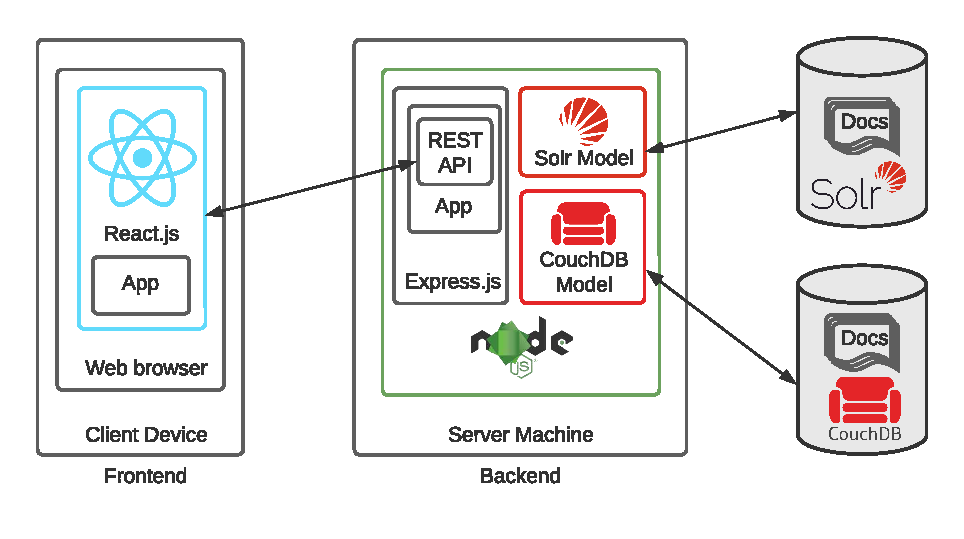
\includegraphics[width=140mm]{../img/architecture}
\caption{Schéma architektury, adaptováno z diagramu MERN aplikace \citep{mern-stack}.}
\label{obr02:architecture}
\end{figure}

Předzpracování dat bude klíčovou fází řešení spolu s~prezentační vrstvou na straně klienta. Serverová část aplikace bude vystupovat pouze jako prostředník mezi klientem a~databází, respektive platformou Solr pro vyhledávací dotazy. Jejím úkolem bude zprostředkování požadovaných dat z~perzistovaného úložiště, která téměř beze změny předá klientovi. Tento přístup si vybere daň v~podobě obsáhlejší databáze, neboť budeme ukládat i~taková data, která bychom dokázali vygenerovat z~ostatních informací. Nejdůležitější instancí tohoto opakování dat bude uložení JSON-LD reprezentace a~zároveň strukturovaných dat v~rámci každého dokumentu receptu. Strukturovaná data by bylo možné při každém dotazu odvodit z JSON-LD nebo naopak. Přesunuli bychom ale komplexitu převodu z~jednorázové fáze předzpracování na samotnou aplikaci, ať už na straně serveru či klienta. Příprava dat pro prezentaci by navíc při každém dotazu trvala o~něco déle, což by se při větším množství dat mohlo negativně odrazit na svižnosti aplikace a~tranzitivně na uživatelském zážitku.

\section{Příprava dat}

V~předchozí kapitole jsme si představili řadu alternativ pro získání datasetů s~recepty a~následně doplňujících informací k~ingrediencím. Dle požadavků aplikace potřebujeme minimálně $50\,000$ receptů z~aspoň $2$ různých zdrojů. Také vyžadujeme integraci $2$ nebo více znalostních grafů s~otevřenými daty. Nemáme spodní limit na počet ingrediencí, které musíme ze znalostních grafů extrahovat. Záleží totiž na úspěšnosti propojení našich ingrediencí s~entitami ze znalostních grafů, která se projeví až při praktickém testu.

Přípravu dat můžeme dále rozdělit na $2$ základní fáze a~to extrakci a čištění dat. Ne všechna data jsou totiž vhodná pro přímou prezentaci uživateli. Jak jsme zmiňovali v~minulé kapitole, volně dostupné datasety s~recepty často cílí spíše na oblast strojového učení. Extrahovaná data je tedy potřeba manuálně zkontrolovat a navrhnout heuristiku, pomocí které bude většina dat normalizována, případně odstraněna při nesplnění zadaných kritérií. Vzhledem k charakteru problému a~omezené časové dotaci nelze na každou datovou sadu aplikovat deterministické řešení, které by eliminovalo všechny anomálie, proto se v~některých případech musíme spokojit s~heuristikou.

\subsection{Extrakce dat}

Na tomto místě je vhodné rozhodnout, které ze zdrojů dat popsaných v~předchozí kapitole nakonec použijeme v~rámci našeho řešení. U~dat k~ingrediencím máme na výběr znalostní grafy DBpedia a~Wikidata, případně méně obsáhlý RDF dataset z~projektu FoodKG. Pro maximalizaci počtu nalezených výsledků se zaměříme na grafy DBpedia a~Wikidata. V~kategorii receptů zvolíme kombinaci statických datových sad s~recepty a~generování vlastních datasetů pomocí procesu web scraping. Během implementace vlastní extrakce dat zapojíme knihovnu Apify pro Node.js a~její koncept tzv.~\emph{actorů}, což jsou programy určené primárně pro cloudovou platformu Apify, kde jsou spouštěny uvnitř Docker kontejnerů. Mohou mít za úkol automatizaci libovolných úkonů prováděných ve webovém prohlížeči, od jednoduchého posílání e-mailů až po extrakci dat z~komplexních webových stránek. Actory lze pomocí nástroje Apify CLI spouštět i~lokálně, čehož pro jednodušší konfiguraci využijeme v~našem řešení. Volitelně lze aktivovat rotování IP adres, které chrání naši vlastní IP adresu před dočasným či dokonce trvalým zablokováním a~zlepšuje poměr úspěšných požadavků. Vzhledem k~obecně nižší míře blokování ze strany aplikací s~recepty by využití proxy nemělo být nutné, je ale vhodné. Počet současně odesílaných požadavků omezíme na rozumnou hranici, abychom zamezili přetížení zpracovávané webové aplikace.

\subsubsection{Food.com}

Vzhledem k~požadavkům definovaným v~předchozí kapitole nám bude vyhovovat dataset Food.com Recipes and~Interactions dostupný na platformě Kaggle, z~něhož jsme schopni získat přibližně $180\,000$ identifikátorů receptů a~také seznam normalizovaných ingrediencí. Dle provedené analýzy není vhodné použít textová data v~prezentační vrstvě vzhledem k jejich lowercase formátu. Navrhneme tedy řešení z~oblasti web scrapingu, které na vstupu přijme URL adresy s~detaily receptů, na každou adresu odešle požadavek GET a~z~HTML odpovědi extrahuje JSON-LD data. Program bude mít možnost získat přes CSS selektory libovolná data z~načteného HTML, pokud by v JSON-LD reprezentaci nebyla obsažena, nebo byla méně strukturována. Programu tedy přidělíme také zodpovědnost za tvorbu strukturovaných dat, která do vygenerovaného datasetu uloží ke každému receptu spolu s~jeho JSON-LD podobou. Strukturovanými daty zde rozumíme čas přípravy, počet porcí, klíčová slova, která jsou v~JSON-LD uložena ve společném řetězci namísto pole řetězců, hodnocení receptu s~počtem recenzí, nutriční hodnoty s~jednotkami měření a~ingredience s~množstvím a~jednotkou oddělenými od ostatního textu.

Extrahované výsledky uložíme do společného JSON souboru, který následně sloučíme s~informacemi z~datasetu Food.com Recipes and~Interactions. Poskytnutý JSON-LD například neobsahuje kompletní informace o~autorovi, ale pouze jeho jméno. Dle samotného jména nejsme schopni autora jednoznačně identifikovat a~zjistit odkaz na jeho profil v~rámci aplikace Food.com. URL adresa autora je totiž sestavena z~jeho unikátního id, které máme k~dispozici právě v~datasetu z~Kaggle. Dále budeme chtít extrahované recepty rozšířit o~normalizované ingredience, abychom nemuseli navrhovat vlastní heuristiku a~usnadnili si pozdější mapování ingrediencí na entity ze znalostních grafů. Po sloučení všech potřebných dat provedeme finální čištění a následně recepty jako JSON dokumenty uložíme do databáze.

Výše popsané řešení extrakce dat z~Food.com má nevýhodu z~pohledu škálovatelnosti. Maximální počet receptů, které jsme schopni získat, je roven počtu receptů v~datasetu z~Kaggle. Celkový počet receptů na stránce Food.com se od doby pořízení datasetu zvětšil více než dvakrát na aktuálních $526\,851$ receptů. Nicméně i~s~naším zjednodušeným programem vyžadujícím připravené URL adresy detailů receptů jsme schopni získat téměř kompletní data. Zmíněný dataset Recipe1M+ v~době psaní této práce obsahuje téměř $510\,000$ URL adres receptů z~aplikace Food.com. Při potřebě většího škálování bychom mohli využít tato URL, neměli bychom k~nim ovšem normalizované ingredience a~byli bychom omezeni striktně akademickým využitím. Pro účely naší práce se spokojíme s~horní hranicí $180\,000$ receptů s~normalizovanými ingrediencemi. Tyto recepty jsou dle autorů datasetu Majumdera a~kol. podmnožinou receptů z~let $2000$-$2018$, které mají aspoň $3$~kroky postupu a~počet ingrediencí v rozmezí $4$ a $20$ \citep{majumder-etal-2019-generating}. Kód souvisejícího projektu pro generování personalizovaných receptů je dostupný jako open-source na platformě GitHub, lze tedy předpokládat, že datovou sadu lze využívat bez omezení.

\subsubsection{Allrecipes}

Jako další zdroj receptů si vybereme webovou aplikaci Allrecipes. Pro ni sice nemáme k~dispozici podrobný dataset jako u~stránky Food.com, vystačíme si ale s~vlastní extrakcí dat prostřednictvím Apify actora. Mohli bychom využít prakticky stejnou šablonu, jako u~programu pro zpracování Food.com. S~využitím datasetu Recipe1M+ dokážeme získat $49\,000$ URL adres detailů receptů. Poměrně snadno bychom ale dokázali navrhnout pokročilejší řešení extrakce dat, které by dynamicky procházelo celou webovou stránku Allrecipes, našlo detaily všech receptů a~z~nich extrahovalo aktuální data. Tímto přístupem bychom odstranili závislost na datové sadě Recipe1M+ a~získali větší počet výsledků. Pro nalezení všech receptů bychom sice museli zpracovat více požadavků, aplikace Allrecipes ale využívá interní API, přes které lze získat URL adresy $48$ receptů v~rámci $1$~požadavku. Celkový počet receptů na Allrecipes se aktuálně pohybuje kolem $50\,000$, což lze zjistit spuštěním vyhledávání bez jakýchkoli nastavených filtrů.

Webová aplikace Allrecipes nabízí svým uživatelům ve vztahu k~ingrediencím vyhledávání dle surovin a~také možnost přizpůsobit množství ingrediencí požadovanému počtu porcí. Tato skutečnost naznačuje, že si aplikace přísady interně spravuje ve strukturované podobě, přestože v~přiloženém JSON-LD je poskytuje jako prostý text včetně množství a jednotky měření. Zaměřme se na konkrétní ingredienci uvnitř HTML dokumentu vybraného receptu. Můžeme si povšimnout, že v~atributech příslušného \texttt{input} elementu jsou uložena strukturovaná data ingredience v~následujícím formátu (ukázka z~receptu \texttt{92462} pro surovinu kuřecí vývar):

\begin{code}
<input
    class="checkbox-list-input"
    data-tracking-label="ingredient clicked"
    data-quantity="½"
    data-init-quantity="0.5"
    data-unit="cup"
    data-ingredient="chicken broth"
    data-unit_family="volumetric"
    data-store_location="Soup"
    type="checkbox"
    value="(14.5 ounce) can chicken broth"
    id="recipe-ingredients-label-92462-0-4">
\end{code}
%$

Z atributů elementu \texttt{input} dokážeme rozpoznat název, množství i~jednotku ingredience. Tyto užitečné informace v~rámci extraktoru zacílíme pomocí CSS selektorů. Díky tomu získáme výrazně přesnější data, než prostřednictvím normalizovaných ingrediencí z~datasetu Food.com Recipes and~Interactions.

\subsubsection{DBpedia}

V~první fázi extrakce dat z~grafu DBpedia potřebujeme identifikovat entity ingrediencí, které dokážeme namapovat na jména surovin z~jednotlivých receptů. K~tomu využijeme nástroj Silk Workbench a~vytvoříme RDF tvrzení s~IRI adresami ingrediencí spojenými vztahem \texttt{owl:sameAs}. V~rámci úlohy linkování navrhneme transformaci textu ingrediencí, která dokáže názvy propojit i~s~mírnými odlišnostmi ve formátu, čísle nebo pádu slov. Pro každou ingredienci vyjádřenou pomocí DBpedia IRI pak extrahujeme vybrané informace včetně názvu, popisu, obrázku, kategorií a~místa původu. Z~nutričních hodnot se zaměříme na energii v~kaloriích nebo kilojoulech, dále na obsah tuku, sacharidů, bílkovin, vlákniny, cholesterolu a~cukru. Aktuálně se zabýváme pouze anglickou lokalizací aplikace, všechna textová data tedy omezíme na anglické výsledky. Jedinou povinnou informací bude název (label) ingredience, všechna ostatní data budou nepovinná, neboť se formát i~množství dat napříč ingrediencemi výrazně liší.

Teoreticky bychom mohli vytvořit jeden společný SPARQL dotaz pro všechny ingredience a~ten odeslat na DBpedia SPARQL endpoint. Dotaz by ale v~závislosti na počtu nalezených spojení mezi surovinami mohl skončit příliš dlouhý a~nenechal by prostor pro škálování. Zvolíme tedy alternativní řešení --- dynamicky vytvoříme sadu dotazů stejného formátu, každý s~přibližně $20$ IRI adresami entit ingrediencí. Tyto dotazy zpracujeme postupně a~výsledky uložíme do společného JSON datasetu s~detaily ingrediencí. Výsledky si navíc od SPARQL endpointu můžeme vyžádat v~řadě různých formátů. Pro naše účely bude nejpraktičtější formát JSON-LD, jehož obsah využijeme v~hlavičkách HTML dokumentů ingrediencí. Se SPARQL endpointem lze komunikovat přes grafické rozhraní ve webovém prohlížeči nebo prostřednictvím HTTP GET požadavků. Pro snadnější automatizaci procesu extrakce využijeme druhou možnost, kde obsah dotazu předáme na místě query parametru s~názvem \texttt{query}.

\subsubsection{Wikidata}

IRI adresy požadovaných entit z~Wikidata získáme opět pomocí aplikace Silk Workbench. Také samotný proces extrakce dat bude probíhat analogicky k~postupu pro data z~DBpedia. I~zde využijeme HTTP GET požadavky na SPARQL endpoint, kde prostřednictvím query parametrů předáme obsah dotazu a~požadovaný formát výsledku. Projekt Wikidata neposkytuje reprezentaci JSON-LD, vystačíme si ale s~běžným JSON formátem, který lze vyžádat přes hodnotu query parametru \texttt{format} nastavenou na \texttt{json}. Z~této reprezentace pak sami vytvoříme odpovídající JSON-LD formát, který je vhodný pro strukturovaná data v~hlavičce HTML dokumentu.

\subsection{Čištění dat}

V~rámci fáze čištění dat potřebujeme extrahovaná data převést do formátu vhodného k~prezentaci koncovému uživateli. Jednotlivé kroky procesu čištění mohou být rozloženy do více míst přípravy dat. Již během extrakce dat probíhá odstranění mezer a~znaků nového řádku na okrajích řetězců. Dále je potřeba se vypořádat se znaky, které jsou kvůli vnoření v~HTML dokumentu kódovány jinými znaky, aby bylo zajištěno jejich korektní zobrazení. Takové znaky se vyskytují např. v~extrahovaných JSON-LD dokumentech, před jejich uložením do databáze tedy provedeme dekódování. Rekurzivně projdeme obsah každého objektu načteného z~JSON-LD dokumentu a~všechny řetězce dekódujeme s~využitím open-source knihoven pro Node.js. V~našem řešení integrujeme knihovny \texttt{html-escaper} a~\texttt{html-entities} dostupné přes správce balíčků npm.

Dále jsme se rozhodli z~vyhledávání vyřadit recepty bez fotografie, které lze identifikovat a~přeskočit již během fáze extrakce nebo následně při ukládání do databáze, případně až při tvorbě dokumentů pro vyhledávací platformu Solr. Zvolíme poslední způsob, recepty tedy uložíme do vlastní databáze bez ohledu na přítomnost jejich obrázků. Díky tomu budeme mít v~budoucnu snadnou cestu k~využití zbývajících receptů bez fotografií, ať už pro účely strojového učení nebo i~zobrazení uživateli, pokud by větší nabídka receptů výrazně převážila nevýhodu absence ilustračních fotografií.

Také data k~ingrediencím budou vyžadovat významné čištění. V~datasetu Food.com Recipes and~Interactions máme k~dispozici přibližně $8\,000$ unikátních ingrediencí. Co nejvíce z~nich bychom chtěli nabídnout uživateli v~rámci našeptávače ve vyhledávání dle ingrediencí. Pro tento účel názvy ingrediencí převedeme do estetičtějšího formátu s~velkým počátečním písmenem. Po manuální kontrole seznamu ingrediencí ale narazíme na řadu slov, která se mezi suroviny dostala omylem vlivem chybného parsování jmen ingrediencí. Nebudeme zde uvádět kompletní výčet, typicky se ale jedná o~názvy jednotek měření nebo obecné fragmenty ingrediencí, které samy o~sobě žádnou ingredienci nepředstavují (např. samostatná slova \texttt{clove}, \texttt{seed}, \texttt{extract}, která by byla validní pouze v~kontextu typu \texttt{garlic clove}, \texttt{sesame seed} a~\texttt{vanilla extract}). Vzhledem k~velkému počtu ingrediencí navrhneme heuristiku čištění pomocí regulárních výrazů. Zaměříme se zejména na nejčastěji používané ingredience, které budou zobrazeny v~horní části našeptávače. Pro potřeby našeptávače nastavíme limit maximálního počtu slov ingredience a~to na hodnotu $3$. Pro mapování na entity ze znalostních grafů ale využijeme původní sadu ingrediencí bez omezení počtu slov.

S~normalizovanými ingrediencemi z~Food.com Recipes and~Interactions souvisí další problém --- nejsou přiřazeny ke všem receptům z~datasetu. Texty surovin sice využijeme z~extrahovaného JSON-LD, normalizované ingredience ale potřebujeme k~propojení s~informacemi z~grafů DBpedia a~Wikidata. Recepty bez normalizovaných ingrediencí tedy musíme projít a~pro každou jejich přísadu zkusit na základě prostého textu nalézt co nejbližší shodu s~některou z~normalizovaných ingrediencí. Pro zjednodušení budeme akceptovat pouze přesné shody, přestože nám tímto způsobem může část ingrediencí uniknout, neboť mohou být v~prostém textu uvedeny v~jiném pádě nebo čísle.

Dalším úkolem čisticí fáze bude normalizace JSON-LD reprezentace ingrediencí z~grafu DBpedia. Ve srovnání s~projektem Wikidata jsme zde ve výhodě, jelikož data obdržíme přímo v JSON-LD. Zároveň ale extrahujeme data pro více ingrediencí najednou a~každá z~nich má vlastní schéma, které se většinou plně neshoduje s~ostatními entitami. Při skupinové extrakci dat se ale musí vytvořit univerzální schéma, kterým lze vyjádřit všechny obsažené informace. Naším úkolem bude projít uložené kolekce ingrediencí a~pro každou ingredienci vytvořit minimální JSON-LD kontext, kterým ji lze popsat. Jednotlivé ingredience pak do databáze uložíme vždy s~vlastním JSON-LD kontextem. V~praxi se totiž často stává, že objevíme pod stejnou vlastností různé typy hodnot. Např. region původu ingredience může nést IRI příslušné entity z~grafu DBpedia, ale také prostý literál. Skutečný typ musí být řádně definován kontextem JSON-LD dokumentu. Proto není vhodné mít společný kontext pro všechny ingredience, neboť by u~některých vlastností existoval duplicitní popis použitých typů.

\section{Databázový model}

Pro uložení dat receptů a~ingrediencí zvolíme dokumentovou databázi Apache CouchDB, často označovanou zkráceně CouchDB. Nejbližší alternativou z~řad NoSQL dokumentových databází by byl systém MongoDB, který je stejně jako databáze CouchDB open-source. Pro naše potřeby by dobře fungoval libovolný z~těchto systémů, neboť chceme využít zejména konceptu dokumentových databází, které typicky nevyžadují striktní schéma a~umožňují tak kompaktní uložení různorodých dat ve formátu JSON. To je v~naší doméně cenná vlastnost, neboť plánujeme ukládat data poměrně komplexní struktury --- vezměme v~potaz například JSON-LD formát s~mnoha zanořenými objekty. Také extrahujeme data z~více zdrojů a~vyžadování zcela jednotného rozhraní by nám v~některých situacích zbytečně zkomplikovalo práci. Na základě jakého kritéria tedy rozhodujeme mezi variantami CouchDB a~MongoDB?

Databázi budeme pokládat pouze velmi jednoduché dotazy, totiž vyžádání dokumentu na základě jeho unikátního id. Pro práci s~databází preferujeme použití Node.js knihovny, což je splnitelné oběma databázovými systémy CouchDB i~MongoDB, neboť oba poskytují oficiální ovladač pro Node.js. K~obsluze složitějších vyhledávacích dotazů využijeme systém Apache Solr, který si bude držet vlastní podmnožinu dat z~dokumentů uložených v~databázi. Kombinací Apache CouchDB s~Apache Solr bychom sjednotili technologie z~dílny Apache Software Foundation. Zároveň by se nám v~budoucnu mohla hodit podpora současného čtení a~zápisu, kterou systém CouchDB nabízí \citep{mongodb-vs-couchdb}. Co se týče dat s~recepty či ingrediencemi, není potřeba vyžadovat, aby se uživateli vždy zobrazila verze se všemi aktualizacemi. Např. vybraný recept zůstává relevantní i~v~momentě, kdy zrovna současný nebo jiný uživatel přidává k~receptu nové hodnocení. Díky systému verzování dokumentů, který CouchDB implementuje, se nemusíme obávat o~dostupnost dat během jejich aktualizace.

V~systému CouchDB lze snadno vytvářet a~spravovat více databází neboli kolekcí dokumentů. Vytvoříme tedy samostatné databáze pro recepty a~ingredience, přičemž oba typy dokumentů v~sobě budou mít uložena strukturovaná data i~JSON-LD reprezentaci. Na rozdíl od tradičních relačních databází nemusíme předem definovat žádná schémata ukládaných dat.

S~CouchDB můžeme komunikovat přes webové rozhraní skrze přehlednou aplikaci Fauxton, pomocí REST~API nebo prostřednictvím již zmíněné knihovny v~prostředí Node.js. Pro automatizované nahrávání dokumentů využijeme oficiální knihovnu \texttt{nano}. S~velikostí našeho projektu si můžeme dovolit při nahrávání nových dat nejprve stávající data odstranit a~poté je vložit do čisté databáze. Kdybychom totiž chtěli dokumenty aktualizovat, potřebovali bychom u~každého z~nich poskytnout aktuální verzi, což by pro přepsání celé databáze byl zbytečně komplikovaný postup. S~rostoucím počtem dokumentů bychom ale nejspíše museli přistoupit na aktualizaci dat namísto jejich odstraňování a~opětovného nahrávání, neboť již pro přidání kolekce o~velikosti $50\,000$ dokumentů se pohybujeme v~řádu delších minut.

\section{Indexy}

Pro uložení dokumentů do databáze CouchDB není potřeba specifikovat žádné schéma. Během konfigurace platformy Apache Solr pro vyhledávání se ovšem bez striktně definovaného schématu neobejdeme. Respektive abychom byli přesní, Solr dokáže na základě vložených dat odvodit schéma dynamicky, často ale nezvolí datový typ správně a~navíc je při výběru zbytečně generický. Představme si libovolný řetězec z~dokumentu receptu, například text jedné ingredience. Pokud Solr nenajde ve schématu žádnou definici typu u~vlastnosti ingredience, vytvoří pro ni dynamický index typu \texttt{string}. Na první pohled se zdá být vše v~pořádku, když si ale projdeme dostupné typy, najdeme mezi nimi i~podstatně specifičtější variantu \texttt{text\_en}. Typ anglického textu je pro naši aktuální lokalizaci ideální, neboť nabízí vestavěnou podporu skloňování a~časování anglických slov. V~praxi nám pomůže najít více relevantních výsledků. Uživatel může zadat například ingredienci \texttt{tomatoes}, Solr provede normalizaci vyhledávaného termínu a~vrátí recepty obsahující mezi surovinami nejen slova \texttt{tomatoes}, ale také \texttt{tomato}.

Prvním krokem pro práci s~platformou Solr je tedy kompletní návrh schématu pro dokumenty receptů. Pro vytvoření schématu využijeme skript operující nad REST~API poskytovaným systémem Solr, čímž proces automatizujeme a~usnadníme případnou migraci na jiné zařízení. Solr umožňuje data rozdělit do tzv.~jader, založíme tedy samostatné jádro pro dokumenty s~recepty a~vytvoříme infrastrukturu, která umožní snadné přidání nového jádra, pokud by v~budoucnu bylo potřeba. V~rámci současných požadavků aplikace by se mohlo zdát, že budeme vyhledávací schopnosti platformy Solr potřebovat i~pro dokumenty ingrediencí, konkrétně pro řešení našeptávače surovin. Seznam doporučených přísad by se totiž měl aktualizovat na základě vstupu uživatele. Po napsání každého nového znaku se musí zobrazit pouze ingredience, které odpovídají vyhledávanému výrazu. Přirozeně nebereme v~potaz velikost písmen a~vzhledem k~výhradně anglické lokalizaci se v~současnosti nezabýváme ani diakritikou. Využití systému Solr by nám pomohlo nabídnout více relevantních ingrediencí, neboť bychom vyhledávaný výraz mohli interpretovat jako anglický text a~poradit si tak s~jeho formátem v~různých tvarech a časech. Kvůli každému napsanému znaku bychom ale museli odeslat dotaz serveru hostícímu instanci Solr, což by generovalo poměrně významné zpoždění vlivem komunikace po síti. Spokojíme se tedy s~jednodušší architekturou našeptávače --- vyžádáme si všechny ingredience najednou a~zobrazení relevantních návrhů během psaní vyřešíme na straně klienta. Jak lze ale získat seznam všech unikátních ingrediencí, pokud máme v~Solr uloženy pouze dokumenty receptů? Odpovědí je fasetové vyhledávání.

\subsection{Fasetové vyhledávání}

Fasetové vyhledávání, označované také jako fasetová navigace, je způsob interakce, během které uživatel filtruje výsledky výběrem validních hodnot fasetového klasifikačního systému. Tento styl vyhledávání nevyžaduje hierarchické uspořádání nabízených možností, díky čemuž lze filtry přidávat i~odebírat v~libovolném pořadí. Navíc uživatel typicky předem zná počet výsledků, které se po aplikování daného filtru zobrazí \citep{faceted-search}. V~kontextu naší aplikace se fasetová navigace hodí pro jednotlivé vlastnosti vyhledávání, jakými jsou nejen ingredience, ale také klíčová slova, kategorie, typ kuchyně, čas přípravy či hodnocení. Každý z~těchto filtrů je zcela nezávislý, není tedy žádoucí vytvářet kolem nich hierarchii. Nedávalo by smysl zpřístupnit například vyhledávání dle ingrediencí až po výběru kategorie receptu. Na druhou stranu, výběr kategorií může ovlivnit (respektive omezit) nabídku ingrediencí ve fasetové navigaci a~stejně tak volba určitých ingrediencí může vyřadit některé kategorie receptů.

Platforma Solr poskytuje přímou podporu fasetové navigace nad libovolnými položkami dokumentů. Můžeme tedy například snadno specifikovat fasetové vyhledávání nad ingrediencemi, čímž získáme list unikátních jmen surovin, které se v~celé kolekci receptů vyskytují. Je zde ovšem jisté omezení. Pokud fasetové vyhledávání spustíme přímo nad ingrediencemi, které máme uloženy pod typem anglického textu, Solr nám vrátí pouze transformovaná jména ingrediencí, tak jak je má uložena pro své interní vyhledávání. Data tohoto formátu nejsou vhodná pro prezentaci uživateli, tudíž budeme potřebovat ke každému receptu přiřadit nový seznam ingrediencí určený výhradně pro fasetové vyhledávání. Na úrovni schématu definujeme typ fasetových ingrediencí jako prostý řetězec, nad kterým se neprovedou žádné transformace. Zároveň nastavíme ve schématu tzv. \emph{copy field} z~položky zdrojových ingrediencí do položky fasetových ingrediencí. Díky tomu bude stačit během přidávání dokumentů vložit ingredience pouze do základní položky, přičemž do položky pro fasetové vyhledávání se zkopírují automaticky dle schématu.

\subsection{Zvýraznění nalezených výrazů}

Dalším konceptem, se kterým se během vyhledávání pomocí Solr setkáme, bude tzv. \emph{highlighting} neboli zvýraznění vyhledaných výrazů. Využijeme jej při prezentaci surovin jakožto primárního filtru. U~libovolného receptu na vyhledávací obrazovce bude možné zobrazit kompletní seznam ingrediencí. Pro lepší přehlednost zvýrazníme aktuálně vyhledávané ingredience tučným písmem a~pro přesnou identifikaci těchto pojmů využijeme vestavěnou funkci od platformy Solr. Informace o~zvýrazněných ingrediencích doručíme na frontend aplikace spolu s~dokumenty receptů.

\subsection{Model receptu}

Schéma receptu navrhneme dle požadavků na vlastnosti, podle kterých potřebujeme recepty vyhledávat. Zároveň zde ale patří definice všech položek, které budeme na vyhledávací stránce zobrazovat. Teoreticky bychom mohli platformu Solr využít pouze na vyhledání identifikátorů receptů na základě zadaných indexů a~ostatní informace získat z~databáze CouchDB. Tento přístup by optimalizoval množství paměti využívané systémem Solr a~odstranil poměrně výraznou duplicitu dat. Na druhou stranu by do zpracování vyhledávacích dotazů zanesl větší komplexitu a~časovou prodlevu, která by vznikla nadbytečnou komunikací s~\,CouchDB. Pokud si budeme všechny potřebné informace pro vyhledávací stránku držet v~systému Solr, bude nám stačit zpracovat pouze jeden vyhledávací dotaz pro zobrazení jedné stránky receptů. Rychlé vyhledávání je klíčovou funkcionalitou naší aplikace, proto zde upřednostníme optimalizaci časové složitosti namísto paměťové.

Schéma dokumentu receptu uloženého v~Solr bude následující (jedná se pouze o~ilustrační schéma, kde typy odpovídají standardním typům dle specifikace Solr, nikoli běžně dostupným typům formátu JSON):

\begin{code}
{
    name: text_en,
    description: text_en,
    recipeCategory: text_en,
    ingredients: text_en,
    tags: text_en,
    rating: pfloat,
    reviewsCount: pint,
    stepsCount: pint,
    cookMinutes: pint,
    prepMinutes: pint,
    totalMinutes: pint,
    image: string,
    date: string,
    calories: pint,
    fat: pfloat,
    saturatedFat: pfloat,
    cholesterol: pfloat,
    sodium: pfloat,
    carbohydrate: pfloat,
    fiber: pfloat,
    sugar: pfloat,
    protein: pfloat,
}
\end{code}
%$

Ne všechny obsažené položky nutně využijeme v~první verzi naší prezentační vrstvy (například datum a~počet minut samotné přípravy či vaření pokrmu). Jejich zahrnutím ale usnadníme přidávání nových funkcí typu třídění výsledků na základě data publikace nebo vyřazení receptů, u kterých nestačí pouhá příprava ze syrových ingrediencí a~je potřeba počítat s~vařením. Větší výběr informací nám také umožní jednoduchou iteraci nad různými rozloženími uživatelských obrazovek, což je užitečné při hledání vhodného designu.

\section{Backend}

Jak bylo zmíněno v~úvodní části této kapitoly, serverová část aplikace bude sloužit jako poměrně jednoduchá mezivrstva pro zprostředkování komunikace mezi klientem, platformou Solr a~databází CouchDB. Základy architektury položíme na zvoleném frameworku Express.js pro Node.js, který umožňuje snadnou definici REST API a~delegování přijímaných požadavků na vlastní komponenty. Budeme podporovat $4$~endpointy pro HTTP GET požadavky, jmenovitě získání všech receptů nebo ingrediencí a~vyžádání $1$~receptu či ingredience dle jejich unikátního id. V těle odpovědi na libovolný dotaz budou figurovat data v~JSON formátu, naše rozhraní tedy můžeme označit jako JSON~API. Zároveň budeme pracovat s~query parametry, prostřednictvím kterých předáme serveru informaci o~požadovaných filtrech, počtu výsledků na $1$~stránku a~offsetu pro zajištění funkcionality stránkování.

V~závislosti na zvoleném endpointu se s~dotazem obrátíme na Solr nebo \,CouchDB. Pro oba systémy vytvoříme odpovídající modely spravovaných dokumentů. U~Solr nám bude stačit model pro recepty z~důvodů popsaných v~předchozí sekci. U~CouchDB pak definujeme modely pro recepty i~suroviny. Model bude mít za úkol vytvořit a~uchovat spojení s~úložištěm, přičemž vytvoření instance spojení zajistí příslušná komponenta factory s~využitím návrhového vzoru singleton. Díky němu se vyhneme opětovné inicializaci spojení. Dále bude model schopen vytvořit dotazy na základě informací z~query parametrů a~prostřednictvím navázaného spojení tyto dotazy vyhodnotit nad dokumenty v~Solr nebo CouchDB. Následně přijatá data převede do formátu očekávaného na frontendu aplikace (typicky zjednoduší výchozí schéma odpovědi a~relevantní data uloží s~menší mírou zanoření). Data budou poté ve formátu JSON a~s~příslušným stavovým kódem odeslána klientovi. 

\subsection{JSON API}

Zde soustředíme konkrétní podobu API pro získání JSON dokumentů s~recepty a~ingrediencemi. Prefixem potřebným pro složení kompletní URL adresy je název domény, v~našem vývojovém prostředí \texttt{localhost:5000}.

\subsubsection{Získání všech dokumentů}

Dotaz na recepty využijeme v~kontextu vyhledávací obrazovky. Požadavek obohatíme o~query parametry nesoucí informace o~požadovaných ingrediencích, klíčových slovech, kategoriích a~dalších filtrech. Za normálních okolností si vyžádáme pouze omezené množství výsledků odpovídající počtu receptů na $1$~stránce. Tím získáme odpověď v~podstatně kratším čase, což se projeví dřívějším zahájením renderování výsledků vyhledávání. Chceme uživateli API umožnit nastavení vlastního limitu počtu výsledků, neboť se limit může na frontendu měnit nezávisle na zbytku aplikace. Navíc tím také usnadníme práci vývojářům, kteří by potřebovali z~naší aplikace extrahovat strukturovaná data, neboť by jim stačil výrazně menší počet požadavků. Nastavíme ovšem maximální limit na počet výsledků v~rámci $1$~požadavku, abychom zamezili situacím, kdy se uživatel API pokusí najednou získat všechna data z~naší aplikace.

Ingredience máme uloženy pouze v~databázi CouchDB, dotaz z~endpointu ingrediencí tedy bude směřovat právě tam. S~aktuálními požadavky aplikace si bez tohoto endpointu vystačíme, je ale pravděpodobné, že budeme v~blízké době implementovat encyklopedii všech ingrediencí po vzoru webové aplikace Food.com.

\begin{code}
/api/recipes
/api/ingredients
\end{code}
%$

\subsubsection{Získání dokumentu dle id}

Požadavky směřující na následují endpointy jsou vyřizovány nalezením detailu receptu nebo ingredience v~databázi CouchDB:

\begin{code}
/api/recipes/:recipeId
/api/ingredients/:ingredientId
\end{code}
%$

\section{Frontend}

Návrh klientské vrstvy bude silně ovlivněn charakterem knihovny React, která je založena na designu tzv. \emph{komponent}. Ty mohou být modelovány objektově orientovaným způsobem jako třídy nebo funkcionálním jako samostatné exportované funkce. Autoři dokumentace knihovny React doporučují v~nových projektech využívat primárně funkcionální komponenty a~pro práci se stavem a~životním cyklem komponenty využít tzv. \emph{Hooks}. Většina z~důležitých funkcí, které byly dříve implementovány pouze v~objektových komponentách, je již dostupná funkcionálním komponentám skrze Hooks a~podpora zbývajících funkcí je plánována \citep{class-or-functional}. Architekturu tedy založíme na doporučených funkcionálních komponentách.

\subsection{Funkcionální komponenta}

Jedná se o~jednoduchou funkci přijímající tzv.~\emph{props} na místě parametrů a~s~návratovým typem základního elementu knihovny React. Tyto elementy mohou být zapsány pomocí \emph{JSX}, což je syntaktické rozšíření jazyka JavaScript. Připomíná šablonovací jazyk, neboť kombinuje syntaxi jazyka HTML s~kódem psaným v~JavaScriptu. React zajišťuje renderování JSX elementů do HTML dokumentu prostřednictvím rozhraní DOM \citep{jsx-intro}. Příklad jednoduchého JSX elementu, který se v~HTML vygeneruje jako tag \texttt{h1} s~textem \texttt{Headline}:

\begin{code}
const element = <h1>Headline</h1>;
\end{code}
%$

Ekvivalentem pro vývoj v~jazyce TypeScript je formát \emph{TSX}, který budeme používat v~naší aplikaci. Rozlišujeme čistě prezentační komponenty, které pouze renderují data přijatá přes parametr \texttt{props}, a~stavové komponenty způsobující vedlejší efekty v~podobě změny stavu aplikace.

\subsection{Obrazovky uživatelského rozhraní}

Přestože vyvíjíme single-page aplikaci, počítáme s~více obrazovkami pro pohodlnější navigaci. S~využitím knihovny React Router dokážeme simulovat existenci libovolného množství obrazovek a~zároveň zůstat na jedné stránce bez potřeby opětovného načítání. Tím se odlišíme od tradičních statických aplikací, kterým při každé změně URL včetně query parametrů musí server v~odpovědi poslat odpovídající HTML obsah. Náš přístup má ovšem nevýhodu z~pohledu strojového zpracování, neboť pro vygenerování obsahu stránky potřebujeme v~prohlížeči spustit JavaScript kód. Tím znemožníme zpracování naší aplikace prostřednictvím pouhých HTTP požadavků, což je podstatně jednodušší a~ekonomičtější varianta ve srovnání s~automatizací celého webového prohlížeče. Tento nedostatek ale kompenzujeme transparentním REST API, přes které si lze vyžádat strukturovaná data pomocí HTTP požadavků. Zároveň usnadníme strojové zpracování vyhledávačům, které automatizaci prohlížeče využívají, neboť v~detailech receptů a~ingrediencí zahrneme jejich JSON-LD reprezentaci.

Aplikaci složíme ze $3$ základních uživatelských obrazovek: vyhledávání receptů, detail receptu a~detail ingredience. Všechny obrazovky musí být responzivní a~poradit si s~proměnlivou velikostí obrazovky.

\subsubsection{Vyhledávání receptů}

Domovskou stránku bude tvořit vyhledávání receptů na základě různých kritérií. Primárně bude k~dispozici výběr požadovaných ingrediencí, sekundárně filtry klíčových slov, kategorií, času přípravy, hodnocení a~nutričních hodnot. Všechny filtry bude možné odstranit samostatně i~najednou pomocí společného tlačítka pro smazání. Pro získání přesnějších výsledků bude při vyplňování filtrů k~dispozici našeptávač, který zobrazí známé možnosti a~spolu s~nimi počty receptů, které jsou při výběru tohoto nastavení k~dispozici. Výsledky budou zobrazovány na stránkách s~$24$ nebo $30$ kartami receptů. Přepínání stránek bude umístěno standardně ve spodní části stránky a~zároveň bude aktuální stránka figurovat v~query parametrech pro přímočarou podporu navigace v~historii prohlížeče. Karta receptu bude obsahovat název, popis, obrázek, hodnocení, počet recenzí, čas přípravy a~počet instrukcí. Navíc bude možné rozbalit seznam ingrediencí, ve kterém budou zvýrazněny aktuálně vyhledávané ingredience. Uživatel bude přesměrován na obrazovku s~detailem receptu při stisknutí tlačítka \texttt{View} nebo při kliknutí na obrázek receptu. Konkrétní rozložení obrazovek viz obrázek \ref{obr02:desktop-search-view} pro desktopová zařízení a \ref{obr02:mobile-search-view} pro mobilní zařízení.

\begin{figure}[p]\centering
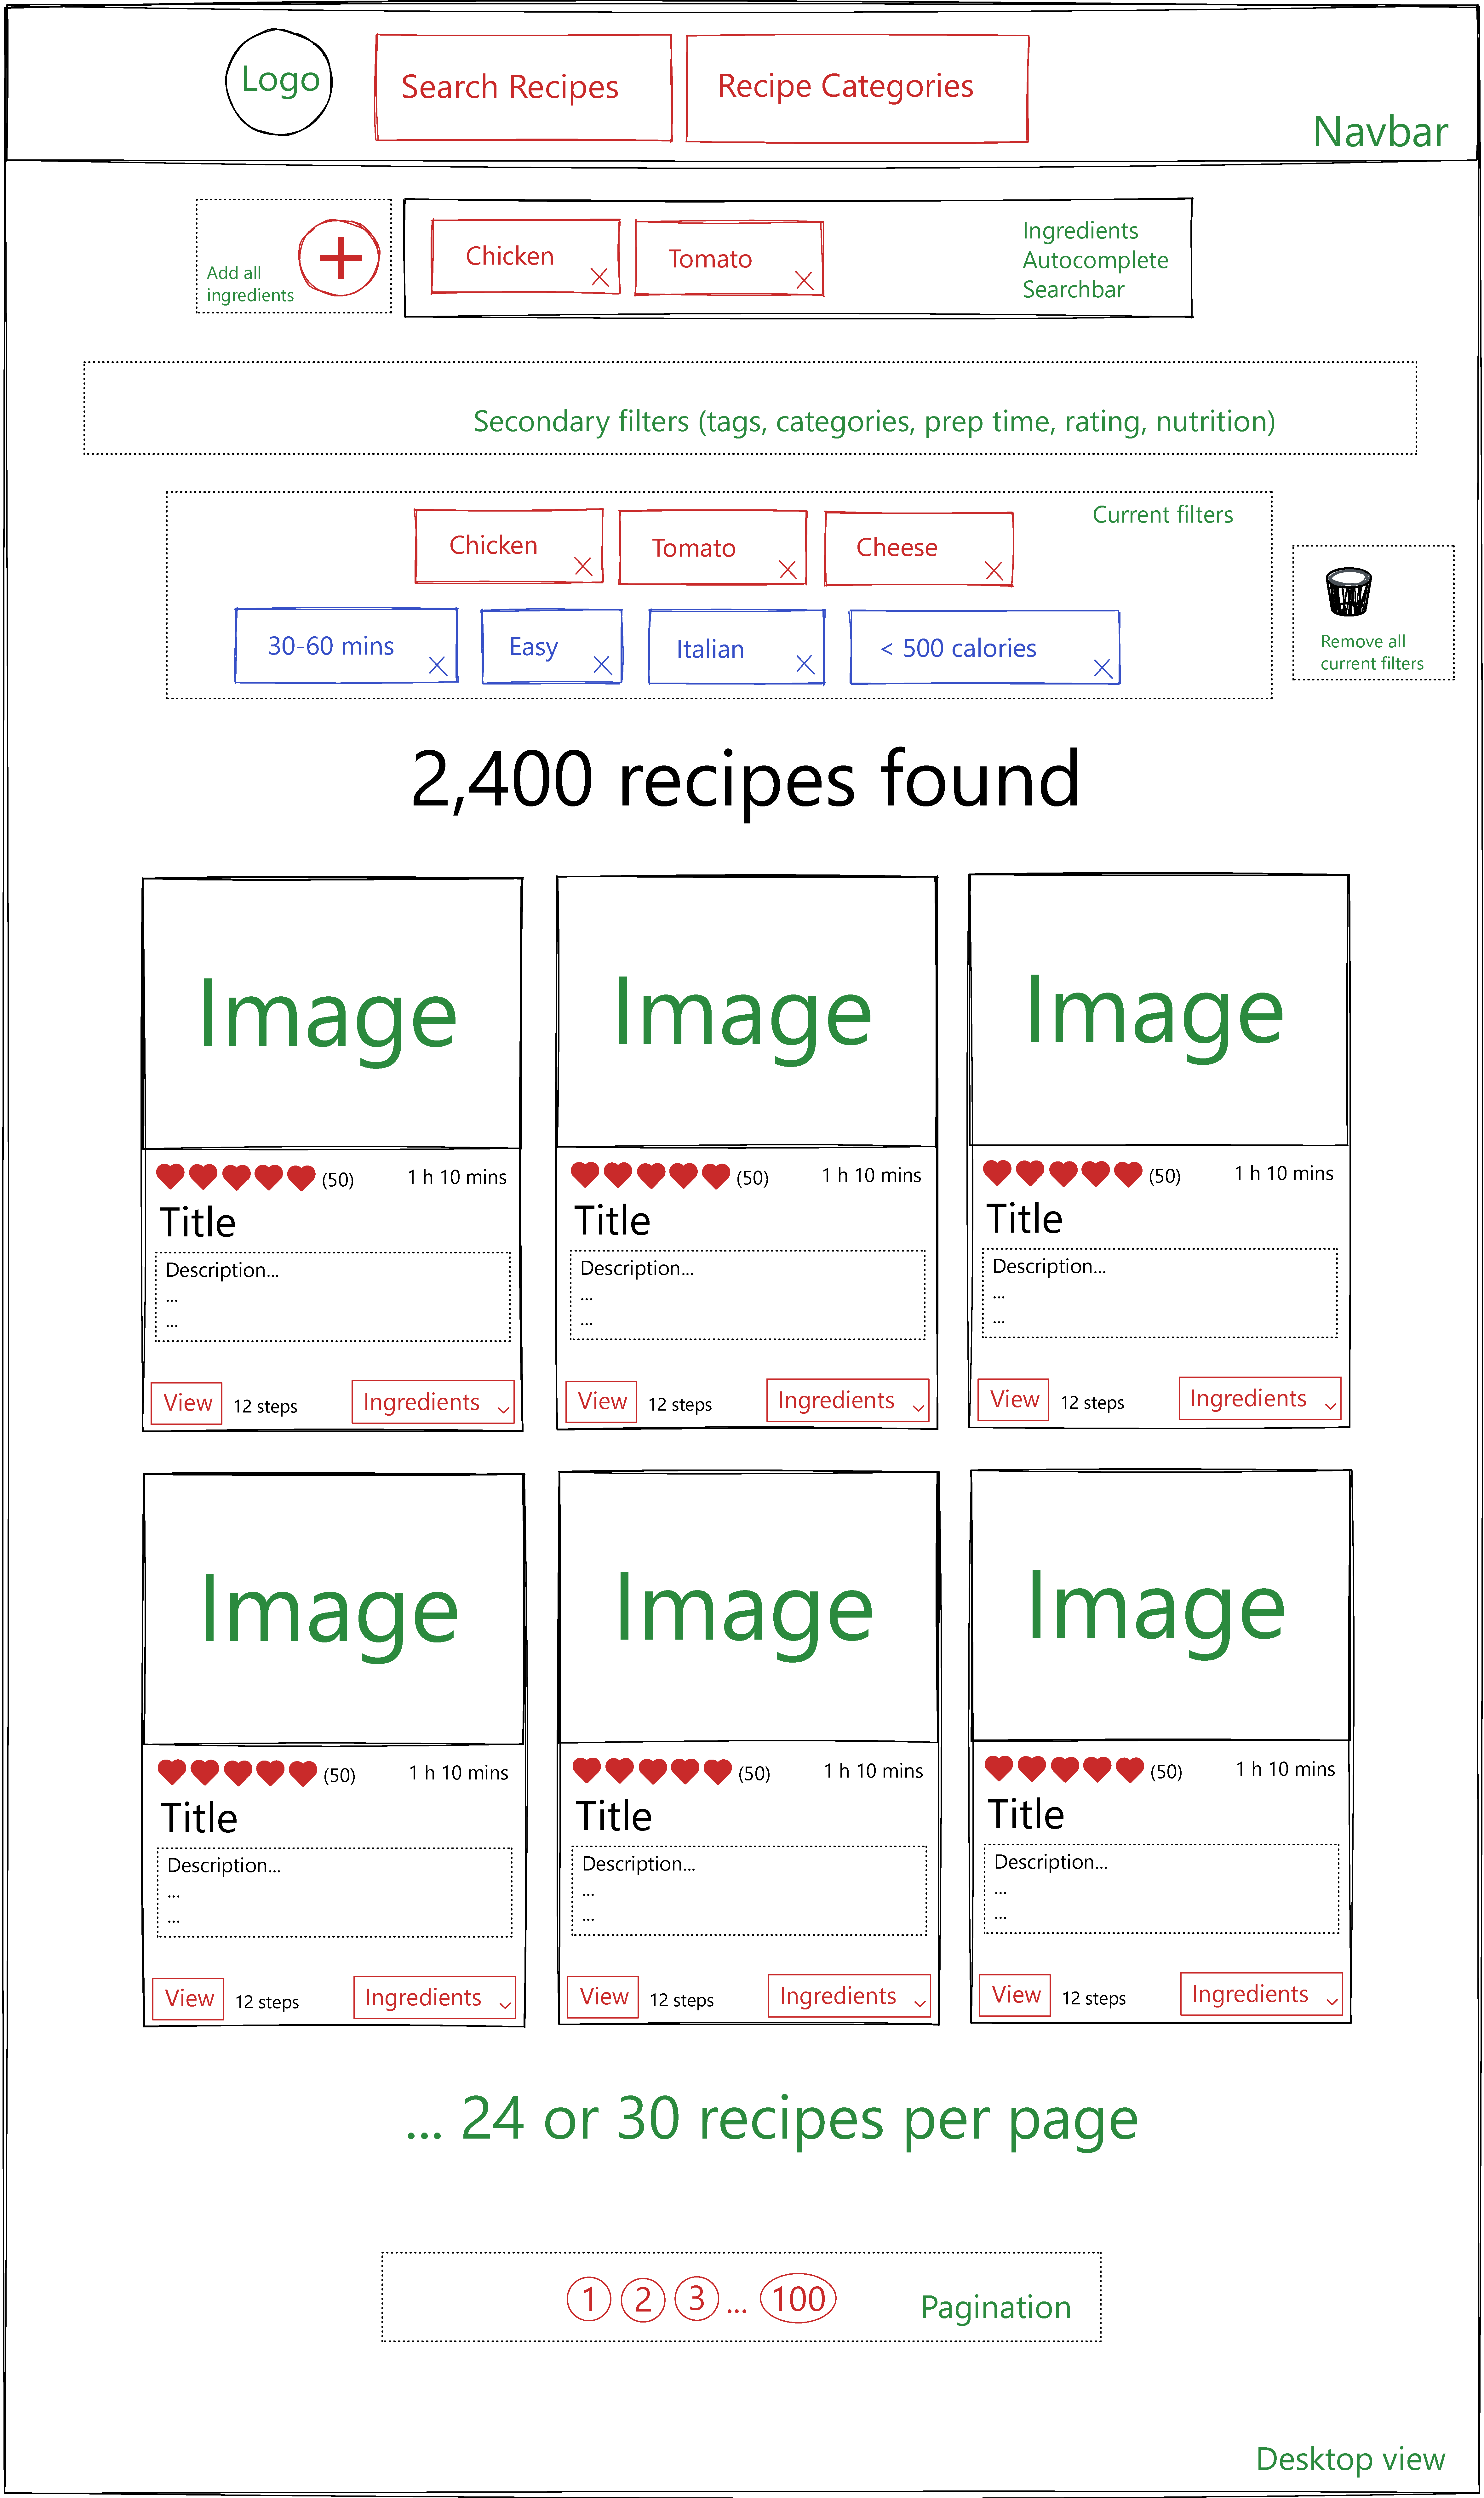
\includegraphics[width=140mm]{../img/desktop-search-view}
\caption{Obrazovka vyhledávání receptů pro desktopová zařízení.}
\label{obr02:desktop-search-view}
\end{figure}

\begin{figure}[p]\centering

\includegraphics[height=230mm]{../img/mobile-search-view}
\caption{Obrazovka vyhledávání receptů pro mobilní zařízení.}
\label{obr02:mobile-search-view}
\end{figure}

\begin{figure}[p]\centering
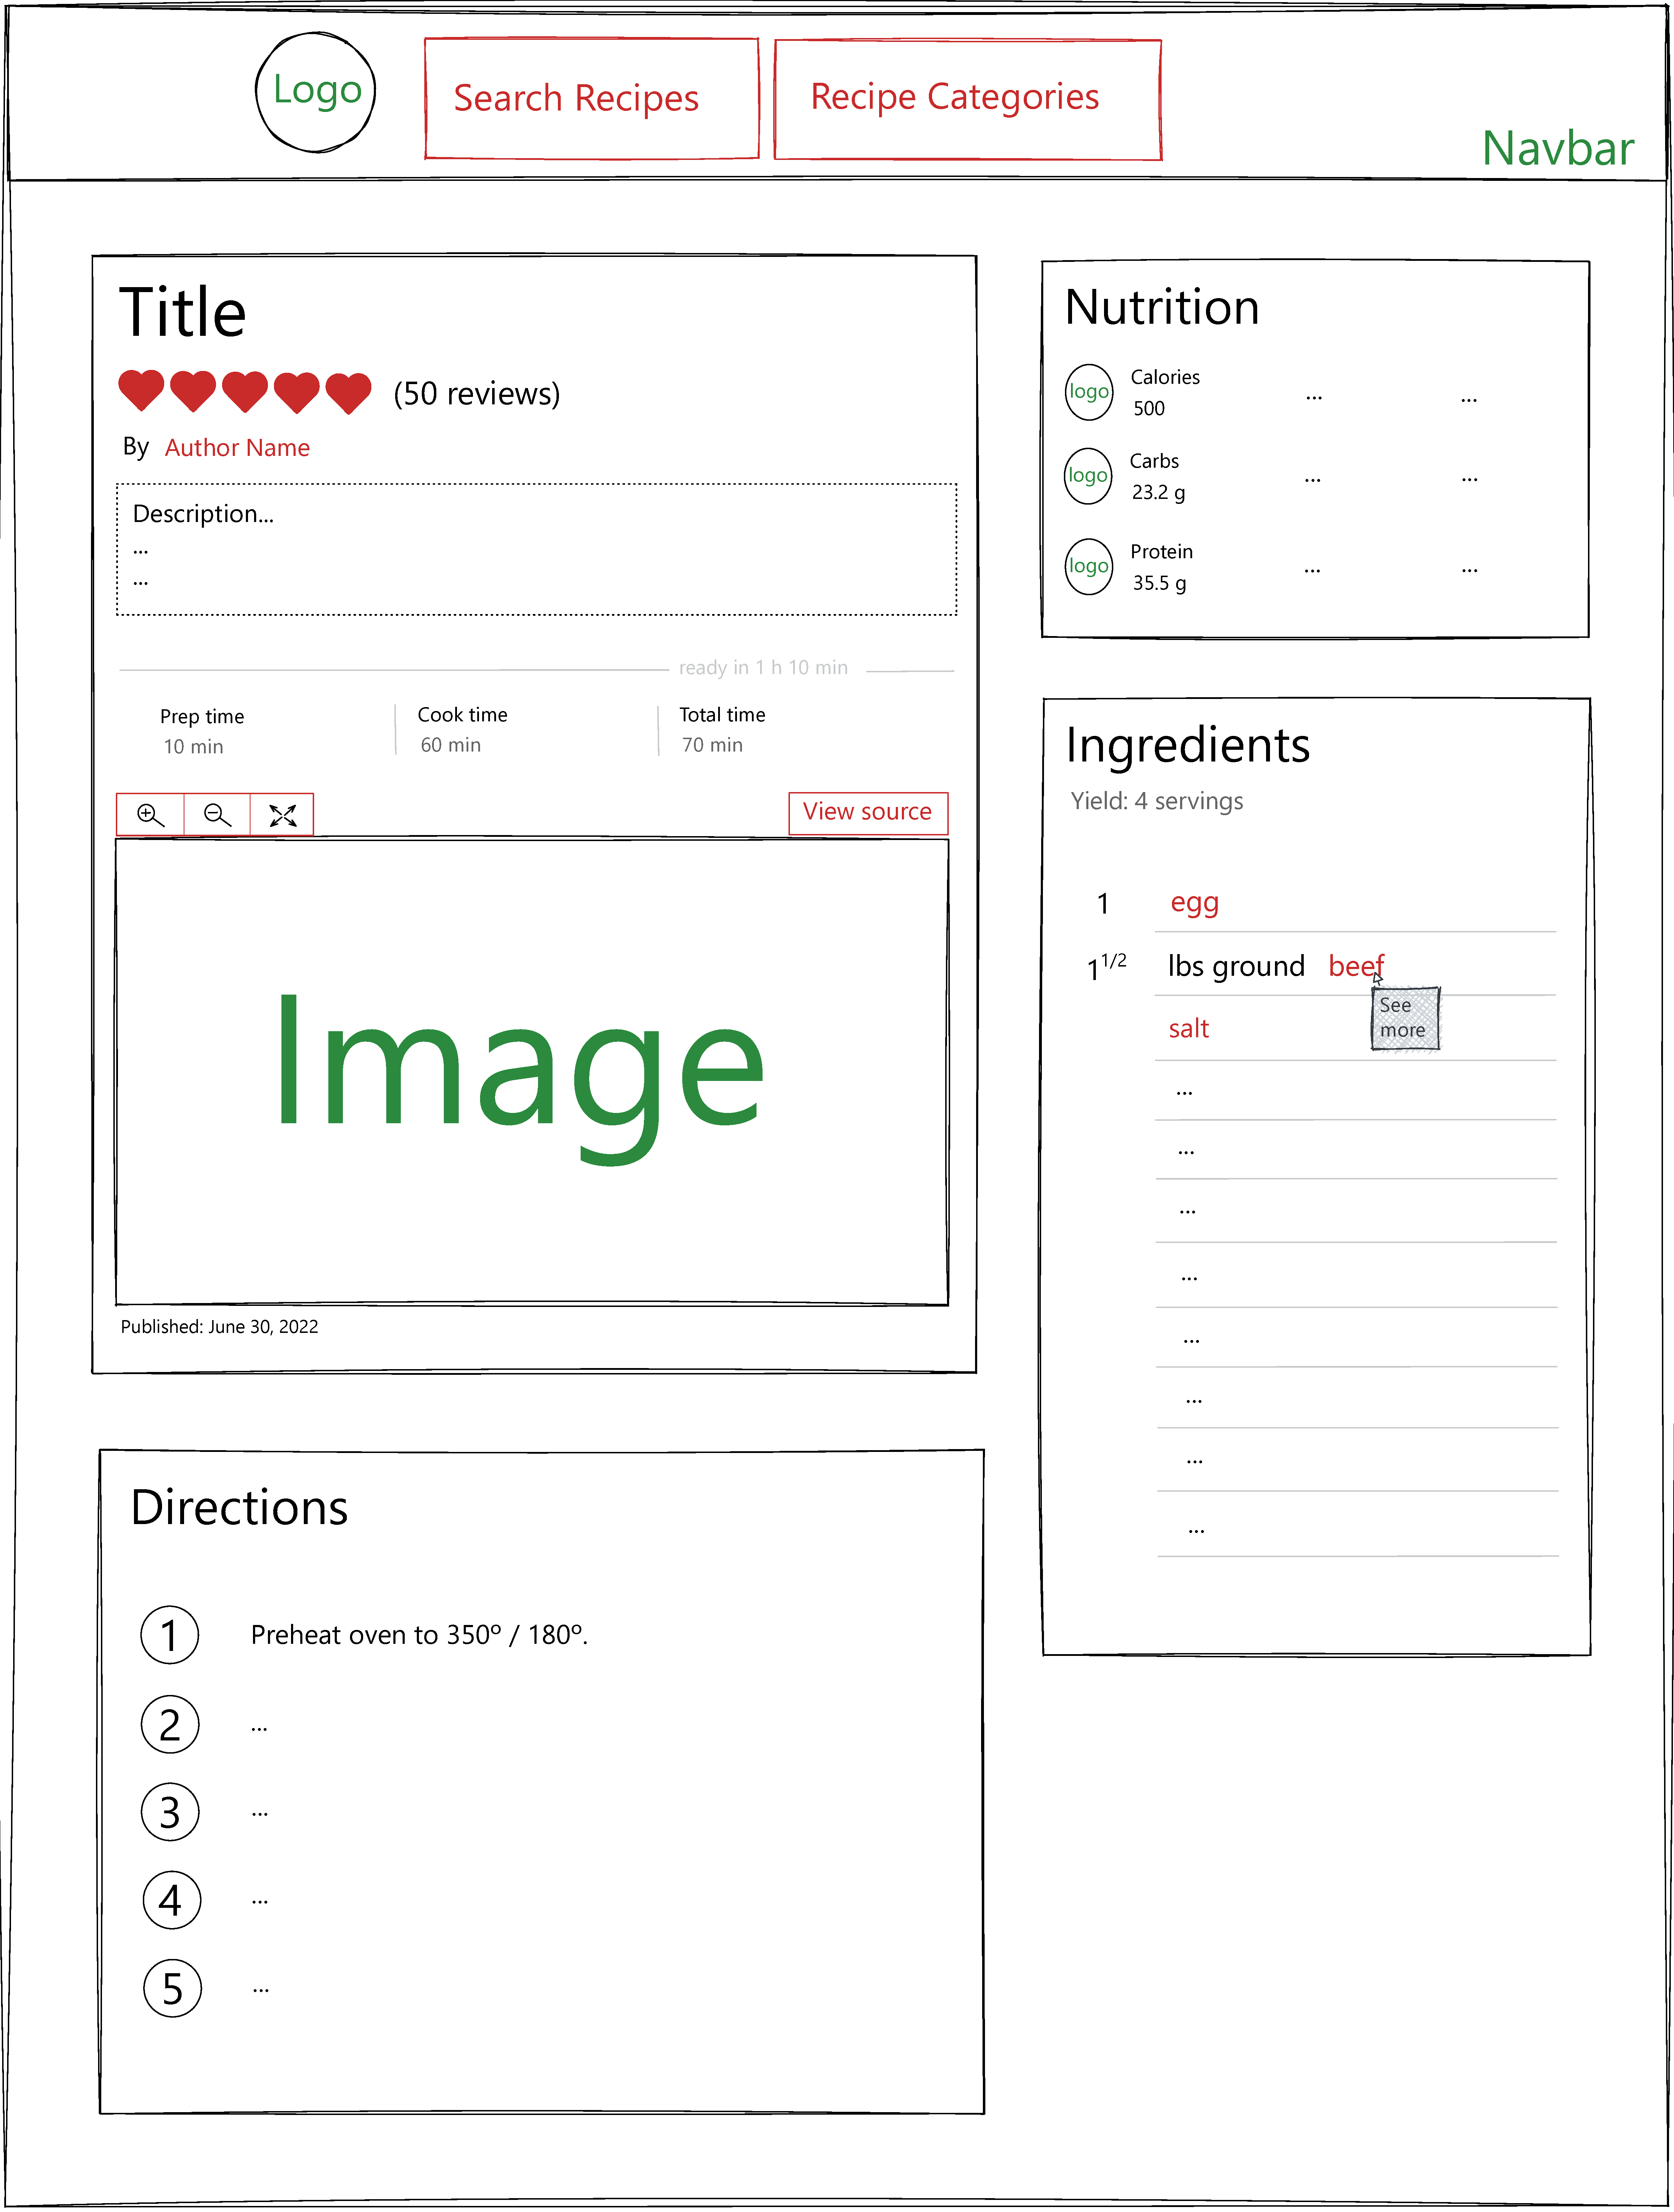
\includegraphics[width=140mm]{../img/detail-view}
\caption{Obrazovka detailu receptu.}
\label{obr02:detail-view}
\end{figure}

\subsubsection{Detail receptu}

Na obrazovce s~konkrétním receptem bude obsažen název, popis, obrázek, autor, datum publikování, hodnocení s~počtem recenzí, nutriční hodnoty a~samozřejmě ingredience a~postup přípravy. Rozložení pro větší obrazovky viz obrázek \ref{obr02:detail-view}, pro menší obrazovky se všechny karty zobrazí v $1$~sloupci analogicky k~rozložení \ref{obr02:mobile-search-view}. Jako budoucí rozšíření by bylo možné implementovat modul recenzí. V~první fázi by recenze byly pouze extrahovány ze zdrojových datasetů, v~další fázi by uživatelé mohli nové recenze přidávat prostřednictvím naší aplikace.

\subsubsection{Detail ingredience}

Na obrazovce detailu ingredience budou prezentována data z~otevřených znalostních grafů. Zaměříme se primárně na jméno, popis a~obrázek ingredience, které dle dostupných informací doplníme o~nutriční hodnoty, kategorie, místo původu a~další zajímavosti.

\subsection{Hierarchie komponent}

Se znalostí rozložení jednotlivých uživatelských obrazovek navrhneme příslušný systém komponent. Můžeme postupovat směrem od komponent s~největším dosahem, které odpovídají jedné obrazovce, ale také opačným směrem od komponent reprezentujících jednu základní část našeho datového modelu, například obrázek receptu. Snažíme se dodržovat princip jedné odpovědnosti a jakmile komplexita některé z~komponent začne příliš stoupat, provedeme dekompozici a~část práce přesuneme do komponenty potomka. Častým postupem je předání odkazu na funkci komponentě potomka. Funkce je pak zavolána jako callback například po stisknutí tlačítka, které je ve správě vnořené komponenty. Vztah předka a potomka bychom mohli přirovnat k~jeho pojetí v modelu DOM, kde by komponenty odpovídaly jednotlivým elementům, které lze do sebe vnořit. Nejedná se o~koncept dědičnost z~objektového návrhu, kde třída potomka vystupuje jako specializace třídy předka, musí splňovat všechny vlastnosti předka a~volitelně poskytovat dodatečné vlastnosti a~funkce.

\subsubsection{Kostra aplikace}

Kořenem našeho stromu komponent bude \texttt{BrowserRouter}, komponenta pocházející z~knihovny React Router. Ta bude obsahovat jedinou komponentu \texttt{App}, kterou dále rozdělíme na základní komponenty \texttt{Header}, \texttt{Routes} a~\texttt{Footer}. Komponenty \texttt{Header} a~\texttt{Footer} budou společné pro celou aplikaci, proto mohou být na úrovni komponenty \texttt{Routes}. Potomci komponenty \texttt{Routes} budou odpovídat jednotlivým obrazovkám, budeme tedy mít $3$ komponenty \texttt{Route} s~následujícími cestami provázanými s URL adresami:

\begin{code}
/recipes
/recipes/:recipeId
/ingredients/:ingredientId
\end{code}
%$

Části adres označené jako \texttt{:recipeId} a~\texttt{:ingredientId} značí proměnné, za které budou dosazeny konkrétní hodnoty přístupné skrze funkci \texttt{useParams} kni\-hovny React Router. Přidáme ještě dodatečnou komponentu \texttt{Route} pro zpracování domovské stránky, tedy s~cestou: \texttt{/}. Tato komponenta bude v~pilotní verzi naší aplikace pouze přesměrovávat na adresu \texttt{/recipes}. Grafické znázornění základní komponentové struktury aplikace viz schéma \ref{obr02:react-app}.

\begin{figure}[h!]\centering
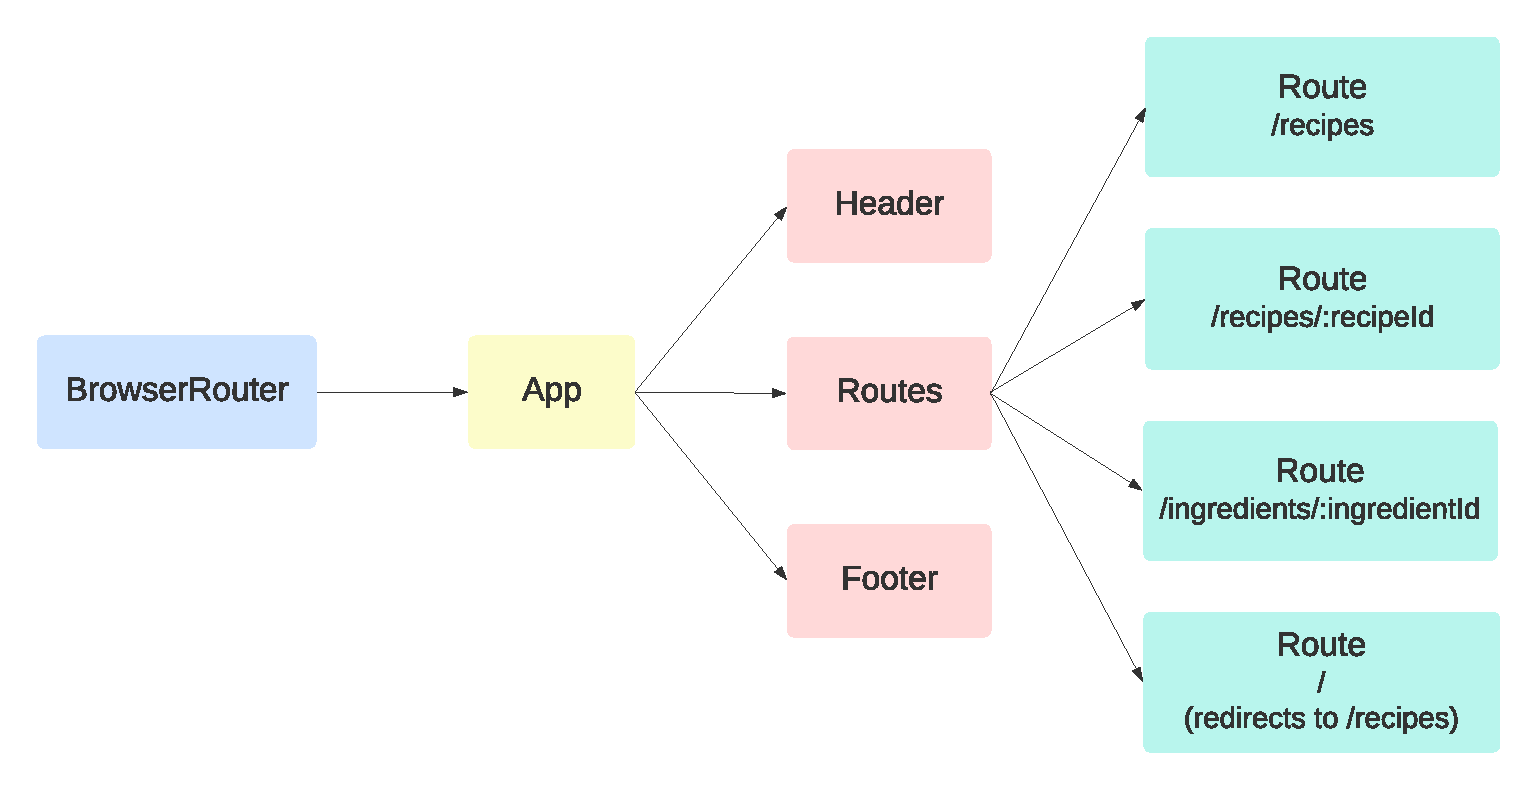
\includegraphics[width=140mm]{../img/react-app}
\caption{Rozhraní aplikace založené na konceptu knihovny React Router.}
\label{obr02:react-app}
\end{figure}

\subsubsection{Komponenta vyhledávání receptů}

Postup dekompozice si ukážeme na zjednodušeném převodu obrazovky pro vyhledávání receptů na komponenty knihovny React. Obsah celé vyhledávací obrazovky budeme reprezentovat komponentou \texttt{Recipes}. Ta bude zajišťovat mapování filtrů a~současné stránky prohlížení na query parametry URL adresy. Dále bude komunikovat s~REST API, konkrétně s~endpointem pro vyhledávání receptů \texttt{/api/recipes}. Výsledky receptů si vyžádá prostřednictvím asynchronního GET požadavku a~jakmile data obdrží, předá je specializovaným komponentám pro zajištění renderování. Těmito komponentami rozumíme potomky komponenty \texttt{Recipes}.

Jak bylo zmíněno v~začátku této sekce, potomci jsou vnořené komponenty, kterým lze předat data prostřednictvím parametru \texttt{props}. Příkladem vnořené komponenty bude \texttt{RecipesGrid}, která bude dále distribuovat informace o~receptech svým potomkům \texttt{RecipeCard}. Také komponenta \texttt{RecipeCard} bude složena z~menších komponent, konkrétně \texttt{RecipeCardContent}, \texttt{RecipeCardActions} a~\texttt{RecipeCardCollapse}. Rozhraní vyhledávaného receptu bude odpovídat schématu definovanému pro Solr, pojmenujme jej \texttt{SimpleRecipe} pro kontrast s~podrobnějším rozhraním receptu na stránce detailu. Diagram zachycující výše uvedené komponenty včetně parametrů \texttt{props} a~vzájemných vztahů je ilustrován obrázkem \ref{obr02:recipes-component}.

\begin{figure}[h!]\centering
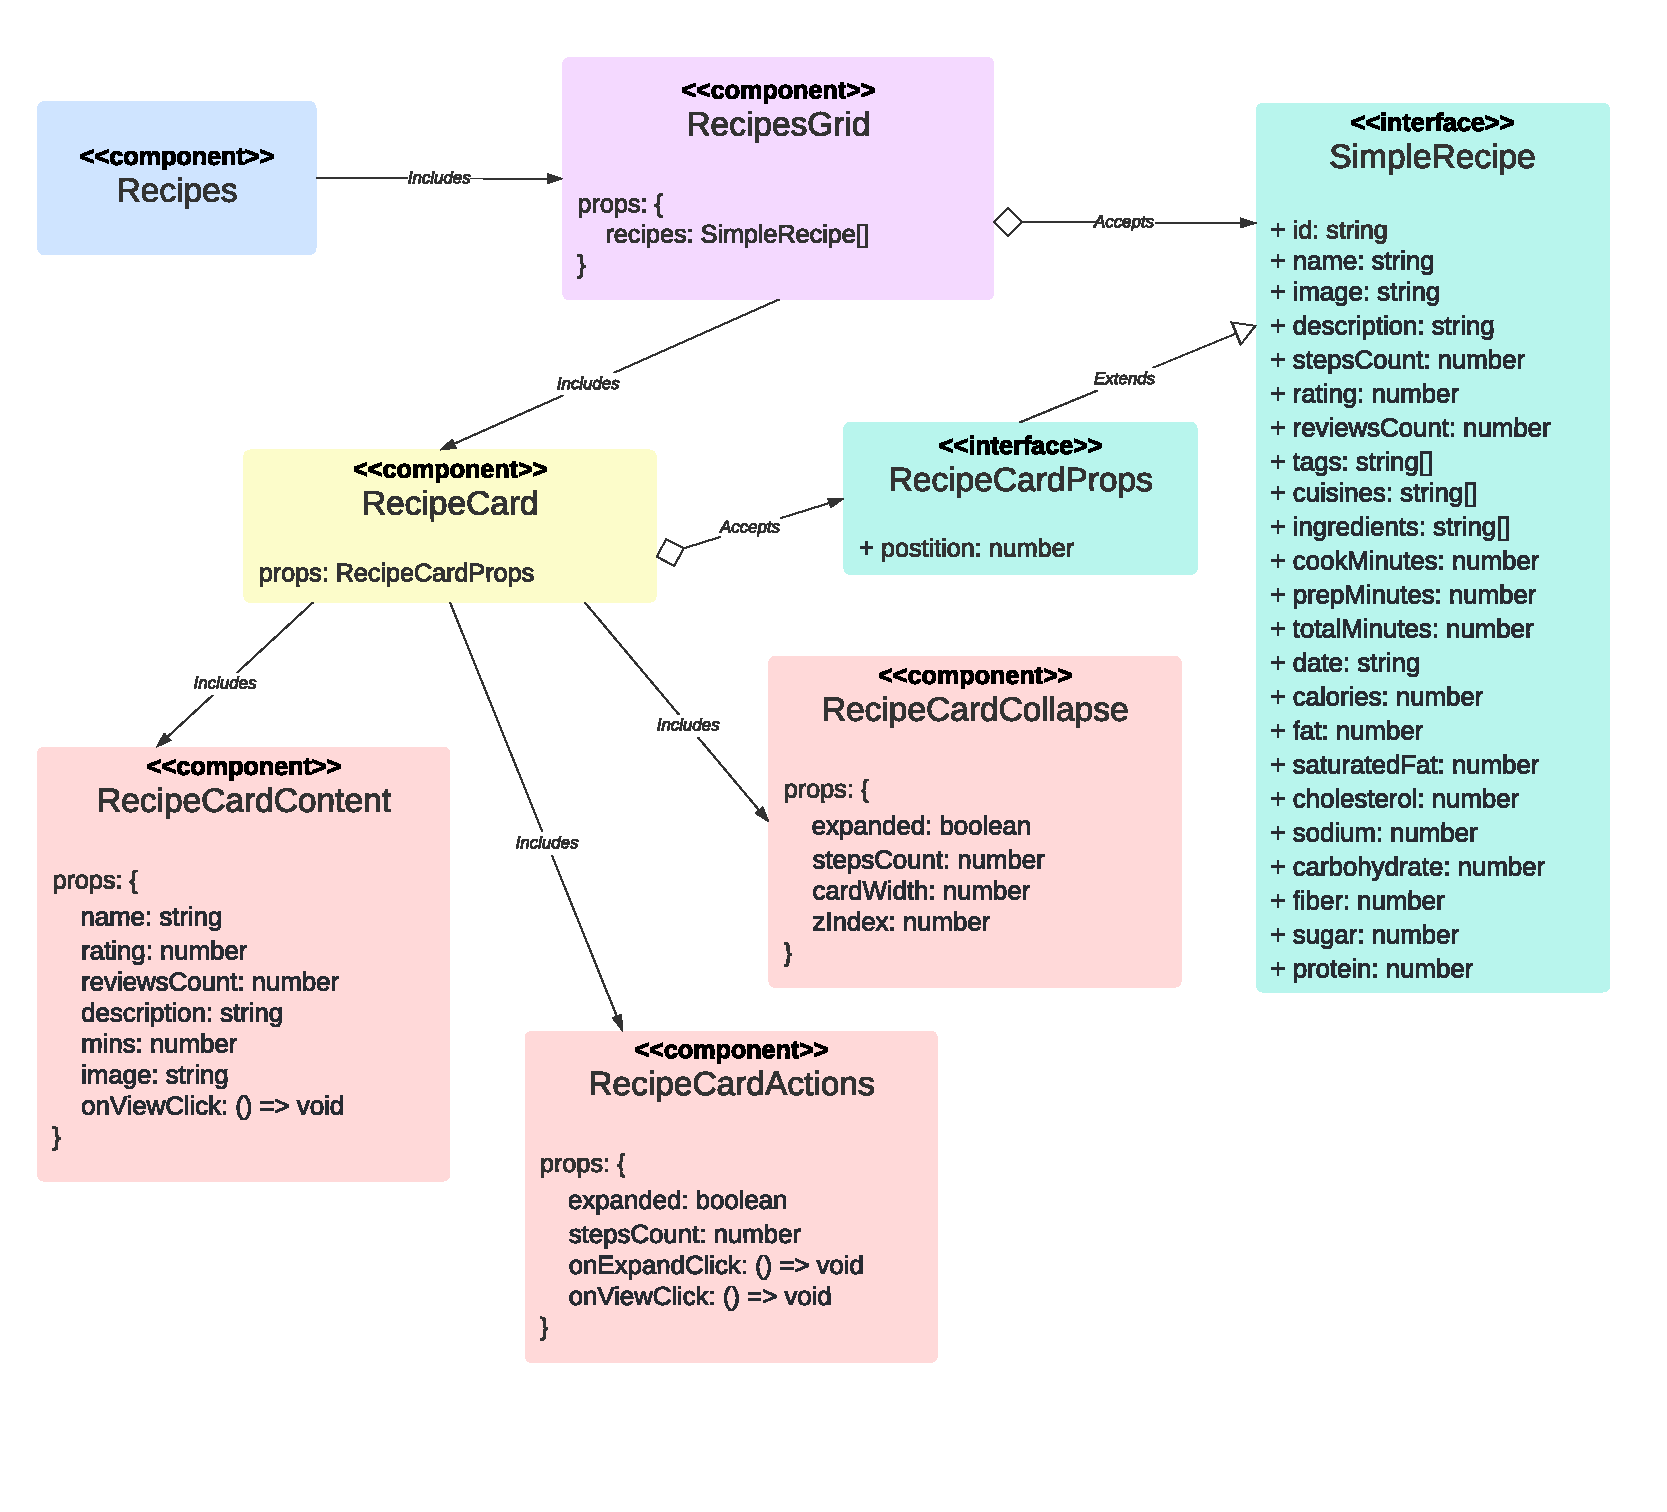
\includegraphics[width=145mm]{../img/recipes-component}
\caption{Diagram znázorňující dekompozici komponenty \texttt{Recipes}.}
\label{obr02:recipes-component}
\end{figure}

Komponenta \texttt{RecipeCardContent} se postará o~zobrazení obrázku, názvu receptu s~úryvkem popisu, hodnocení včetně počtu recenzí a~také času přípravy. Komponenta \texttt{RecipeCardActions} odpovídá spodnímu panelu karty receptu, se kterým lze interagovat. Je zde umístěné tlačítko pro zobrazení receptu a~také tlačítko pro rozbalení seznamu ingrediencí. Samotný seznam ingrediencí již není ve správě komponenty \texttt{RecipeCardActions}. Ta se jen stará o~jeho aktivaci, která je zajištěna zavoláním příslušné funkce předané jako parametr z~rodičovské komponenty \texttt{RecipeCard}. Proměnnou indikující stav rozbalení sekce s~ingrediencemi vlastní komponenta \texttt{RecipeCard}. Při zavolání funkce se tento stav změní a~komponenta \texttt{RecipeCard} předá novou hodnotu komponentě \texttt{RecipeCardCollapse}. Ta na základě aktualizované hodnoty zobrazí nebo skryje seznam ingrediencí.

Finální dekompozice komponenty \texttt{Recipes} bude samozřejmě o~něco složitější, neboť si kromě karet receptů musíme poradit také se zobrazením vyhledávacích filtrů, stránkováním a~nadpisem indikujícím aktuální stav vyhledávání. Rovněž budeme chtít uživatele informovat o~úspěšně přidaných nebo odstraněných filtrech prostřednictvím krátké notifikace. Během implementace uplatníme výše popsané principy dekompozice a~také se pokusíme v~co největší míře zapojit již hotové komponenty poskytované knihovnou Material UI.

\section{Alternativní správa dat}

Při návrhu architektury ukládání a~dotazování se nad daty receptů a~ingrediencí bychom se mohli vydat cestou konstrukce vlastního znalostního grafu. Museli bychom definovat ontologii, pomocí které bychom byli schopni kompletně popsat svou doménu receptů i~surovin. Sestrojený graf bychom nahráli do tzv.~\emph{RDF triplestore}, což je typ grafové databáze specializované na jednoduchá RDF tvrzení ve formátu trojic: \emph{subjekt}, \emph{predikát} a~\emph{objekt}. Vrcholy grafu jsou reprezentovány entitami subjektů a~objektů, orientované hrany mezi nimi modelujeme pomocí predikátů. Nad uloženými daty se lze následně dotazovat pomocí jazyka SPARQL, se kterým jsme se setkali při extrakci dat ze znalostních grafů DBpedia a~Wikidata.

\subsection{Projekt Linked Recipes}

Výše uvedený přístup byl otestován v~rámci souvisejícího projektu Linked \,Recipes\footnote{https://github.com/lhotanok/LinkedRecipes}, který vznikl jako semestrální práce v~předmětu Data na Webu vedeném RNDr.~Jakubem~Klímkem,~Ph.D. v~roce $2022$. Součástí projektu bylo získání dat s~recepty ze $3$~různých zdrojů, dále jejich převedení do RDF formátu v~libovolné serializaci, nalezení linků mezi datasety navzájem i~s~externími grafy a~na závěr vytvoření jednoduché aplikace, která všechna data propojila a~umožnila nad nimi spouštět SPARQL dotazy. Jako statické zdroje dat byly vybrány datasety Food.com Recipes and~Interactions a BBC Recipes. Ty byly obohaceny o~dataset vygenerovaný z~webové aplikace Allrecipes a~jako zástupci externích grafů byly zvoleny projekty DBpedia a~Wikidata. Je zde tedy velký překryv s~datovými sadami využívanými v~naší aplikaci pro vyhledávání receptů.

Aplikace Linked Recipes je napsána v~jazyce Java a~pro obsluhu HTTP požadavků využívá koncept tzv.~servletů, které generují odpovídající HTML dokumenty, často na základě komunikace s~databází. Aplikace používá RDF triplestore jako úložiště dat, konkrétně implementaci frameworku Eclipse RDF4J. Data ve formátu RDF jsou při spuštění aplikace nahrána do paměti prostřednictvím úložiště \emph{MemoryStore}, které je dle dokumentace třídy vhodné pro dataset s~méně než $100\,000$ tvrzeními. Alternativně lze použít úložiště provázané se SPARQL endpointem, který přijímá dotazy přes HTTP.

Aplikace si díky RDF triplestore a~SPARQL dotazům dokáže poměrně snadno poradit s~vyhledáním receptů dle ingrediencí, včetně zákazu vybraných ingrediencí. Také zvládá filtrovat recepty na základě povoleného rozmezí nutričních hodnot. Dalším v~aplikaci demonstrovaným příkazem je sestavení grafu ingrediencí s~využitím dat z~grafu Wikidata. Aplikace má k~dispozici seznam entit z~Wikidata, které se namapovaly na ingredience datasetů s~recepty. Přímo za běhu pak získává odkazy na obrázky k~daným ingrediencím a~vkládá je do HTML dokumentu. Nepotřebuje si tedy data k~ingrediencím z~Wikidata ukládat do interní databáze, čímž se zjednoduší architektura aplikace. Nevýhodou je ale podstatně delší čas potřebný k~získání a~zobrazení informací.

Pokud bychom se rozhodli pro stejný návrh aplikace jako v~projektu Linked Recipes, nahradili bychom vrstvy CouchDB a~Solr úložištěm RDF triplestore. To by v~sobě mělo uložena všechna data stejně jako CouchDB a~zároveň by řešilo vyhledávací dotazy namísto platformy Solr. Rychlost vyhledávání by byla závislá pouze na optimalizaci SPARQL dotazů. Narazili bychom na problém, pokud bychom se nespokojili s~vyhledáváním dle přesné shody a~vyžadovali chytřejší řešení po vzoru Solr a~jeho vyhledávání v~anglickém textu. Dále bychom se museli vypořádat s~požadavkem fasetového vyhledávání, pro které máme v~Solr přímou podporu na straně serveru. Fasetové vyhledávání se obvykle nepoužívá v~přímé kombinaci s~RDF modelem z~důvodu rizika, že by příkazy potřebné k~jeho podpoře byly příliš komplexní a~jejich výkon nedostačující \citep{sparql-facet}. Sehnat dostatečně výkonné a~dobře zdokumentované řešení by tedy bylo podstatně složitější v porovnání s~využitím osvědčeného Apache Solr nebo jeho alternativ v~podobě ElasticSearch\footnote{https://www.elastic.co/guide/en/app-search/current/facets-guide.html} či Sphinx\footnote{http://sphinxsearch.com/blog/2013/06/21/faceted-search-with-sphinx/}.
%%% Fiktivní kapitola s ukázkami tabulek, obrázků a kódu

\chapter{Implementace návrhu}

Před zahájením vývoje aplikace je potřeba nainstalovat všechny potřebné nástroje a~nakonfigurovat vývojové prostředí. Nejdůležitější nástroje, které vyžadují globální instalaci, jsou následující:

\begin{itemize}
    \item Node.js
    \item Python
    \item Docker
    \item Apache CouchDB
    \item Apache Solr
    \item Silk Workbench
    \item Apify CLI
\end{itemize}

V~řešení využijeme také řadu knihoven, které budeme instalovat pouze v~rámci projektu pomocí výchozího správce balíčků npm pro Node.js. Tyto knihovny vždy uvedeme na seznamu závislostí projektu, takže je lze snadno nainstalovat prostřednictvím příkazu \texttt{npm\,install}, případně ekvivalentního \texttt{yarn\,install}.

Co se týče výběru programovacích jazyků, přípravu dat vyřešíme pomocí vzájemně nezávislých skriptů psaných v~jazyce JavaScript. Samotnou aplikaci včetně serverové a~klientské vrstvy již napíšeme jazykem TypeScript, který je potřeba následně transpilovat do JavaScriptu. Tento dodatečný krok přidává komplexitu při spouštění kódu, proto jej vynecháme u~jednoduchých skriptů připravujících dokumenty pro databázi a~Solr. Zároveň ale přináší typovou kontrolu, kterou velmi oceníme v~komplexnější aplikaci a~to zejména při práci s~externími knihovnami, jejichž rozhraní není vždy perfektně zdokumentováno.

\section{Vývojové prostředí}

Aplikaci budeme vyvíjet v~editoru Visual Studio Code. Konzistentního formátování dosáhneme zapojením rozšíření Prettier\footnote{https://github.com/remimarsal/prettier-now-vscode}, které má na starosti správné odsazení, maximální délku řádky a~další aspekty formátování.

Projekt je verzován ve vzdáleném repozitáři na platformě GitHub pod jménem MeaLinker\footnote{https://github.com/lhotanok/MeaLinker}. Název byl sestaven spojením slov \emph{meal} a~\emph{linker}, snaží se totiž zachytit myšlenku propojení receptů z~různých zdrojů. Dosavadní práce probíhala pro zjednodušení ve větvi \texttt{main}. Pokud by se na projektu začalo podílet více vývojářů, byl by zaveden tradiční systém vedlejších větví pro implementaci jednotlivých funkcí a~požadavků na jejich sloučení s~hlavní větví.

\section{Zpracování vstupních dat}

Jak jsme již zmínili v~části o~architektuře aplikace, data k~receptům získáme primárně pomocí vlastní extrakce dat. Pro dataset z~webové aplikace Food.com využijeme i~statická data z~platformy Kaggle, kterými rozšíříme extrahované informace. Data k~ingrediencím ze znalostních grafů DBpedia a~Wikidata získáme rovněž automatizovaným postupem skrze zpracování HTTP požadavků.

Jako zdroje receptů jsme si zvolili webové aplikace Food.com a~Allrecipes. Pro každou z~nich vytvoříme dedikovaný extraktor s~využitím knihovny Apify. Nejprve se podíváme na řešení pro aplikaci Food.com, u~které nás na rozdíl od stránky Allrecipes čeká dodatečná fáze sloučení informací ze statického datasetu.

\subsection{Food.com}

Propojení dat se statickým datasetem Food.com Recipes and~Interactions do projektu vnáší poměrně velkou komplexitu ve srovnání s~pouhou extrakcí dat z~webové aplikace, kterou využijeme u~stránky Allrecipes. Pro zpracování dat z~aplikace Food.com nemůžeme využít stejný přístup jako s~Allrecipes, protože neposkytuje plně strukturované ingredience (odděluje pouze množství od ostatního textu). Výrazná výhoda zpracování dat z~Food.com je v~jejich kvantitě, která s~více než $500\,000$ recepty $10\times$ převyšuje aplikaci Allrecipes a~tvoří polovinu obsahu největšího datasetu s~recepty Recipe1M+. Také poskytuje detailní informace přibližně k~$900$ ingrediencím na adrese \texttt{food.com/about}. Tato data sice extrahovat nebudeme, počet ingrediencí s~detaily je pro nás ale užitečným vodítkem z~pohledu propojení s~otevřenými daty surovin.

Dataset Food.com Recipes and~Interactions obsahuje kolem $8\,000$ unikátních ingrediencí extrahovaných a~normalizovaných přímo z~jednotlivých receptů. Tyto normalizované ingredience budou po čištění velmi dobrým podkladem pro fasetový našeptávač ingrediencí na vyhledávací stránce. Využijeme je pro vyhledávání receptů z~libovolných zdrojů. Alternativně bychom mohli využít externí seznam ingrediencí, ať už z~aplikace Food.com nebo z~otevřených znalostních grafů. Počet navrhovaných přísad by ale byl výrazně menší.

\subsubsection{Extrakce dat}

Skripty pro přípravu dat z~aplikace Food.com jsou soustředěny v~adresáři \texttt{data/resources/foodcom}. Samotná logika extrakce dat je umístěna v podadresáři \texttt{food-com-scraper}, jehož struktura odpovídá standardnímu Apify actorovi představenému v~předchozí kapitole. Pro vytvoření této struktury lze využít příkaz \texttt{apify\,create}, který uživatele provede možnostmi různých šablon. My zvolíme šablonu pro tzv. \texttt{CheerioCrawler}, což je v~knihovně Apify řešení využívající HTTP požadavky a~parsování HTML z~odpovědi. Pokud bychom potřebovali automatizaci webového prohlížeče, použili bychom šablonu \texttt{PuppeteerCrawler}, případně \texttt{PlaywrightCrawler}. Šablony jsou pojmenovány podle klíčových technologií, tedy knihovny Cheerio pro extrakci dat z~HTML a~knihoven Puppeteer či Playwright poskytujících rozhraní pro automatizaci prohlížeče.

Pokud bychom adresář s~Apify actorem například naklonovali ze vzdáleného adresáře na platformě GitHub, stačilo by jej inicializovat příkazem \texttt{apify\,init}. Zároveň se jedná o~standardní Node.js projekt, musíme tedy nainstalovat všechny závislosti uvedené v~souboru \texttt{package.json}. Po inicializaci se vytvoří důležitý adresář \texttt{apify\underline{{ }}storage} s~podadresáři \texttt{datasets} a~\texttt{key\underline{{ }}value\underline{{ }}stores}.

Do adresáře \texttt{datasets} se typicky ukládají JSON soubory s~jednotlivými položkami datasetu, v~našem případě recepty. Na cloudové platformě Apify se pak tyto soubory sloučí do společného datasetu, který lze stáhnout v~řadě různých formátů, z~nichž nejčastěji využívané jsou formáty JSON a~CSV. Naše řešení bude ale určeno pouze pro lokální vývoj, pro zjednodušení tedy budeme výsledky ukládat přímo sloučené do adresáře \texttt{key\underline{{ }}value\underline{{ }}stores/default} pod klíčem \texttt{RECIPES}. Zároveň zde pod klíčem \texttt{INPUT} najdeme další důležitý soubor se vstupem pro actora. Ten bude obsahovat objekt s~jedinou položkou \texttt{startUrls} v~následujícím formátu:

\begin{code}
{
  "startUrls": [
    {
      "url": "https://www.food.com/recipe/219662"
    },
    {
      "url": "https://www.food.com/recipe/103336"
    }
  ]
}
\end{code}
%$

Vstup bude vygenerován do \texttt{key\underline{{ }}value\underline{{ }}stores/defalut/INPUT.json} pomocí skriptu \texttt{recipe-urls-generator.js} z~adresáře \texttt{foodcom}, který URL adresy složí z~identifikátorů receptů. Před spuštěním tohoto skriptu je potřeba mít staženy soubory \texttt{recipes/RAW\underline{{ }}recipes.csv} a~\texttt{recipes/PP\underline{{ }}recipes.csv} z~datasetu Food.com Recipes and~Interactions\footnote{https://www.kaggle.com/datasets/shuyangli94/food-com-recipes-and-user-interactions} a~dokončen \texttt{recipes-preprocessing.js}. Přes proměnnou \texttt{RECIPES\underline{{ }}TO\underline{{ }}EXTRACT} uvnitř \texttt{constants.js} lze omezit počet receptů, které se mají extrahovat.

Kód Apify actora je typicky soustředěn v~adresáři \texttt{src}. Klíčové jsou soubory \texttt{main.js} s~inicializací (v našem případě třídy \texttt{CheerioCrawler}) a~\texttt{routes.js} s~funkcemi pro zpracování různých typů obrazovek. Obvykle je potřeba definovat chování pro stránku typu \texttt{LIST}, ze které jsou získány odkazy na detaily nalezených výsledků, a~pro stránku \texttt{DETAIL}, kde jsou extrahována a~uložena data jednotlivých výsledků. Naše řešení pro aplikaci Food.com zpracovává pouze detaily receptů, které obdrží na vstupu. Stačí tedy implementovat funkci \texttt{handleDetail}, která pomocí CSS selektoru \texttt{script[type="application/ld+json"]} zacílí JSON-LD data z~hlavičky HTML dokumentu, vybranou část z~nich převede do strukturované podoby a~nově zkonstruovaný recept přidá do souboru \texttt{RECIPES.json}.

Konstruktor třídy \texttt{CheerioCrawler} přijímá $1$ parametr s~možnostmi konfigurace. Prostřednictvím položky \texttt{proxyConfiguration} lze volitelně aktivovat rotování IP adres, které chrání naši vlastní IP adresu před dočasným či dokonce trvalým zablokováním a~zlepšuje poměr úspěšných požadavků. Vzhledem k~obecně nižší míře blokování ze strany aplikací s~recepty by využití proxy nemělo být nutné, je ale vhodné. Pro využití automatické proxy je potřeba přihlášení do Apify účtu s~dostupnými proxy adresami. Také lze poskytnout vlastní proxy. Počet současně odesílaných požadavků omezíme na doporučenou hranici $50$ požadavků, abychom zamezili přetížení zpracovávané webové aplikace. Actora spustíme příkazem \texttt{apify\,run\,-p}. Příznak \texttt{-p} je zkratkou pro \emph{purge} a~zajišťuje korektní vyčištění předchozího stavu.

\subsubsection{Propojení dat}

V~první fázi potřebujeme extrahovat ingredience, které jsou poskytnuty v~souboru \texttt{ingr\underline{{ }}map.pkl}. Pro zpracování formátu \emph{pkl} potřebujeme knihovnu pickle určenou k~serializaci a~de-serializaci objektů jazyka Python \citep{pickle}. Je tedy potřeba aktivovat prostředí pro vývoj v~jazyce Python s~nainstalovaným balíčkem pickle (typicky virtuální prostředí označované jako \emph{venv}). Soubor převedeme skriptem \texttt{pkl-ingredients-extractor.py} do formátu CSV, kde nalezneme informace v~následujícím formátu:

\begin{code}
raw_ingr,raw_words,processed,len_proc,replaced,count,id
romaine lettuce leaf,3,romaine lettuce leaf,20,lettuce,4507,4308
iceberg lettuce leaf,3,iceberg lettuce leaf,20,lettuce,4507,4308
red romaine lettuce,3,red romaine lettuce,19,lettuce,4507,4308
\end{code}
%$

Klíčové pro nás budou unikátní hodnoty ze sloupců \texttt{replaced} a~\texttt{id}, přičemž každá hodnota \texttt{replaced} má přiřazeno unikátní \texttt{id}. Jména surovin normalizujeme na přísady pro vyhledávání pomocí skriptu \texttt{ingredients-preprocessing.js}. Dále z~nich vytvoříme jednoduchý RDF dataset ve formátu Turtle prostřednictvím skriptu \texttt{rdf-data/rdf-ingredients-converter.js} a~tento dataset nahrajeme do aplikace Silk Workbench pro nalezení linků s~grafy DBpedia a~Wikidata.

Normalizované názvy ingrediencí přidáme do receptů extrahovaných Apify actorem, což provedeme na základě informací ze souboru \texttt{RAW\underline{{ }}recipes.csv}, kde jsou propojeny recepty s~identifikátory ingrediencí. Stejným způsobem přidáme informace o~autorovi včetně jeho id. Tuto fázi má na starosti hlavní skript pro slučování dat, totiž \texttt{recipes-ingredients-merge-manager.js}.

Poslední fáze patří skriptu \texttt{ingredients-postprocessing.js}, který v~adresáři \texttt{rdf-data} očekává soubor \texttt{dbpedia-ingredients.json} s~extrahovanými ingrediencemi z~grafu DBpedia a~soubor \texttt{wikidata-ingredients.json} s~přísadami z~Wikidata. Ty generuje skript \texttt{rdf-data/external-dataset-linker.js}, který potřebuje soubory v~RDF formátu N-triples \texttt{rdf-data/dbpedia-links.nt} a~\texttt{rdf-data/wikidata-links.nt} vytvořené pomocí Silk Workbench. Konfigurace linkování extrahovaná z~grafického rozhraní Silk Workbench je uložena v XML souborech ve stejném adresáři.

Výstupem našeho řetězce zpracování jsou následující soubory:
\begin{code}
recipes/extended_recipes.json
ingredients/extended_ingredients.json
ingredients/search_ingredients.json
\end{code}
%$
První $2$~uvedené soubory jsou určeny pro uložení do databáze CouchDB a~poslední soubor najde uplatnění při tvorbě fasetových ingrediencí receptů uložených v~Solr. Skripty pro jednotlivé fáze zpracování jsou soustředěny v souborech \texttt{run} a \texttt{run-venv} vyžadující aktivované prostředí pro vývoj v~Pythonu.

\subsection{Allrecipes}

Pomocí vlastní extrakce dat získáme kompletní sadu receptů z~webové aplikace Allrecipes. Vyřadíme pouze recepty, které neobsahují informace o~nutričních hodnotách. Základní struktura actora pro extrakci dat z~Allrecipes bude podobná jako u~Food.com v~předchozí sekci. Speciálně zpracování stránek s~detaily receptů bude téměř identické, pouze využijeme dodatečné informace k~ingrediencím obsažené v~HTML elementech a~uložíme je na pozici strukturovaných ingrediencí. Mezi actory ale bude podstatný rozdíl v~získání odkazů na jednotlivé recepty. Actor pro Allrecipes nebude URL adresy přijímat na vstupu a namísto toho si je vyrobí sám. Má více způsobů, jak k~extrakci přistoupit. My se podíváme na extrakci prostřednictvím interního API z~vyhledávací stránky receptů a~na typický přístup procházení jednotlivých kategorií.

\subsubsection{Interní API}

Při vyhledávání receptů na základě filtrů můžeme přes vývojářské nástroje webového prohlížeče odchytit požadavek v~následujícím formátu:

\begin{code}
/element-api/content-proxy/faceted-searches-load-more?page=1
\end{code}
%$
Formát odpovědi na tento požadavek je následující:
\begin{code}
{
    hasNext: boolean
    html: string
    totalResults: number
}
\end{code}
%$

Ze znalosti hodnoty {totalResults} a~počtu výsledků na $1$~stránce bychom měli být schopni předem určit, kolik stran budeme procházet. V~době psaní této práce je inzerovaný počet výsledků uložený v~položce \texttt{totalResults} roven $55\,680$. Poslední stranou při číslování od $1$~by tedy měla být strana $2\,320$. Při manuální kontrole lze ale zjistit, že poslední výsledky jsou na straně $417$, kde je zároveň uloženo \texttt{hasNext:\,false}.

Lze tedy předpokládat, že pokud na Allrecipes zadáme prázdnou množinu filtrů a~prolistujeme všechny výsledky, neuvidíme inzerovaných $55\,680$ receptů, ale pouhých $(416 \cdot 24) + 16 = 10\,000$. Při podrobnějším zkoumání vypozorujeme, že aplikace Allrecipes používá maximální limit $10\,000$ výsledků i~při zadání filtrů (například po přidání soli jakožto vyhledávací ingredience se celkový počet výsledků snížil na necelých $40\,000$ a~poslední stranou výsledků je opět strana $417$. Pokud se tedy nespokojíme s $10\,000$ recepty, budeme muset přistoupit na řešení procházející jednotlivé kategorie receptů.

\subsubsection{Kategorie receptů}

Odkazy na kategorie je možné získat ze stránky s~relativní adresou \texttt{/recipes} přes CSS selektor třídy \texttt{recipeCarousel\underline{{ }{ }}link}. Kategorie pak můžeme procházet po stranách, stačí přidat query parametr \texttt{page}. Příklad relativní adresy pro $10$. stránku kategorie hlavních chodů: \texttt{/recipes/80/main-dish/?page=10}. Tento formát lze objevit při prozkoumání atributů tlačítka \texttt{Load\,more} na domovské stránce kategorie. Zda jsme již dorazili na poslední stranu poznáme podle obsahu elementu \texttt{h1}, ve kterém se na stránce bez receptů objeví hlášení \texttt{Page\,Not\,Found}.

Stránky kategorií budou v~kontextu Apify actora odpovídat stránkám typu \texttt{LIST}. V~rámci zpracování stránky kategorie musíme do fronty požadavků zařadit odkaz na další stranu a~zároveň URL adresy detailů receptů. Fronta je oboustranná, můžeme tedy adresy s~detaily receptů zařadit na začátek, aby se zpracovaly přednostně a~měli jsme dříve k~dispozici výsledky. Recepty se totiž průběžně ukládají do souboru \texttt{key\underline{{ }}value\underline{{ }}stores/default/RECIPES.json}.

Během extrakce dat ze stránek detailů receptů se musíme vypořádat s~několika problémy. Aplikace Allrecipes není zcela konzistentní v~mapování ingrediencí na atributy v~HTML a~střídá obsah $2$~atributů souvisejících se jménem ingredience. Tyto atributy vyjadřují:
\begin{itemize}
    \item Jméno ingredience zobrazované uživateli.
    \item Název ingredience určený pro vyhledávání.
\end{itemize}
Musíme tedy explicitně zkontrolovat, že pod položkou \texttt{text} ukládáme skutečně text, který je uživateli zobrazen bezprostředně po jednotce měření. Také narazíme na část receptů bez uvedených nutričních hodnot. Tyto recepty přeskočíme, neboť je pro nás informace o~nutričních hodnotách důležitá.

\subsubsection{Propojení dat}

U~datasetu z~Allrecipes máme zjednodušenou práci, neboť strukturované ingredience máme již k~dispozici z~fáze extrakce receptů. Stačí nám tedy získat unikátní jména ingrediencí z~extrahovaných receptů, z~těchto ingrediencí vytvořit RDF dataset pro linkování s~grafy DBpedia a~Wikidata a~extrahované informace propojit s~dokumenty receptů. Postup je analogický jako s~unikátními ingrediencemi z~Food.com datasetu. 

Ingrediencím potřebujeme přiřadit identifikátor a~ideálně se budeme snažit vyhnout duplicitě s~ingrediencemi z~Food.com, až je budeme ukládat do databáze spolu s~rozšířením z~DBpedia a~Wikidata. Vygenerujeme si tedy uuid pro celou naši aplikaci, které budeme využívat jako tzv.~\emph{seed} pro vytvoření dalších identifikátorů. Zde se nám bude hodit knihovna \texttt{uuid}\footnote{https://www.npmjs.com/package/uuid} a~její funkce \texttt{v5}:
\begin{code}
uuid.v5(name.toLowerCase(), NAMESPACE_UUID)
\end{code}
%$
Pokud takto vytvoříme identifikátory surovin stejného jména, namapují se na stejné uuid a vyhneme se duplicitě.

\subsection{Linkování se znalostními grafy}

Pro nalezení linků mezi ingrediencemi z~našich datasetů a~entitami z~DBpedia a~Wikidata využijeme nástroj Silk Workbench, pomocí kterého vytvoříme RDF tvrzení s~IRI adresami ingrediencí spojenými vztahem \texttt{owl:sameAs}. V~rámci úlohy linkování navrhneme transformaci textu ingrediencí, která dokáže názvy propojit i~s~mírnými odlišnostmi ve formátu, čísle nebo pádu slov. Grafické znázornění jednotlivých fází transformace viz \ref{obr0a:silk-workbench}, příslušné XML soubory pro spuštění přes příkazovou řádku jsou pro Food.com i~Allrecipes v~adresáři \texttt{rdf-data}.

\subsection{DBpedia}

Podklady pro extrakci dat ze znalostního grafu DBpedia jsou umístěny v~adresáři \texttt{data/resources/dbpedia}. Přiložený skript není určen pro samostatné spouštění, pouze poskytuje rozhraní pro skripty konkrétních datasetů uvnitř podadresářů \texttt{rdf-data}. Před zahájením extrakce vždy nejprve identifikujeme entity, ke kterým potřebujeme zjistit dodatečné informace. Jakmile máme IRI adresy připraveny, teoreticky bychom mohli vytvořit jeden společný SPARQL dotaz pro všechny entity a~ten odeslat na DBpedia SPARQL endpoint. Dotaz by ale mohl skončit příliš dlouhý a~nenechal by prostor pro škálování.

Zvolíme tedy alternativní řešení --- dynamicky vytvoříme sadu dotazů stejného formátu, každý s~přibližně $5$ IRI adresami. Počet adres musí zůstat nízký, neboť praktický test ukázal, že se jinak nevrátí všechny požadované výsledky. Dotazy zpracujeme paralelně a~výsledky uložíme do společného JSON datasetu. Šablona dotazu konstruujícího RDF graf je v~souboru \texttt{ingredients-dbpedia.sparql}. IRI adresy ingrediencí jsou pomocí regulárních výrazů vkládány do množiny \texttt{VALUES}. Dotaz ve zjednodušené podobě vypadá následovně:

\begin{code}
PREFIX rdfs: <http://www.w3.org/2000/01/rdf-schema#>
PREFIX dbo: <http://dbpedia.org/ontology/>
PREFIX dbp: <http://dbpedia.org/property/>

CONSTRUCT {
    ?ingredient rdfs:comment ?comment ;
                rdfs:label ?label ;
                dbo:thumbnail ?thumbnail ;
}
WHERE {
    VALUES ?ingredient { 
        ##INGREDIENTS## 
        # Replace this section with ingredient resources such as:
        # <http://dbpedia.org/resource/Avocado>
        ##INGREDIENTS##
    }

    # Label is the only required property
    ?ingredient rdfs:label ?label .
    FILTER (LANG(?label) = "en")
    
    OPTIONAL {
        ?ingredient rdfs:comment ?comment .
        FILTER (LANG(?comment) = "en")
    }

    OPTIONAL {?ingredient dbo:thumbnail ?thumbnail .}
}
\end{code}
%$

Výsledky si navíc od SPARQL endpointu můžeme vyžádat v~řadě různých formátů. Pro naše účely bude nejpraktičtější formát JSON-LD, jehož obsah využijeme v~hlavičkách HTML dokumentů. Se SPARQL endpointem lze komunikovat přes grafické rozhraní ve webovém prohlížeči nebo prostřednictvím HTTP GET požadavků. Pro snadnější automatizaci procesu extrakce využijeme druhou možnost, kde obsah dotazu předáme na místě query parametru s~názvem \texttt{query}. 

\subsection{Wikidata}

Proces extrakce dat z~grafu Wikidata bude probíhat analogicky k~postupu pro DBpedia z~předchozího odstavce. I~zde využijeme HTTP GET požadavky na SPARQL endpoint, kde prostřednictvím query parametrů předáme obsah dotazu a~požadovaný formát výsledku. Projekt Wikidata neposkytuje reprezentaci JSON-LD, vystačíme si ale s~běžným JSON formátem, který lze vyžádat přes hodnotu query parametru \texttt{format} nastavenou na \texttt{json}. Z~této reprezentace pak sami vytvoříme odpovídající JSON-LD formát, který je vhodný pro strukturovaná data v~hlavičce HTML dokumentu.

Související soubory jsou uloženy v~destinaci: \texttt{data/resources/wikidata}. Obsažený skript je opět volán pouze externě na základě extrahovaných ingrediencí z~datasetů Food.com a~Allrecipes. 

\section{Databáze Apache CouchDB}

Pro uložení dat jsme vybrali dokumentový databázový systém CouchDB z~důvodů popsaných v~kapitole o~architektuře aplikace.  S~CouchDB můžeme komunikovat přes webové rozhraní skrze aplikaci Fauxton, pomocí REST~API nebo prostřednictvím již zmíněné knihovny v~prostředí Node.js. Pro automatizované nahrávání dokumentů využijeme oficiální knihovnu Nano\footnote{https://www.npmjs.com/package/nano}.

S~velikostí našeho projektu si můžeme dovolit při nahrávání nových dat nejprve stávající data odstranit a~poté je vložit do čisté databáze. Kdybychom totiž chtěli dokumenty aktualizovat, potřebovali bychom u~každého z~nich poskytnout aktuální verzi, což by pro přepsání celé databáze byl zbytečně komplikovaný postup. Proces ale musíme paralelizovat, neboť již pro přidání kolekce o~velikosti $50\,000$ dokumentů se při sériovém řešení pohybujeme v~řádu delších minut.

S~knihovnou Nano pracujeme na $2$~místech projektu. Poprvé v~rámci přípravy a~nahrání dat do CouchDB, podruhé na backendu aplikace pro získání uložených dokumentů na základě identifikátorů. Oba přístupy do databáze vyžadují přihlašovací heslo --- uložíme jej jako proměnnou prostředí, ke které se v~kódu dostaneme přes rozhraní \texttt{process.env}. Instanci CouchDB spustíme na výchozím portu $5984$.

\subsection{Vložení dokumentů}

Nahrávání dokumentů zajišťuje skript \texttt{database-manager.mjs} umístěný v~adresáři \texttt{data/database}. Před uložením dokumentů do databáze jsou všechny řetězce obsažené v~jednotlivých objektech receptů a~ingrediencí dekódovány pomocí funkcí \texttt{decode} a~\texttt{unescape} z~knihoven \texttt{html-entities} a~\texttt{html-escaper}.

\subsection{Přístup k~dokumentům}

Kód pro hledání dokumentů receptů a~ingrediencí dle zadaného id je soustředěn v~adresáři \texttt{app/backend/src/couchdb}. Dokumenty jsou rozděleny do databází, respektive kolekcí \texttt{recipes} a~\texttt{ingredients}. Adresář \texttt{types} obsahuje definice, které potřebujeme pro typovou podporu jazyka TypeScript a~odpovídajícího IntelliSense. Schéma dokumentů není pevně definováno, takže typy slouží spíše pro naši kontrolu a~případné logování. Zejména na backendu aplikace, kde s~jednotlivými položkami objektů většinou nepotřebujeme dále pracovat a~nezměněný objekt odesíláme na frontend. Stejnou kolekci typů definujeme zvlášť na backendu i~frontendu, neboť by jejich adresáře teoreticky mohly být uloženy na různých zařízeních a~tudíž by na sobě neměly být závislé. Pokud by nám vzájemná závislost nevadila, stačilo by vytvořit typy pouze jednou v~kořenovém adresáři \texttt{app}, do kterého mají přístup obě části aplikace. Aktuálně se v~kontextu databáze jedná o~typy \texttt{FullRecipe}, \texttt{FullIngredient}, \texttt{RecipeJsonld} a~řadu vnořených typů, například \texttt{RecipeIngredient}, \texttt{RecipeNutrition}, \texttt{PrepTime} nebo \texttt{Author}. 

Spojení s~databází inicializujeme pouze jednou, což zaručíme zapojením třídy \texttt{NanoDbFactory} a~konceptu návrhového vzoru singleton. Odkaz na spojení s~databází si vždy vyžádáme od \texttt{NanoDbFactory}, která spravuje statický slovník spojení dle jména kolekce, v~našem případě \texttt{recipes} a~\texttt{ingredients}. Pokud už má pro dané jméno spojení navázáno, nevytváří jej znova a~vrátí odkaz na hodnotu ze slovníku. Se třídou \texttt{NanoDbFactory} komunikují modely dokumentů receptů a~ingrediencí, tedy třídy \texttt{CouchDbRecipesModel} a~\texttt{CouchDbIngredientsModel}. Pro každý zpracovávaný požadavek ze strany klienta se tak vytváří nová instance modelu, ale nikoli nové spojení s~databází.

\section{Vyhledávání pomocí Apache Solr}

Stejně jako u~práce s~databází můžeme komunikaci se Solr rozdělit do $2$~fází:
\begin{itemize}
    \item Příprava dokumentů.
    \item Zpracování dotazů nad dokumenty.
\end{itemize}

V~obou fázích využijeme knihovnu Solr client\footnote{https://www.npmjs.com/package/solr-client}, která implementuje veškerou komunikaci se Solr potřebnou pro splnění požadavků aplikace. S~platformou Solr bychom se dorozuměli i~prostřednictvím jejího REST~API, což využijeme při tvorbě schématu. Pro vkládání dokumentů a~dotazování se nad nimi je ovšem pohodlnější pracovat s~více high-level rozhraním, což nám umožní právě zmíněná knihovna.

\subsection{Příprava dokumentů}

Během tvorby schématu pro dokumenty receptů musíme zohlednit $2$~základní požadavky vyhledávání:
\begin{itemize}
    \item Vyhledávané termíny musí být analyzovány jako lokalizovaný text, aktuálně výhradně anglický.
    \item Během vyhledávání musí být k~dispozici našeptávač s~fasetovou hierarchií filtrů.
\end{itemize}

\subsubsection{Podpora fasetového vyhledávání}

Platforma Solr poskytuje přímou podporu fasetové navigace nad libovolnými položkami dokumentů. Můžeme tedy například snadno specifikovat fasetové vyhledávání nad ingrediencemi, čímž získáme list unikátních jmen surovin, které se v~celé kolekci receptů vyskytují. Je zde ovšem jisté omezení. Pokud fasetové vyhledávání spustíme přímo nad ingrediencemi, které máme uloženy pod typem anglického textu, Solr nám vrátí pouze transformovaná jména ingrediencí, tak jak je má uložena pro své interní vyhledávání. Data tohoto formátu nejsou vhodná pro prezentaci uživateli, tudíž budeme potřebovat ke každému receptu přiřadit nový seznam ingrediencí určený výhradně pro fasetové vyhledávání. Na úrovni schématu definujeme typ fasetových ingrediencí jako prostý řetězec, nad kterým se neprovedou žádné transformace. Stejný trik použijeme i~u~dalších filtrů, které musí být uloženy jako anglický text a~zároveň ze stejných hodnot potřebujeme sestrojit fasetovou hierarchii. Pokud je mapování hodnot těchto filtrů $1$:$1$, můžeme využít konceptu tzv.~\emph{copy field}. Na úrovni schématu nadefinujeme copy field z~výchozí položky filtru do fasetové položky a~hodnota se přidáním dokumentu automaticky zkopíruje.

Skripty pro vytvoření schématu i~následné nahrání dokumentů jsou k~dispozici v~adresáři \texttt{data/solr}. Vytvoření schématu pomocí skriptu \texttt{fields-manager.mjs} je myšleno jako jednorázová záležitost, zatímco aktualizace dokumentů skriptem \texttt{documents-manager.js} bude provedena při každém rozšíření databáze dokumentů.

V~rámci skriptu \texttt{documents-manager.js} jsou načteny dokumenty receptů přímo z~databáze CouchDB. Následně jsou vybrána data vyžadovaná Solr modelem, který jsme popsali v~předchozí kapitole při návrhu architektury. Data jsou převedena do odpovídajícího formátu vhodného pro indexování. Také je zde vyřešeno poměrně netriviální vyhledávání dle fasetových ingrediencí. Oproti ostatním položkám fasetové hierarchie jsou ingredience problematické, protože v~základní položce \texttt{ingredients} ukládáme nestrukturovaný text ingredience včetně množství a~jednotky měření. Není zde tedy mapování $1$:$1$ mezi výchozí položkou ingrediencí a~odpovídající fasetovou položkou. Jména ingrediencí pro našeptávač získáme z~normalizovaných ingrediencí datové sady Food.com. Pro korektní fasetovou hierarchii ale potřebujeme znát počet všech receptů, které jsou pod těmito jmény surovin nalezeny, nejen receptů z~Food.com, s~nimiž máme normalizované ingredience provázané. Jelikož jsme stále ve fázi předzpracování dat a~můžeme si dovolit delší dobu výpočtu, aplikujeme následující algoritmus:
\begin{enumerate}
    \item Nahrajeme všechny dokumenty receptů do Solr.
    \item Načteme vyhledávací ingredience ze souboru \texttt{search\underline{{ }}ingredients.json} uvnitř adresáře \texttt{data/resources/foodcom/ingredients}. Eventuálně můžeme zkombinovat vyhledávací ingredience vybrané z~více různých datasetů s~recepty.
    \item Pro každou z~vyhledávacích ingrediencí sestrojíme dotaz pro nalezení všech receptů na základě existující položky \texttt{ingredients}.
    \item Projdeme všechny nalezené recepty, identifikujeme je v~původní sadě receptů a~uložíme vyhledávací ingredienci do jejich pole \texttt{\underline{{ }}ingredientsFacet}.
    \item Odstraníme všechny dokumenty ze Solr.
    \item Nahrajeme dokumenty s~vyplněnými položkami \texttt{\underline{{ }}ingredientsFacet} do Solr.
\end{enumerate}

Pro snadnější nalezení filtrů na základě určitého zaměření vytvoříme vlastní kolekce klíčových slov pomocí manuální kontroly existujících tagů. Například recepty z~Food.com mají v~rámci tagů přiřazeny názvy kuchyní, typ pokrmu nebo dietní kategorii. Naším úkolem bude tato klíčová slova identifikovat a~přesunout z~obecných tagů do vlastních skupin samostatných filtrů.

\subsection{Vyhledávací dotazy}

Nad Solr dokumenty se budeme dotazovat na backendu aplikace prostřednictvím modelu \texttt{SolrRecipesModel}, jehož definici najdeme v~adresáři \texttt{solr}. Stejně jako u~modelů CouchDB vytváříme novou instanci \texttt{SolrRecipesModel} pro každý požadavek uživatele, spojení s~platformou Solr ale udržujeme pouze jedno díky třídě \texttt{SolrClientFactory}. Formát dotazu pro vyhledání všech receptů vypadá ve zjednodušené podobě následovně:
\begingroup
\samepage
\begin{code}
const query = this.client
  .query()
  .q("*:*")
  .facet({
    pivot: {
      fields: ["_ingredientsFacet"],
    },
    field: "_ingredientsFacet",
    mincount: 1,
  })
  .start(offset)
  .rows(rows)
);
\end{code}
%$
\endgroup

Pokud vyhledáváme podle surovin, budeme chtít získat také zvýrazněné ingredience v~položce \texttt{highlighting}. Toho docílíme zavoláním metody \texttt{hl} na vytvořené query:
\begingroup
\samepage
\begin{code}
const query = simpleQuery.hl({
  fl: "ingredients",
  preserveMulti: true,
});
\end{code}
%$
\endgroup

\section{Middleware}

Úlohu přijímání požadavků klienta a~jejich delegaci na modely CouchDB a~Solr má na starosti tzv.~Express aplikace umístěná v~souboru \texttt{backend/app.ts}. Definuje podobu našeho REST~API a~využívá routing s~vnořenými cestami. V~kořenovém souboru \texttt{app.ts} definuje pouze základ adres endpointů, tedy \texttt{/api/recipes} a~\texttt{/api/ingredients}. Jejich specializaci pak čte ze souborů \texttt{recipes-routes.ts} a~\texttt{ingredients-routes.ts}, které exportují třídu \texttt{Router} s~definovaným chováním pro různé API endpointy. Ty mají na starost extrakci id z~adresy požadavku, hodnot z~query parametrů, jejich předání příslušným modelům a~odeslání výsledného JSON dokumentu se správným stavovým kódem zpět na zařízení klienta.

\section{Single-page aplikace}

V~návrhu architektury klientské části aplikace jsme rozhodli, že naše řešení sestrojíme s~využitím knihovny React a~jejích funkcionálních komponent v~kombinaci se speciálními funkcemi zvanými Hooks. Nejprve si tedy představíme tyto klíčové stavební prvky. Následně se zaměříme na jejich zapojení v~rámci aplikace s~recepty.

\subsection{Funkcionální komponenta}

Jedná se o~jednoduchou funkci přijímající tzv.~\emph{props} na místě parametru a~s~návratovým typem základního elementu knihovny React, tedy \texttt{JSX.Element}. Tyto elementy mohou být zapsány pomocí \emph{JSX}, což je syntaktické rozšíření jazyka JavaScript. Připomíná šablonovací jazyk, neboť kombinuje syntaxi jazyka HTML s~kódem psaným v~JavaScriptu. React zajišťuje renderování JSX elementů do HTML dokumentu prostřednictvím rozhraní DOM \citep{jsx-intro}. Příklad jednoduchého JSX elementu, který se do HTML vygeneruje jako tag \texttt{h1} s~textem \texttt{Headline}:

\begin{code}
const element = <h1>Headline</h1>;
\end{code}
%$

Ekvivalentem pro vývoj v~jazyce TypeScript je formát \emph{TSX}, který využijeme v~naší aplikaci. Rozlišujeme čistě prezentační komponenty, které pouze renderují data přijatá přes parametr \texttt{props}, a~stavové komponenty způsobující vedlejší efekty v~podobě změny stavu aplikace. Dle konvence má každá komponenta, byť jednoduchá, nárok na vlastní soubor, který snadno poznáme podle koncovky \texttt{jsx}, respektive \texttt{tsx} při vývoji v~TypeScriptu.

\subsection{Hooks}

Koncept Hooks byl poprvé uveden ve verzi React $16.8$. Jedná se o~speciální funkce, které umožňují spravovat stav, životní cyklus a~další vlastnosti funkcionálních komponent bez využití tříd. Pomáhají dělit komponenty do menších funkcí na základě souvisejících částí kódu, což v~komponentách na bázi tříd často není snadné zařídit. Například uvnitř vestavěné funkce \texttt{componentDidUpdate} se mohou potkat zcela nesouvisející části kódu, které je potřeba vykonat v~případě aktualizace komponenty. Aplikační logiku soustředěnou uvnitř Hooks lze využít ve více komponentách a~také je snadné kód testovat nezávisle na komponentě \citep{react-hooks}.

Pro pojmenování Hooks existuje striktní jmenná konvence --- všechny Hooks musejí začínat slovem \texttt{use}. Příklady nejdůležitějších Hooks poskytovaných knihovnou React jsou \texttt{useState} a~\texttt{useEffect} vztahující se po řadě ke stavu a~životnímu cyklu komponenty. V~rámci jedné komponenty je lze podle potřeby využít libovolně mnohokrát. Také je možné vytvářet vlastní Hooks. Stejně jako komponenty se ukládají do souborů s~koncovkou \texttt{tsx} a~React je správně identifikuje jako Hooks právě na základě jména s~počátečním slovem \texttt{use}. Kromě správného pojmenování musí Hooks dodržovat následující omezení \citep{react-hooks-w3c}:
\begin{itemize}
    \item Hooks mohou být použity pouze uvnitř funkcionálních komponent. V~běžných funkcích ani komponentách implementovaných pomocí třídy nebudou fungovat.
    \item Hooks nelze volat ve vnořených funkcích komponenty.
    \item Hooks nemohou ukládat různý výsledek na základě podmínky.
\end{itemize}
 
\subsection{Struktura aplikace}

Knihovnu React lze s~aplikací integrovat různými způsoby. Nejjednodušším řešením je přidání \texttt{<script>} tagu do HTML dokumentu, volitelně s~dalším tagem \texttt{<script>} pro podporu JSX syntaxe. Tento způsob je vhodný pro aplikace, které primárně nejsou navrženy jako single-page a~potřebují prvky knihovny React využít pouze pro vybrané dynamické komponenty. Náš projekt má být naopak na principu single-page aplikace založen, využijeme tedy doporučené řešení v~podobě prostředí \emph{Create React App}\footnote{https://www.npmjs.com/package/create-react-app}. Adresářovou strukturu a~konfiguraci projektu vytvoříme následujícím příkazem:
\begin{code}
npx create-react-app frontend
\end{code}
%$

Aplikaci spustíme z~kořenového adresáře \texttt{app/frontend} příkazem \texttt{npm\,start}. Výchozí adresou je \texttt{localhost:3000}. Ve vytvořeném projektu je nastavena funkce automatické aktualizace při uložení souboru, díky které okamžitě vidíme provedené změny v~prohlížeči při každém uložení.

\subsubsection{HTML dokument single-page aplikace}

V~podadresáři \texttt{public} nalezneme kořenový HTML dokument \texttt{index.html}. Ten nebude potřeba z~naší strany příliš modifikovat, pouze přidáme odkaz na ikony z~knihovny Material UI, abychom je mohli využívat v~rámci aplikace a také nahradíme obsah tagu \texttt{<title>} názvem našeho projektu, tedy MeaLinker.

V~adresáři \texttt{public} je rovněž uložena ikona aplikace. Využijeme logo vygenerované webovou aplikací Logo Maker\footnote{https://express.adobe.com/express-apps/logo-maker/} z~dílny Adobe Express, které zadáme klíčové slovo \emph{Recipe}. Pokud bychom potřebovali větší logo včetně jména aplikace, přidali bychom do konfigurace generování ještě název \emph{MeaLinker}. Jako podklad použijeme ikonu\footnote{https://thenounproject.com/icon/search-food-2835433/} dohledatelnou pod frází \emph{search food}. Vygenerovaný výsledek je znázorněn obrázkem \ref{obr03:mealinker-logo}. Při návrhu barevného schématu aplikace se stejně jako u~loga budeme držet červených odstínů, které doplníme o~prvky zelené jakožto sekundární barvy palety.

\begin{figure}[h!]\centering

\includegraphics[width=40mm]{../img/mealinker-logo}
\caption{Logo aplikace vygenerované pomocí nástroje Logo Maker.}
\label{obr03:mealinker-logo}
\end{figure}

\subsubsection{Výchozí bod aplikace}

V~adresáři \texttt{src} nalezneme soubor \texttt{index.tsx}, kde je vytvořen kořen stromové struktury elementů \texttt{React.ReactNode}. Renderování vnořených elementů zajišťuje metodou \texttt{render}, jejíž parametr odpovídá architektuře znázorněné v~předchozí kapitole, viz obrázek \ref{obr02:react-app}:

\begingroup
\samepage
\begin{code}
const root = createRoot(
    document.getElementById("root") as HTMLElement
);

root.render(
  <StrictMode>
    <BrowserRouter>
      <App />
    </BrowserRouter>
  </StrictMode>,
);
\end{code}
%$
\endgroup

Zbývající část architektury \ref{obr02:react-app} je implementována komponentou \texttt{App}, která rozděluje strukturu aplikace na hlavičku, hlavní obsah uvnitř tagu \texttt{<main>} a~patičku. Odpovídající komponenty jsou vnořeny do komponenty \texttt{ThemeProvider}, která umožňuje používat prvky zadefinovaného tématu kdekoli v~aplikaci. Naše téma bude sestávat pouze z~palety s~primární a~sekundární barvou. Zjednodušená struktura kódu komponenty \texttt{App} vypadá následovně (proměnná \texttt{theme} je vytvořena před samotnou komponentou):

\begingroup
\samepage
\begin{code}
<HelmetProvider>
  <ThemeProvider theme={theme}>
    <Header />
    <main>
      <Routes>
        <Route path="/recipes" element={<Recipes />} />
        <Route path="/recipes/:recipeId" element={<RecipeDetail />} />
        <Route path="/" element={<Navigate to="/recipes" />} />
      </Routes>
    </main>
    <Footer />
  </ThemeProvider>
</HelmetProvider>
\end{code}
%$
\endgroup

Komponenta \texttt{Routes} definuje, jaké komponenty se mají renderovat na základě zadané URL adresy. Například při otevření stránky s~relativní adresou \texttt{/recipes} se uvnitř tagu \texttt{main} vyrenderuje komponenta \texttt{Recipes}. Pokud k~této adrese přidáme id receptu, vyrenderuje se komponenta \texttt{RecipeDetail}, uvnitř které můžeme přistoupit k~hodnotě proměnné \texttt{recipeId} prostřednictvím funkce \texttt{useParams} z~knihovny \texttt{react-router-dom}.

Důležitá je také komponenta \texttt{HelmetProvider}, která vystupuje jako obal komponenty \texttt{ThemeProvider} a~je tak návratovým elementem komponenty \texttt{App}. \texttt{HelmetProvider} pochází z~knihovny \texttt{react-helmet-async}\footnote{https://www.npmjs.com/package/react-helmet-async}, která umožňuje měnit obsah hlavičky HTML dokumentu uvnitř aplikace. Tuto funkcionalitu potřebujeme pro vložení strukturovaných JSON-LD dat do hlavičky HTML na stránce detailu receptu a~ingredience. Jelikož se tyto stránky generují dynamicky na základě unikátního id v~URL adrese, musíme JSON-LD data vkládat rovněž dynamicky podle aktuálního id. Komponentu \texttt{Helmet} lze vnořit na libovolné místo v~JSX kódu aplikace. Příklad využití z~komponenty \texttt{RecipeDetail}:

\begingroup
\samepage
\begin{code}
<Helmet>
  <script className="recipe-jsonld" type="application/ld+json">
    {JSON.stringify(recipe.jsonld)}
  </script>
</Helmet>
\end{code}
%$
\endgroup

\subsubsection{Binární soubory}

V~adresáři \texttt{src/assets} soustředíme potřebné binární soubory. V~současné verzi aplikace zde budou pouze obrázky, konkrétně ikony využívané napříč aplikací. Většinu získáme z~kolekce volně dostupných ikon platformy Flaticon\footnote{https://www.flaticon.com/}. Je vyžadován odkaz na zdroj a~tvůrce ikony, s~čímž si poradíme zahrnutím odkazů uvnitř tagu \texttt{<footer>}.

\subsubsection{Funkcionální komponenty}

Adresář \texttt{src} kromě assetů obsahuje také podadresáře \texttt{recipes} a~\texttt{ingredients}. Oba mají podobnou strukturu a~obsahují adresáře \texttt{pages}, \texttt{components} a~\texttt{types}. Adresáře \texttt{types} obsahují definice typů entit, které jsou přijímány ze serverové části aplikace. Pokud bychom aplikaci psali pouze v~JavaScriptu, vystačili bychom si s~volitelnými anotacemi funkcí pro vyjádření typů parametrů. Za povšimnutí stojí koncovka souborů typů, která je rozdílná od většiny ostatních souborů na frontendu, tedy \texttt{ts} namísto \texttt{tsx}. Jedná se totiž o~běžné soubory jazyka TypeScript, nikoli o~komponenty určené specificky pro knihovnu React psané syntaxí TSX. Jinak jednotlivé typy odpovídají definicím na backendu aplikace, nemusíme se jim tedy dále věnovat.

Jak napovídá název, obsah adresářů \texttt{pages} bude souviset s~jednotlivými obrazovkami aplikace. Najdeme zde pouze komponenty reprezentující jednotlivé stránky, které jsou zároveň provázané s~komponentami \texttt{Route} z~\texttt{App.tsx} skrze položku \texttt{element}. Konkrétně se v~adresářích nazvaných \texttt{pages} nacházejí komponenty \texttt{Recipes}, \texttt{RecipeDetail} a~\texttt{IngredientDetail}.

Zbylé stavební komponenty aplikace jsou rozmístěny v~adresářích \texttt{components}. Při jejich tvorbě se snažíme uplatňovat již zmíněný princip jedné odpovědnosti a~provádět dekompozici příliš komplexních komponent. Také využijeme architekturu callback funkcí, které budeme posílat skrze props do vnořených komponent a~aktivujeme je na základě událostí spravovaných vnořenými komponentami (například stisku tlačítka). V~některých případech bude muset callback projít přes více komponent.

API dokumentace jednotlivých komponent je dostupná v~adresáři \texttt{docs} skrze soubor \texttt{index.html}, případně na domovské stránce\footnote{https://lhotanok.github.io/MeaLinker} projektu implementované pomocí GitHub Pages. Adresář \texttt{docs} musí být umístěn v~kořeni repositáře pro kompatibilitu s~GitHub Pages. Dokumentace byla vygenerována nástrojem React Styleguidist\footnote{https://github.com/styleguidist/react-styleguidist} spuštěním \texttt{npm styleguide:build} uvnitř adresáře \texttt{frontend}.

\subsubsection{Sdílené komponenty a~funkce}

Posledním podadresářem uvnitř \texttt{src} je adresář \texttt{shared}. Najdeme zde již zná\-mé adresáře \texttt{types} s~typy pro TypeScript a~\texttt{components} s~komponentami využívanými na více místech aplikace. Dále se zde nachází adresář \texttt{hooks} vyhrazený pro vlastní Hooks. Aktuálně obsahuje soubory \texttt{use-snackbar.tsx} zajišťující notifikace a~\texttt{use-http.tsx} s~exportovanou funkcí \texttt{useHttp}. Tu využijeme všude, kde potřebujeme asynchronně komunikovat se serverem aplikace: 
\begin{itemize}
    \item V~komponentě \texttt{Recipes} pro získání receptů na základě vyhledávacích parametrů.
    \item V~komponentě \texttt{RecipeDetail} pro vyhledání receptu dle id z~URL.
    \item V~komponentě \texttt{IngredientDetail} pro vyhledání ingredience dle id z~URL.
\end{itemize}
Kromě \texttt{types}, \texttt{components} a~\texttt{hooks} jsou do adresáře \texttt{shared} přesunuty pomocné funkce z~různých částí aplikace. Jejich soubory jsou soustředěny v~podadresáři \texttt{tools} a~mohou mít běžnou koncovku \texttt{ts}, ale i~rozšířenou \texttt{tsx}, pokud pracují s~parametry nebo návratovými hodnotami typu \texttt{JSX.Element}.

\subsubsection{Integrace cachování}

Mechanismus cachování má potenciál zrychlit načítání výsledků při listování více stranami receptů a~také během navigace v~historii prohlížeče, ať už v~rámci vyhledávací stránky nebo během návratu z~detailu receptu. Na druhou stranu do aplikace zanáší dodatečnou komplexitu. Původní návrh proto cachování nezahrnoval, neboť se očekávalo, že častějším scénářem vyhledávání bude spíše experimentování s~různými filtry než prohlížení spousty stránek výsledků se stejnými filtry. Při rychlém střídání filtrů totiž běžné cachování nepomůže, bylo by potřeba implementovat složitější řešení s~cachováním nejčastějších dotazů.

Nicméně na základě průběžného uživatelského testování se absence cachování ukázala jako kritická, zejména kvůli ztrátě pozice ve vyhledávaných výsledcích po otevření receptu. V~reakci na tento podnět byla do aplikace zapojena knihovna \emph{React Activation}\footnote{https://www.npmjs.com/package/react-activation}, která poskytuje cachování prostřednictvím komponent \texttt{AliveScope} a~\texttt{KeepAlive}. Ty jsou vloženy do komponenty \texttt{App}, přičemž každá obrazovka má svou vlastní cache identifikovanou pomocí vlastnosti \texttt{cacheKey}.

Komponenta \texttt{KeepAlive} mimo jiné spravuje automatické posouvání obrazovky dle posledního uloženého stavu. Tím řeší zmíněný problém se ztracenou pozicí ve vyhledávání, v~některých situacích ale přináší komplikace, které je potřeba manuálně vyřešit. Nelogické posouvání obrazovky bylo vypozorováno například v následujícím scénáři:

\begin{enumerate}
    \item Otevřeme vyhledávací stránku s recepty.
    \item Posuneme obrazovku směrem dolů, abychom viděli komponentu stránkování.
    \item Otevřeme libovolný recept.
    \item Vrátíme se na vyhledávací stránku pomocí tlačítka \texttt{Zpět} v~prohlížeči.
    \item Otevřeme stejný recept opětovným kliknutím (nikoli tlačítkem \texttt{Vpřed} v~prohlížeči).
    \item Posunutí obrazovky nebylo vynulováno, tudíž v~horní části obrazovky nevidíme nadpis receptu, ale kartu s popisem přípravy.
\end{enumerate}

Při prvním otevřením receptu byla obrazovka korektně posunuta nahoru díky funkci \texttt{window.scrollTo(0,\,0)} umístěné uvnitř funkce \texttt{useEffect}, která se volá při novém renderování komponenty \texttt{RecipeDetail}. Při opětovném otevření detailu receptu se ale komponenta nerenderovala nově, neboť byl použit uložený stav. Funkci \texttt{window.scrollTo(0,\,0)} zároveň nemůžeme volat při kliknutí na kartu receptu na vyhledávací obrazovce, protože bychom posunutí provedli již v~komponentě vyhledávání. Při návratu z~detailu receptu bychom tak byli přesměrování na začátek vyhledávání.

Problém vyřešíme vysunutím funkce posouvání obrazovky mimo dosah komponenty \texttt{KeepAlive} pro \texttt{RecipeDetail}. Zároveň ji ale necháme uvnitř příslušné komponenty \texttt{Route}. Při otevření detailu receptu tak bude obrazovka vždy posunuta směrem nahoru, což je pro potřeby naší aplikace vyhovující. Díky tomuto invariantu navíc můžeme obrazovku posouvat nahoru i~při otevření ingredience již na stránce receptu. Na stránce ingredience totiž stav posunutí obrazovky uchovávat musíme kvůli obsaženému seznamu receptů, který funguje stejně jako domovská vyhledávací stránka.

Také byly objeveny problémy s~prvním načtením stránky ingredience po obnovení karty prohlížeče a přetrvávající komponentou \texttt{Tooltip} při otevření detailu ingredience. Tyto situace byly ošetřeny, nicméně funkce cachování vyžaduje další testování a to jak ve vývojářském, tak produkčním módu aplikace. Vývojářský režim totiž kvůli striktnímu módu renderuje všechny komponenty dvakrát, což může  mechanismus cachování zmást. Ideální by bylo navrhnout řešení na míru, které by nahradilo generickou knihovnu React Activation. Kvůli omezenému času tento krok delegujeme na další vývoj.

\subsection{Komunikace přes REST~API}

Jak jsme zmínili v~předchozí části, pro zajištění asynchronní komunikace se serverovou částí aplikace jsme vytvořili vlastní Hook v~podobě funkce \texttt{useHttp}. Co se týče stránek s~detaily receptů a~ingrediencí, získání dat od serveru je přímočaré --- z URL adresy získáme unikátní identifikátor, z~něj vytvoříme URL adresu pro příslušný endpoint našeho REST~API a~vyžádáme si data pomocí HTTP GET požadavku. Musíme si ale dát pozor na správné nastavení výchozích hodnot proměnných, se kterými dále pracujeme v~rámci renderování. Než se nám data načtou, nemůžeme přistupovat ke vnořeným položkám, pokud je explicitně nezadefinujeme v~rámci výchozí hodnoty. Pokud bychom například načítali data receptu do proměnné \texttt{recipe} a~její výchozí hodnotu nastavili na \texttt{null}, nemohli bychom pracovat s~položkami \texttt{recipe.jsonld} a~\texttt{recipe.structured} před tím, než data skutečně dorazí. Aplikace by spadla s~běhovou chybou, neboť bychom se snažili přistoupit k~hodnotě \texttt{null.jsonld} a~\texttt{null.structured}. Proměnnou \texttt{recipe} tedy raději vytvoříme následovně:
\begingroup
\samepage
\begin{code}
const [recipe, setRecipe] = useState<FullRecipe>({
  jsonld: {},
  structured: {},
} as FullRecipe);
\end{code}
%$
Nyní můžeme přistupovat i~k~položkám zanořeným o~úroveň hlouběji, například k~poli ingrediencí \texttt{recipe.structured.ingredients}, které bude mít validní hodnotu \texttt{undefined}.
\endgroup

Získávání dat pro stránku vyhledávání receptů lze pojmout různými způsoby, které se liší komplexitou a~rychlostí prezentace dat uživateli. V~naší aplikaci pracujeme s~konceptem stránkování, přičemž počet výsledků na jedné stránce poměrně výrazně omezíme na $24$ výsledků z~důvodu zrychlení renderování. Při každém přidání nového filtru aktualizujeme query parametry současné URL adresy a~od endpointu \texttt{/api/recipes}, respektive \texttt{localhost:5000/api/recipes}, si vyžádáme nové výsledky. Během vývoje aplikace pracujeme výhradně na adrese \texttt{localhost}, nelze tedy reálně otestovat, za jak dlouho dorazí odpověď, pokud je dotaz poslán ze zařízení klienta na vzdálený server. V~případě komunikace v~rámci \texttt{localhost} trvá zpracování dotazu přibližně $100\,$ms. Máme tedy pětinásobnou rezervu vzhledem k~požadavku získání dat do $500\,$ms, což by mělo být dostačující. Navíc implementujeme cachování, díky kterému se výsledky již známých dotazů mohou získat od lokálního úložiště.

\subsection{Implementace vyhledávání receptů}

V~této sekci se podíváme na vybrané aspekty klíčové funkcionality naší aplikaci, tedy samotného vyhledávání receptů na základě filtrů. Aktuální verze aplikace poskytuje celkem $6$ druhů filtrů:

\begin{itemize}
    \item Ingredience
    \item Klíčová slova
    \item Typ kuchyně
    \item Typ pokrmu
    \item Čas přípravy
    \item Typ diety
\end{itemize}

\subsubsection{Fasetový našeptávač}

Zadávání vyhledávacích filtrů implementujeme pomocí knihovny Material~UI a~její komponenty \texttt{Autocomplete}. Ta nabízí spoustu užitečných funkcí za cenu poměrně jednoduché konfigurace prostřednictvím props, samozřejmě má ale i~své limity. Největším omezením je pro nás maximální počet $2\,000$ položek našeptávače. Větší počet sice zakázán není, rychlost renderování seznamu položek ale rapidně klesá, což způsobuje dojem zamrznutí komponenty. My jsme přitom připravili více než $5\,000$ vyhledávacích ingrediencí, které kvůli tomuto omezení nemůžeme nabídnout v~rámci jednoho seznamu. Při psaní názvu se ale nabízené položky aktualizují a~jejich počet brzy klesá pod povolenou hranici $2\,000$ slov. Vždy zobrazíme maximálně prvních $2\,000$ položek na základě jejich oblíbenosti, tedy dle počtu souvisejících receptů. Existuje také složitější řešení pomocí virtualizace, které by si poradilo i~s~více než $2\,000$ položkami.

\subsubsection{Manuální zadávání filtrů}

Abychom plně využili možnosti, které nabízí vyhledávací platforma Solr, zpřístupníme také vyhledávání na základě vlastních výrazů. Uživatel si tak může vybrat způsob vyhledávání, který lépe vyhovuje jeho potřebám. Častější pravděpodobně bude vyhledávání podle nabízených filtrů, u~kterých je předem známý počet výsledků. Nicméně jsou i~situace, kdy se hodí vyzkoušet vlastní filtr. Například pokud máme přesné množství nějaké suroviny, můžeme zkusit vyhledat recepty vyžadující stejné množství. 

\begingroup
\samepage
Ukázky přesnějších filtrů:
\begin{code}
600 g chicken
1/4 cup yoghurt
2 cloves garlic
\end{code}
%$
\endgroup

\subsubsection{Zvýraznění ingrediencí}

Filtrování receptů na základě ingrediencí je primárním kritériem vyhledávání. Proto tento způsob vyhledávání podpoříme zvýrazněním vyhledávaných surovin v~seznamu všech ingrediencí nalezených receptů. Součástí odpovědi serveru aplikace je mapování receptů a~nalezených ingrediencí. Pro správné zobrazení musíme celý text \texttt{"}\texttt{<em>ingredient</em>"} nahradit React elementem \texttt{<strong>} s odpovídajícím obsahem. Využijeme balíček \texttt{react-string-replace}:
\begin{code}
reactStringReplace(
  ingredient,
  /<em>([^<]*)<\/em>/gi,
  (match, i) => <strong key={i}>{match}</strong>,
);
\end{code}
%$

Navíc musíme zkontrolovat, jestli text ingrediencí neobsahuje nějaký odkaz, například na jiný recept nebo ingredienci. Pro vyřešení odkazů potřebujeme opět zapojit funkci \texttt{reactStringReplace} a~nahradit odkaz elementem \texttt{Link}.

%%% Fiktivní kapitola s instrukcemi k PDF/A

\chapter{Testování}


\chapter{Uživatelská dokumentace}

Aplikace slouží k~vyhledávání receptů pocházejících z~různých webových stránek s~recepty. Aktuálně nabízí recepty ze stránek Food.com a~Allrecipes. Recepty je možné prohlížet přímo v~aplikaci, nechybí ale ani odkazy na zdroj, kde jsou k~dispozici detailnější informace včetně recenzí, doprovodných videí nebo dalších příspěvků autora receptu. Pro vybrané ingredience jsou k~dispozici rozšiřující informace, ke kterým se lze dostat přes detail receptu a~jeho seznam surovin.

\section{Vyhledávání receptů}

Při otevření domovské stránky aplikace na adrese \texttt{/recipes} se zobrazí všechny recepty, kterých je v~současnosti přibližně $91\,000$. Vzhled domovské stránky je znázorněn na obrázku \ref{obr05:homepage}. Recepty jsou vždy zobrazovány po stranách s~maximálně $24$ výsledky. Celkový počet stran není nijak omezen, jako tomu je u~řady jiných webových aplikací. Postupným listováním lze tedy získat všechny recepty, což je viditelné na obrázku \ref{obr05:pagination}.

\begin{figure}[h!]\centering
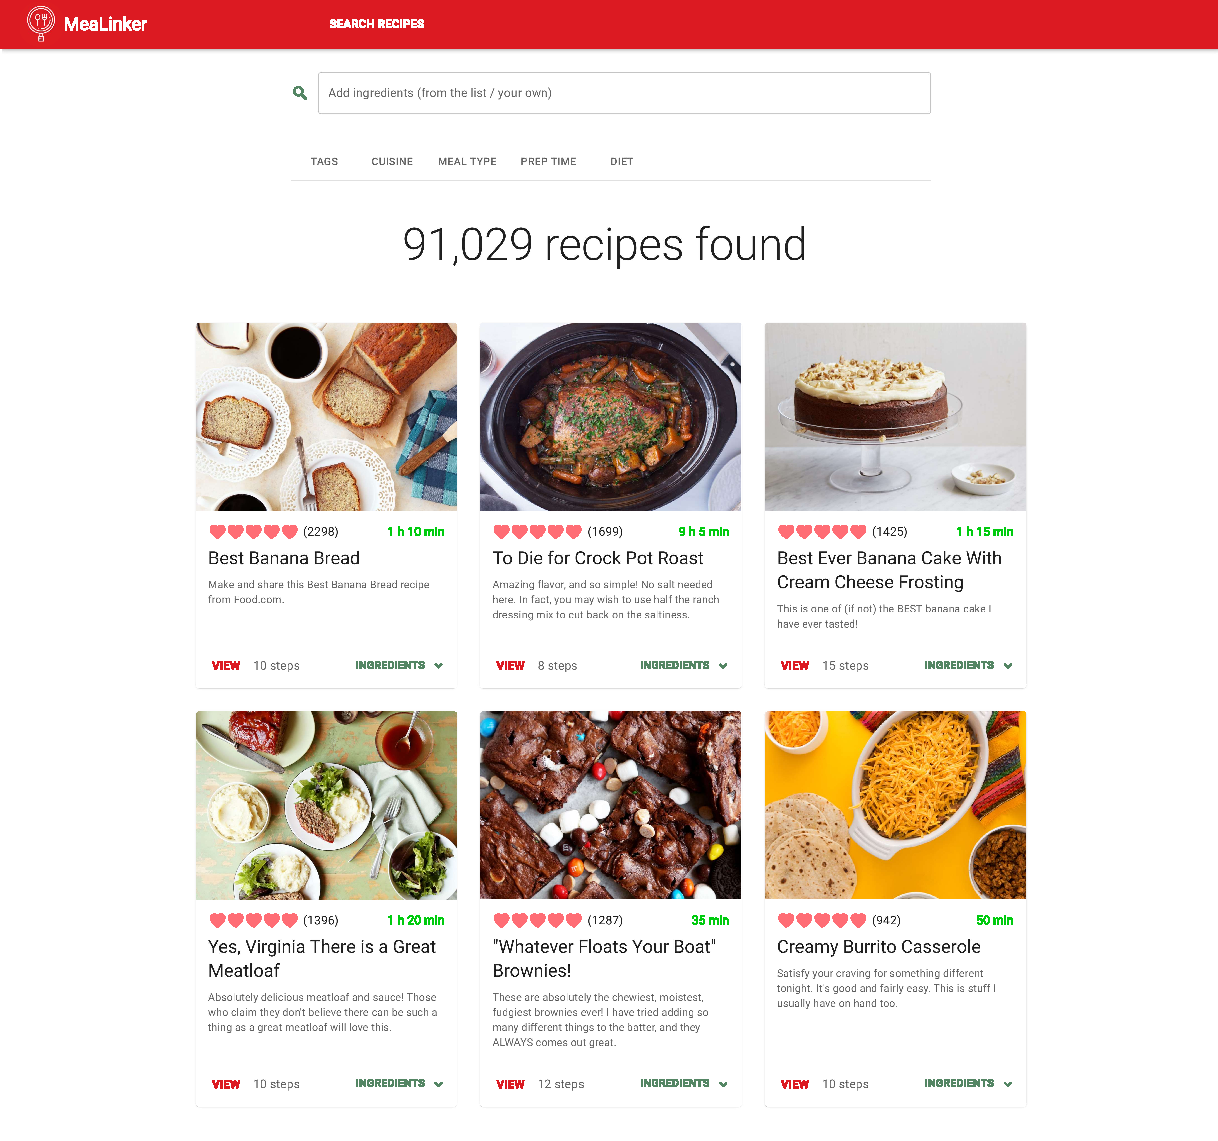
\includegraphics[width=140mm]{../img/homepage}
\caption{Domovská stránka aplikace s vyhledáváním bez zadaných filtrů.}
\label{obr05:homepage}
\end{figure}

\begin{figure}[h!]\centering
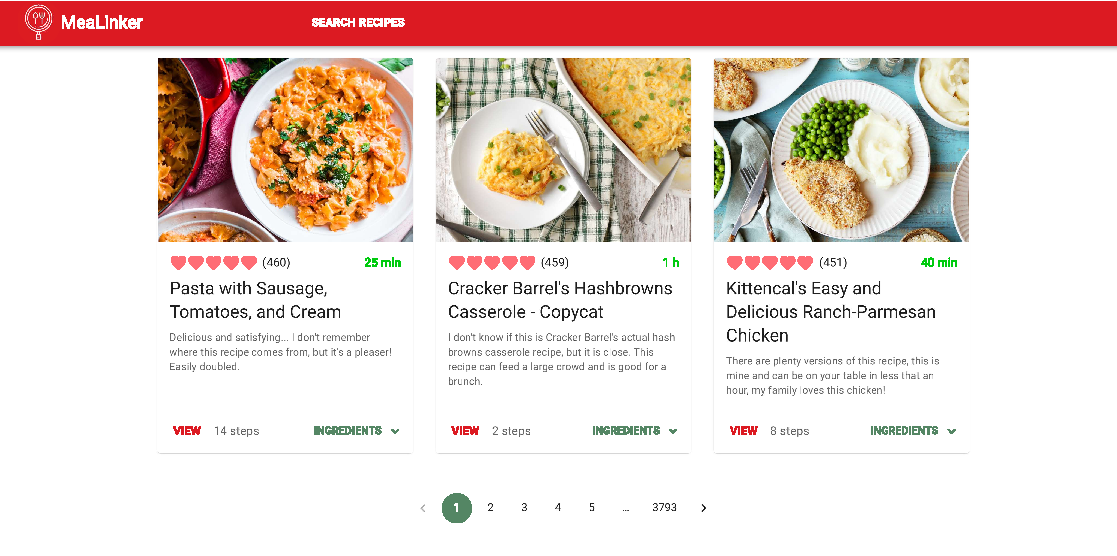
\includegraphics[width=140mm]{../img/pagination}
\caption{Stránkování zpřístupňující všechny nalezené recepty.}
\label{obr05:pagination}
\end{figure}

Aplikace umožňuje vyhledávání receptů upřesnit na základě různých kritérií. Největší důraz je kladen na vyhledávání podle ingrediencí, v~nabídce je ale také filtrování pomocí klíčových slov, kuchyně, typu pokrmu, času přípravy a~diety. Filtry lze libovolně kombinovat a~pro lepší orientaci je u~každé hodnoty napsán počet receptů, které se po přidání tohoto filtru zobrazí. Tomuto stylu vyhledávání se říká fasetová navigace.

Filtry se vždy zobrazují na dvou místech --- v~původním formuláři, do kterého byly vyplněny, ale také pod nadpisem s~počtem vyhledaných receptů. Zde jsou shromážděné filtry ze všech kategorií a~pomocí tlačítka s~ikonou koše je lze snadno odstranit všechny najednou, viz obrázek \ref{obr05:filter-search}. Filtry lze odstranit na libovolném z~těchto míst a~změna se okamžitě projeví i~na místě druhém. Každá změna filtru, ať už přidání nového nebo odebrání stávajícího, spustí automatické vyhledávání receptů. U~filtrů kuchyně a~času přípravy nelze zadat více hodnot najednou.

\begin{figure}[h!]\centering
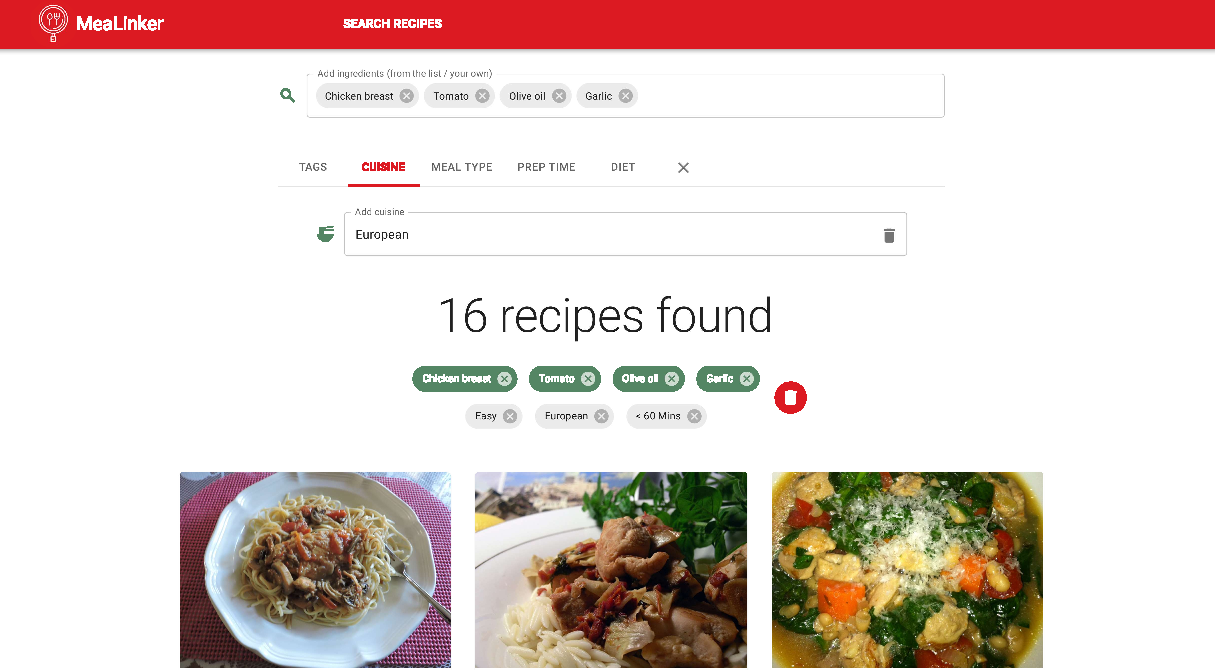
\includegraphics[width=140mm]{../img/filter-search}
\caption{Vyhledávání dle surovin, kuchyně, času přípravy a složitosti.}
\label{obr05:filter-search}
\end{figure}

Pro snadnější orientaci v~nalezených výsledcích lze u~každého receptu rozbalit seznam ingrediencí. V~tomto seznamu jsou zvýrazněny aktuálně vyhledávané ingredience, viz obrázek \ref{obr05:expanded-ingrs}. Seznam je zobrazován přes kartu receptu o~řádek níže a~jeho zavření je potřeba vyřešit ručně kliknutím na ikonu šipky, případně pokračovat na další stranu výsledků.

\begin{figure}[h!]\centering
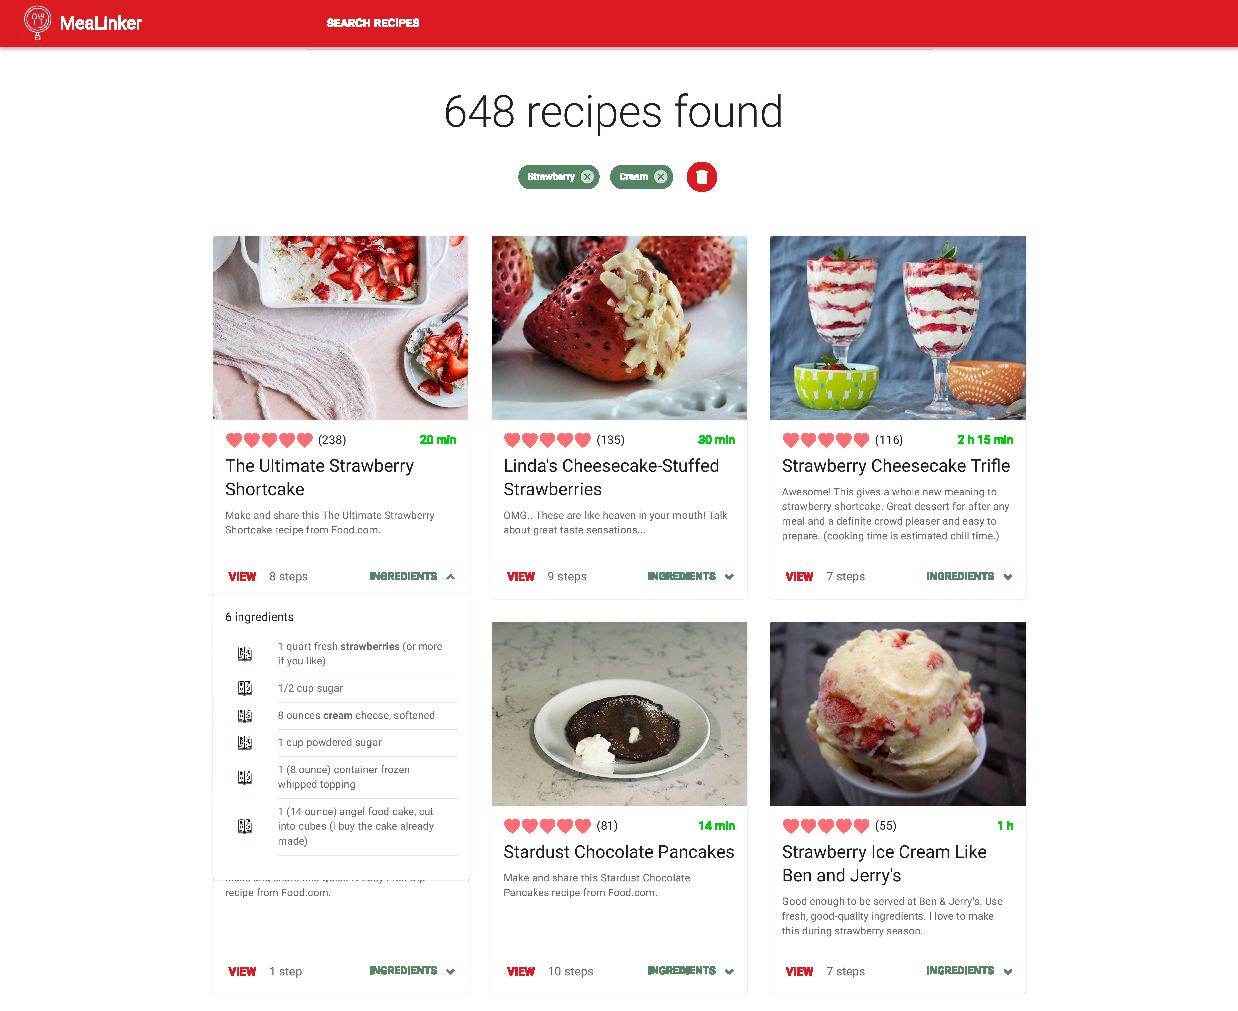
\includegraphics[width=140mm]{../img/expanded-ingrs}
\caption{Rozbalený seznam ingrediencí receptu.}
\label{obr05:expanded-ingrs}
\end{figure}

\section{Detail receptu}

Na obrazovce s~detailem receptu lze vyčíst všechny potřebné informace pro přípravu receptu včetně ingrediencí a~postupu přípravy, viz obrázek \ref{obr05:recipe-detail}. Také je zde k~dispozici tabulka s~nutričními hodnotami. Vybrané ingredience jsou barevně zvýrazněny, což naznačuje, že jsou u~nich k~dispozici rozšiřující informace. Na tyto ingredience lze kliknout, čímž se otevře stránka s~detailem ingredience.

Obrázek receptu je možné přibližovat a~oddalovat pomocí příslušných tlačítek v~levém horním rohu nad fotografií, ale také pomocí touchpadu nebo přidržením klávesy \texttt{Ctrl} a~kolečka myši. Rychlé přiblížení funguje i~přes dvojklik myši. V~pravém horním rohu nad obrázkem je vždy odkaz na zdrojovou stránku receptu, kde jsou typicky doplňující informace v~podobě recenzí nebo podobných receptů. Aktuální verze aplikace neposkytuje modul recenzí, pro jejich prohlížení nebo přidávání je tedy potřeba navštívit zdrojovou stránku.

\begin{figure}[h!]\centering
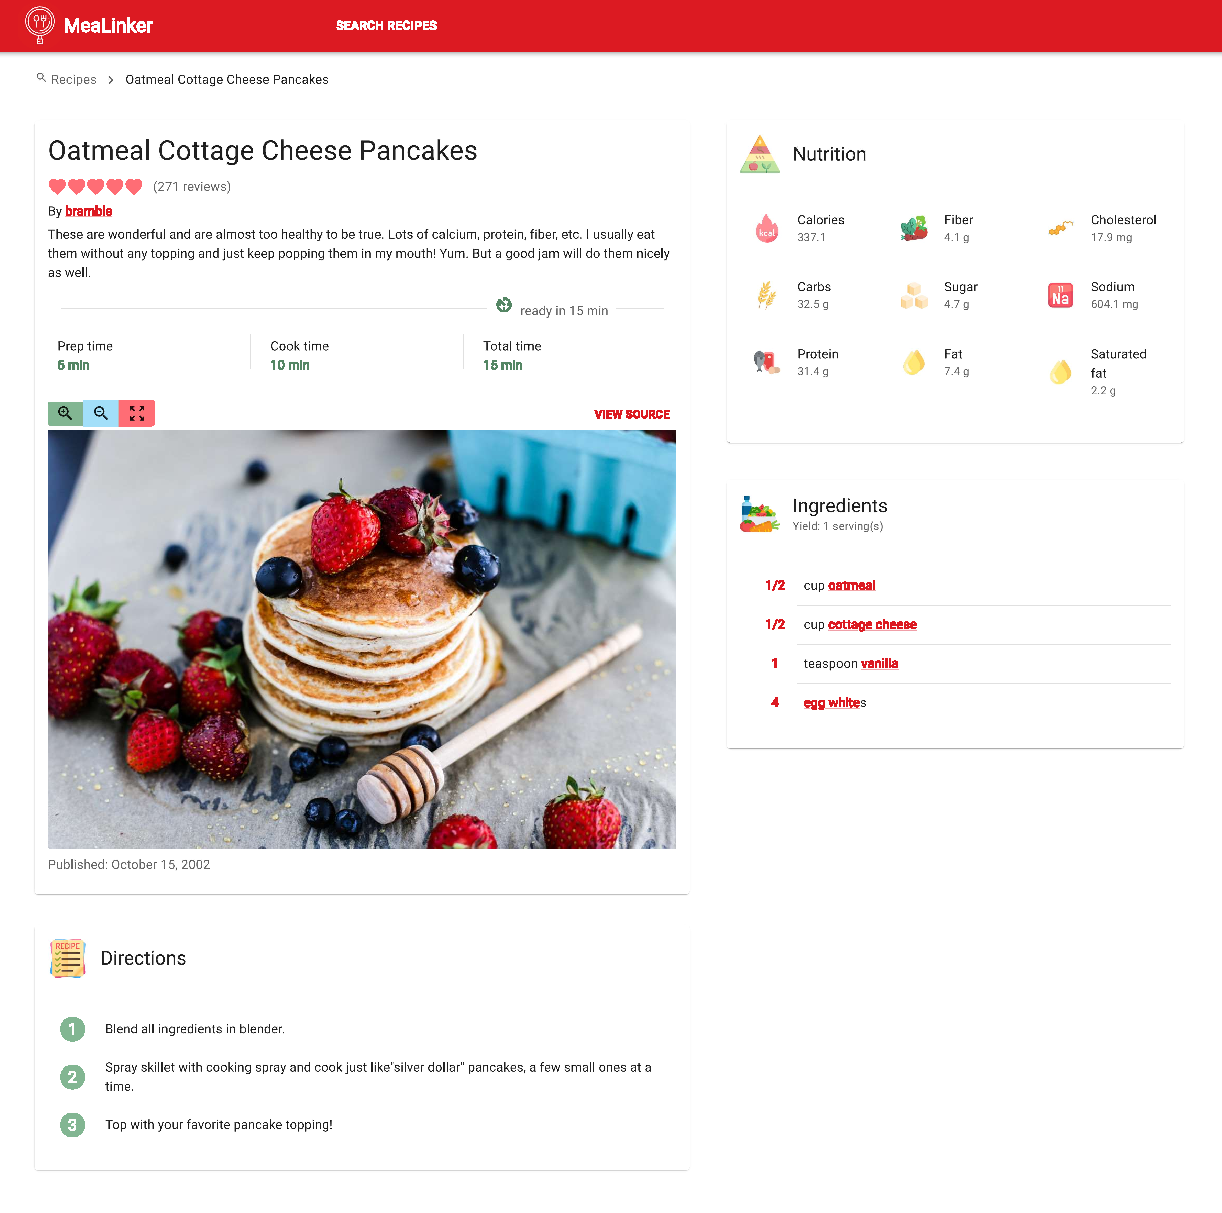
\includegraphics[width=140mm]{../img/recipe-detail}
\caption{Obrazovka detailu receptu.}
\label{obr05:recipe-detail}
\end{figure}

\section{Detail ingredience}

Obsah a~design obrazovky ingredience je proměnlivý podle množství informací, které se k~dané surovině podařilo získat. Standardně obsahuje název, obrázek, popis a~odkaz na zdroj (typicky Wikipedie). Dále volitelně nutriční hodnoty a~kategorie, obojí lze nahlédnout z~obrázku \ref{obr05:ingredient-detail}. Kategorie se dělí na $2$ typy:
\begin{itemize}
    \item Statické kategorie, které mají pouze informativní charakter a~nelze s nimi nijak interagovat, neboť obsahují jen aktuální ingredienci. Jsou označeny světle šedou barvou --- příkladem jsou kategorie \texttt{Persea} nebo \texttt{Trees of Guatemala} na obrázku \ref{obr05:ingredient-detail}.
    \item Rozbalovací kategorie, které obsahují aspoň $1$~ingredienci odlišnou od aktuální ingredience. Přísady uložené v~těchto kategoriích mají výraznější zelenou barvu (viz obrázek \ref{obr05:ingredient-categories}) a~kliknutím je lze otevřít.
\end{itemize}

\begin{figure}[p]\centering
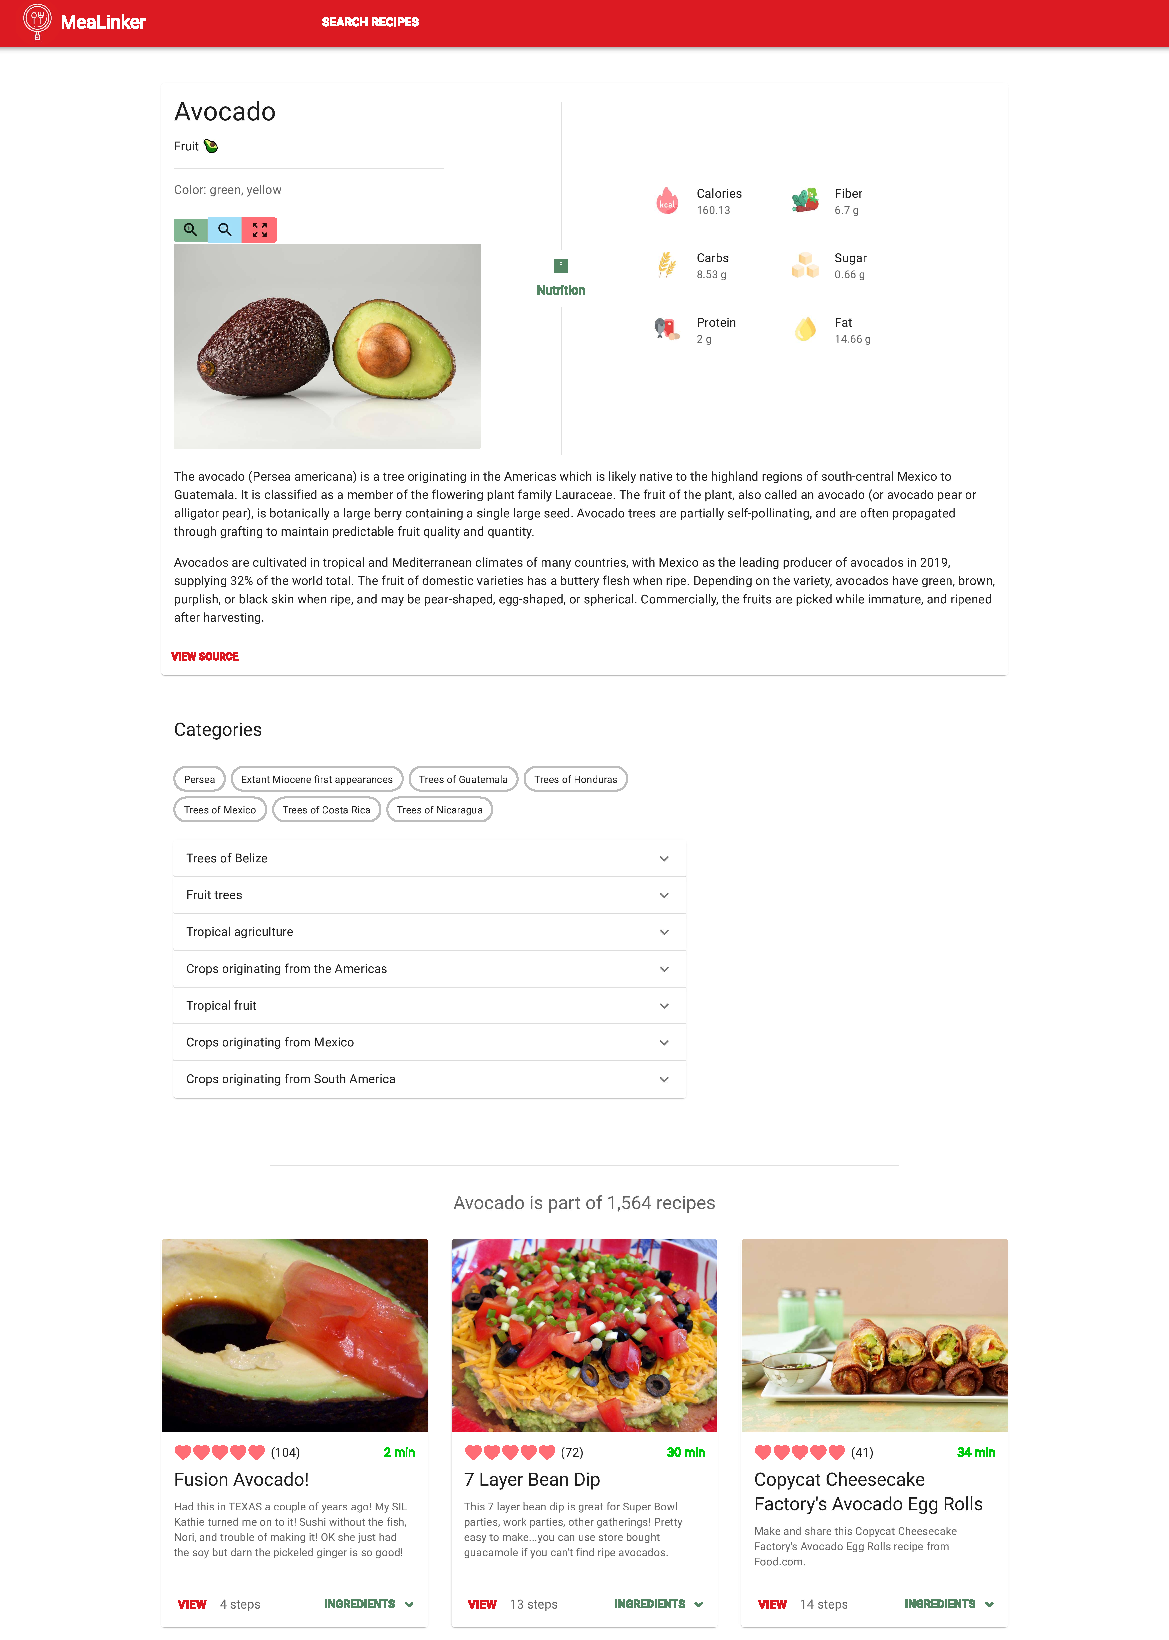
\includegraphics[width=140mm]{../img/ingredient-detail}
\caption{Obrazovka ingredience s~nutričními hodnotami a~kategoriemi.}
\label{obr05:ingredient-detail}
\end{figure}

Pokud se jedná o~takzvaně složenou ingredienci, tak lze na stránce najít přísady, ze kterých je tato ingredience vyrobená. Tato informace je prezentována ve vnořené kartě s~názvem \texttt{Made\,of}. Příkladem je ingredience \texttt{Guacamole} (obrázek \ref{obr05:ingredient-categories}), kterou je možné vyrobit ze základních ingrediencí avokáda, cibule, limetky, soli a~koriandru. U~některých surovin je pod názvem uvedeno místo původu, jak je možné vidět opět na obrázku \ref{obr05:ingredient-categories}. Z~doplňujících informací lze u~některých surovin nalézt barvu a~unicode znak (například u~avokáda z~obrázku \ref{obr05:ingredient-detail}).

Pod informacemi k~ingredienci následují karty receptů obsahující aktuální ingredienci. Rozložení karet je identické s~vyhledávací obrazovkou receptů a~rovněž je zde možné prohlížet více stran výsledků. 

\begin{figure}[h!]\centering
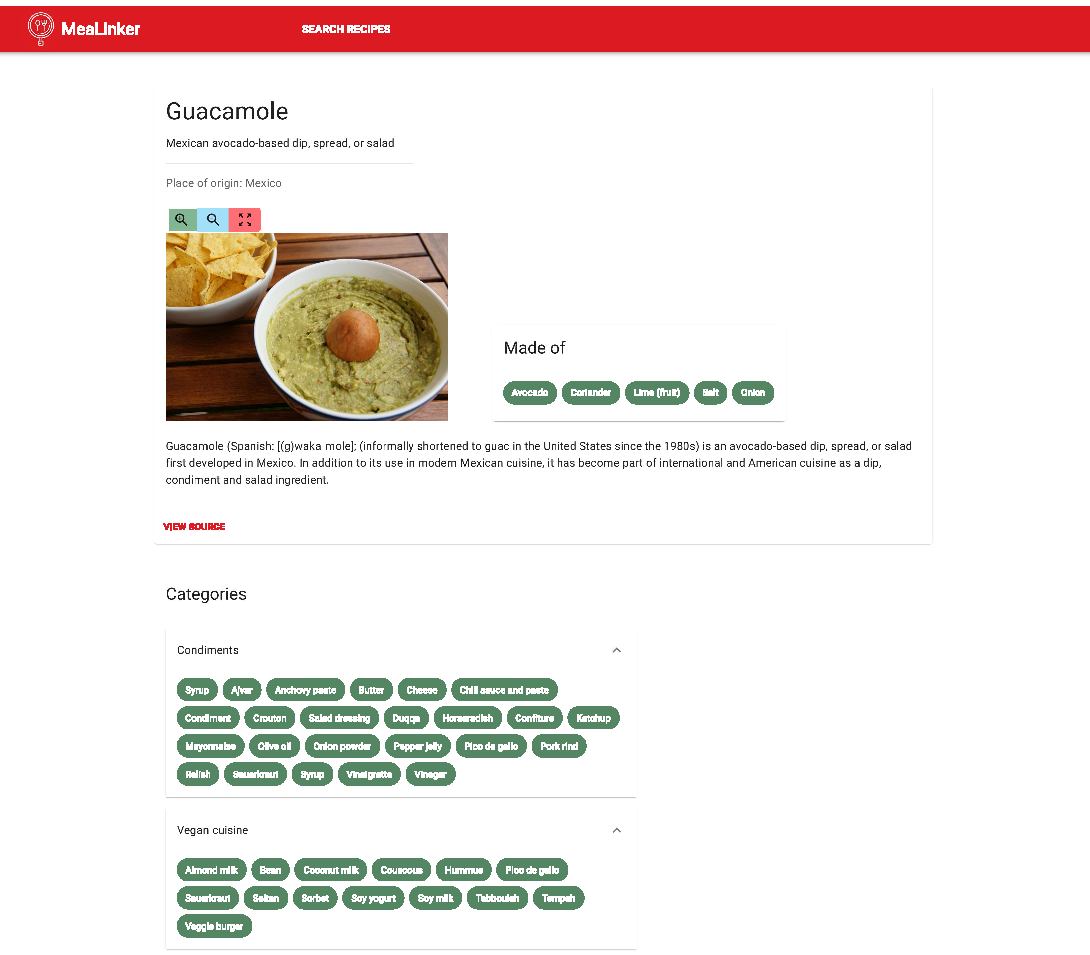
\includegraphics[width=140mm]{../img/ingredient-categories}
\caption{Obrazovka detailu ingredience s rozbalenými kategoriemi.}
\label{obr05:ingredient-categories}
\end{figure}

\chapter*{Závěr}
\addcontentsline{toc}{chapter}{Závěr}

Cílem této bakalářské práce bylo vytvořit aplikaci pro vyhledávání receptů, která agreguje data z~různých zdrojů s~využitím principu propojených dat. Demonstrovali jsme přínosy a~úskalí statických datasetů i~vlastní extrakce dat. Dále jsme zapojili informace z~otevřených znalostních grafů, které nám umožnily nejen rozšířit data o~jednotlivých ingrediencích, ale také objevit nová spojení mezi přísadami a~tranzitivně i~recepty.

V~prvotní fázi vývoje byly zadefinovány funkční i~nefunkční požadavky aplikace, na základě kterých byla navržena architektura a~uživatelské rozhraní. Výběr požadavků byl veden analýzou existujících webových aplikací pro vyhledávání receptů. Naše práce si totiž stanovila cíl propojit užitečné funkce z~osvědčených aplikací a~nabídnout přidanou hodnotu díky jejich zkombinování v~rámci jedné aplikace. Volba klíčových technologií se ukázala jako vhodná pro naplnění požadavků.

Práce se soustředila pouze na získání a~prezentaci existujících dat receptů a~ingrediencí. Přidávání nových dokumentů prostřednictvím uživatelského rozhraní aplikace bude otázkou dalšího vývoje spolu s~registrací uživatelů, ukládání oblíbených receptů, nákupního seznamu a~dalších souvisejících funkcí.

Zkorigování dat z~více zdrojů vyžaduje poměrně velké množství manuální práce, neboť mohou obsahovat řadu odchylek od standardního formátu. Pokud bychom ale měli k~dispozici dostatečnou časovou dotaci a~výpočetní prostředky, aplikace by mohla vyniknout právě velkým množstvím dostupných dat. S~rostoucí datovou sadou bychom byli schopni nabídnout rozmanitější filtrování výsledků nebo také personalizované návrhy receptů.

Aktuální řešení je připraveno pro nasazení a~vývoj dalších funkcionalit. Postup extrakce a~ukládání nových dokumentů je v~co největší míře automatizován pomocí vlastních skriptů, stejně jako definice schématu pro vyhledávání na základě indexů.

%%% Seznam použité literatury
%%% Seznam použité literatury (bibliografie)
%%%
%%% Pro vytváření bibliografie používáme bibTeX. Ten zpracovává
%%% citace v textu (např. makro \cite{...}) a vyhledává k nim literaturu
%%% v souboru literatura.bib.
%%%
%%% Příkaz \bibliographystyle určuje, jakým stylem budou citovány odkazy
%%% v textu. V závorce je název zvoleného souboru .bst. Styly plainnat
%%% a unsrt jsou standardní součástí latexových distribucí. Styl czplainnat
%%% je dodáván s touto šablonou a bibTeX ho hledá v aktuálním adresáři.

\bibliographystyle{czplainnat}    %% Autor (rok) s českými spojkami
% \bibliographystyle{plainnat}    %% Autor (rok) s anglickými spojkami
% \bibliographystyle{unsrt}       %% [číslo]

\renewcommand{\bibname}{Seznam použité literatury}

%%% Vytvoření seznamu literatury. Pozor, pokud jste necitovali ani jednu
%%% položku, seznam se automaticky vynechá.

\bibliography{literatura}

%%% Kdybyste chtěli bibliografii vytvářet ručně (bez bibTeXu), lze to udělat
%%% následovně. V takovém případě se řiďte normou ISO 690 a zvyklostmi v oboru.

% \begin{thebibliography}{99}
%
% \bibitem{lamport94}
%   {\sc Lamport,} Leslie.
%   \emph{\LaTeX: A Document Preparation System}.
%   2. vydání.
%   Massachusetts: Addison Wesley, 1994.
%   ISBN 0-201-52983-1.
%
% \end{thebibliography}


%%% Obrázky v bakalářské práci
%%% (pokud jich je malé množství, obvykle není třeba seznam uvádět)
\listoffigures

%%% Tabulky v bakalářské práci (opět nemusí být nutné uvádět)
%%% U matematických prací může být lepší přemístit seznam tabulek na začátek práce.
% \listoftables

%%% Přílohy k bakalářské práci, existují-li. Každá příloha musí být alespoň jednou
%%% odkazována z vlastního textu práce. Přílohy se číslují.
%%%
%%% Do tištěné verze se spíše hodí přílohy, které lze číst a prohlížet (dodatečné
%%% tabulky a grafy, různé textové doplňky, ukázky výstupů z počítačových programů,
%%% apod.). Do elektronické verze se hodí přílohy, které budou spíše používány
%%% v elektronické podobě než čteny (zdrojové kódy programů, datové soubory,
%%% interaktivní grafy apod.). Elektronické přílohy se nahrávají do SISu a lze
%%% je také do práce vložit na CD/DVD. Povolené formáty souborů specifikuje
%%% opatření rektora č. 72/2017.
\appendix
\chapter{Přílohy}

\section{Instalace a spuštění aplikace}

Konfiguraci aplikace rozdělíme do $3$ fází:

\begin{enumerate}
    \item Příprava dat
    \item Persistence dat
    \item Spuštění aplikace
\end{enumerate}

Předpokládá se nainstalovaný runtime Node.js pro vývoj v~jazyce JavaScript s výchozím správcem balíčků npm. Systémy Apache Solr a~Silk Workbench byly zprovozněny pomocí Dockeru jako samostatné kontejnery, je ale možné zvolit jiný způsob instalace. Ke zpracování dat receptů a~ingrediencí jsou přiloženy shellové skripty pro systémy Windows i~Linux. Počínaje konfiguračními skripty \texttt{build.bat}, respektive \texttt{build.sh}, z~adresáře \texttt{data} se rekurzivně volají skripty z~vnořených adresářů. Dále jsou připraveny skripty \texttt{run.bat} a~\texttt{run.sh} pro spuštění extrakce, konverze a~následného nahrání dokumentů do databáze. Jednotlivé JavaScriptové programy lze spouštět samostatně příkazem \texttt{node\,script.js}. Často budeme potřebovat spustit jen některé fáze, zejména extrakce bude vzhledem k~objemu dat výjimečnou záležitostí. Shellové skripty tak často poslouží spíše jako dokumentace správného pořadí jednotlivých skriptů. Konstanty potřebné pro konfiguraci jsou obvykle soustředěny v~souborech \texttt{constants.js} a~\texttt{config.js}. Jejich hodnoty lze přizpůsobit dle potřeby, například omezit počet receptů, které se mají extrahovat z~webové aplikace pomocí Apify actora.

\subsection{Příprava dat}

Předpokládáme následující nainstalované nástroje:

\begin{itemize}
    \item Python
    \item Apify CLI\footnote{https://www.npmjs.com/package/apify-cli/v/0.1.2}
    \item Silk Workbench\footnote{https://hub.docker.com/r/silkframework/silk-workbench}
\end{itemize}

V~rámci fáze extrakce a~předzpracování dat je potřeba stáhnout datovou sadu \emph{Food.com Recipes and~Interactions}\footnote{https://www.kaggle.com/datasets/shuyangli94/food-com-recipes-and-user-interactions} z~Kaggle. Soubory \texttt{RAW\underline{{ }}recipes.csv} a~\texttt{PP\underline{{ }}recipes.csv} patří do adresáře \texttt{data/resources/foodcom/recipes}. Dále je potřeba umístit \texttt{ingr\underline{{ }}map.csv} do \texttt{data/resources/foodcom/ingredients}. Následně jsou připraveny skripty pro konverzi a~extrakci dat z~webových aplikací Food.com a~Allrecipes. Pro spuštění \texttt{run-venv.bat}, eventuálně \texttt{run-venv.sh} uvnitř adresáře \texttt{data/resources/foodcom/ingredients} je potřeba mít aktivováno virtuální prostředí pro vývoj v~jazyce Python s~nainstalovanou knihovnou pickle.

Ve všech adresářích obsahujících soubor \texttt{package.json} je potřeba použít příkaz \texttt{npm\,install}. Inicializace Apify actorů v~adresářích \texttt{food-com-scraper} a~\texttt{allrecipes-scraper} se provede standardními příkazy \texttt{npm\,install} a~dále \texttt{apify\,init}, který vytvoří potřebné podadresáře včetně \texttt{apify\underline{{ }}storage}. Zejména adresáře s~actory jsou zcela nezávislé na kontextu zbytku aplikace, aby bylo co nejsnadnější je v případě potřeby migrovat na cloudovou platformu Apify, pro kterou jsou primárně určeny.

Dále je potřeba zkopírovat vygenerované datasety ingrediencí v RDF formátu Turtle z~adresářů \texttt{ingredients} do aplikace Silk Workbench a~vytvořit pro ně úlohy linkování s~otevřenými znalostními grafy DBpedia a~Wikidata. V~podadresářích \texttt{rdf-data} uvnitř adresářů \texttt{foodcom} a~\texttt{allrecipes} je uložen konfigurační XML soubor vygenerovaný ze Silk Workbench. Pomocí něj je možné úlohu spustit z~příkazové řádky, naše řešení ale tohoto přístupu nevyužívá. Datasety s~propojenými entitami jsou očekávány v~adresářích \texttt{rdf-data} ve formátu N-triples.

\subsection{Persistence dat}

Předpokládáme nainstalovanou instanci systému Apache CouchDB s~platnými přihlašovacími údaji a~přístupem do administrace skrze webovou aplikaci \-Fauxton. Dále instalaci platformy Apache Solr s~vytvořeným jádrem \texttt{recipes}.

Extrahovaná a~vyčištěná data jsou ukládána do databáze CouchDB. Příslušné skripty a~konfigurační soubory najdeme v~adresáři \texttt{data/database} a~jsou volány pomocí automatizovaného skriptu \texttt{run} z~kořenového adresáře \texttt{data}. Heslo pro přihlášení do databáze je potřeba uložit jako proměnnou prostředí pod názvem \texttt{COUCHDB\underline{{ }}PASSWORD} nebo změnit nastavení v souboru \texttt{config.js}.

Následuje vytvoření indexů a~odpovídajících dokumentů receptů pro platformu Solr. Související skripty jsou v~adresáři \texttt{data/solr}. Dokumenty receptů jsou extrahovány přímo z~databáze CouchDB, což by mělo usnadnit situaci, kdy by instance CouchDB a~Solr běžely na různých zařízeních.

\subsection{Spuštění aplikace}

Kód aplikace je soustředěn v~adresáři \texttt{app}, který je dále rozdělen na \texttt{frontend} a~\texttt{backend}. K~inicializace obou částí aplikace stačí nainstalovat závislosti dle \texttt{package.json} pomocí \texttt{npm\,install}. Pro následné spuštění serverové části aplikace je potřeba spustit z~umístění \texttt{backend} příkazy \texttt{npm\,run\,build} pro automatickou transpilaci z~TypeScriptu do JavaScriptu a~\texttt{npm\,start} k~samotnému spuštění aplikace. Pro úspěšný start musí být k~dispozici CouchDB i~Solr na adresách specifikovaných v~příslušných souborech \texttt{config.js}. Single-page aplikaci lze spustit ve vývojářském módu pomocí \texttt{npm\,start} z~adresáře \texttt{frontend}. Veškeré změny v~kódu backendu i~frontendu se po uložení automaticky projeví v~aplikaci běžící ve webovém prohlížeči. Produkční verze aplikace je do adresáře \texttt{frontend/build} generována příkazem \texttt{npm\,run\,build}. Následně lze spustit pomocí \texttt{serve\,-s\,build}.

\pagebreak
\section{Hledání linků mezi datasety ingrediencí}

\begin{figure}[h!]\centering
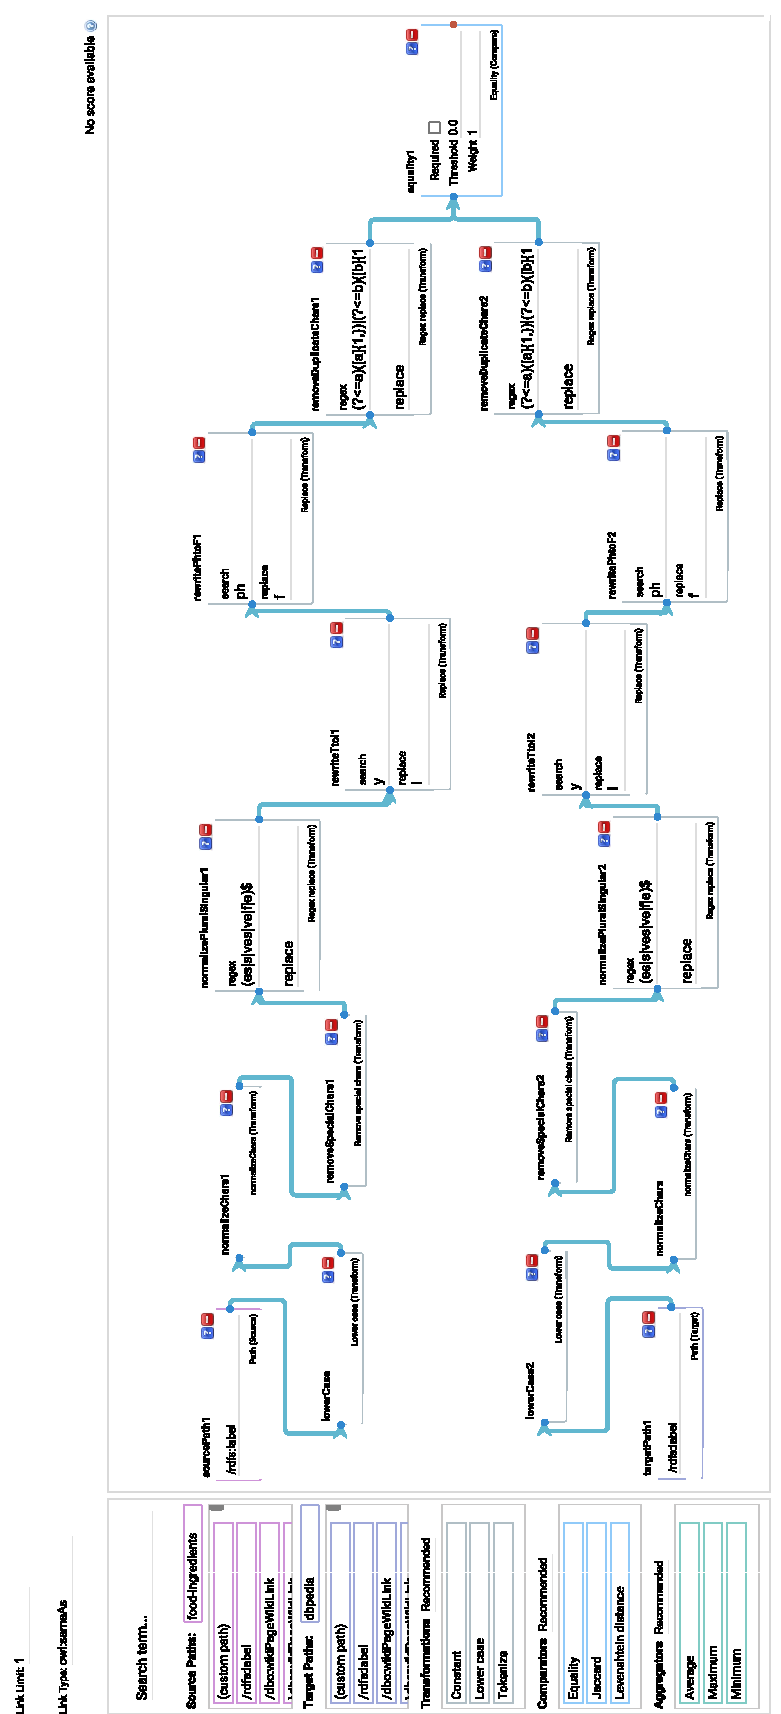
\includegraphics[height=220mm]{../img/silk-workbench}
\caption{Grafické znázornění úlohy linkování v aplikaci Silk Workbench.}
\label{obr0a:silk-workbench}
\end{figure}

\section{Výsledky testování SUS}

Pro otestování UX designu naší aplikace jsme využili nástroj System Usability Scale neboli SUS \citep{sus-test}. Testující dostali $5$ jednoduchých úkolů uvedených v kapitole o testování a vyzkoušeli si skrze ně běžnou práci s aplikací. Posledním úkolem bylo zodpovědět $10$ standardizovaných otázek dle SUS dotazníku na škále od $1$ do $5$, kde $1$ představuje \uv{silně nesouhlasím} a $5$ naopak \uv{silně souhlasím}. 

\subsection{Formát dotazníku}
Otázky jsme dle vzoru z anglického zdroje zformulovali následovně \citep{sus-adobe}:

\begin{enumerate}
    \item Myslím, že bych rád aplikaci využíval pravidelně.
    \item Aplikace mi připadá zbytečně složitá.
    \item S aplikací se mi pracovalo snadno.
    \item Myslím, že bych potřeboval technickou podporu.
    \item Myslím, že funkce byly v aplikaci dobře integrovány.
    \item Zdá se mi, že aplikace byla příliš nekonzistentní.
    \item Domnívám se, že většina lidí by se naučila aplikaci používat velmi rychle.
    \item Ovládání aplikace mi připadalo dost těžkopádné.
    \item Při používání aplikace jsem se cítil velmi jistý.
    \item Musel jsem se naučit hodně věcí, než jsem mohl začít aplikaci používat.
\end{enumerate}

\subsection{Postup výpočtu skóre}

Algoritmus výpočtu skóre je následující \citep{sus-adobe}:

\begin{enumerate}
    \item Zvol proměnnou $X$ jako součet celkového skóre otázek s lichým pořadím snížený o hodnotu $5$.
    \item Zvol proměnnou $Y$ jako výsledek celkového skóre otázek se sudým pořadím odečtený od $25$.
    \item Sečti hodnoty proměnných $X$, $Y$ a výsledek vynásob koeficientem $2,5$.
\end{enumerate}

Odpověď na i-tou otázku označme $a_i$.

$X := \sum a_i$ pro $i \in \{1,3,5,7,9\}$

$Y := \sum a_j$ pro $j \in \{2,4,6,8,10\}$

$Z := ( \,X + Y\,)\,\cdot\,2,5$

\subsection{Výpočet skóre}

Odpovědi vyjádříme pomocí uspořádaných $10$-tic s~prvky v~pořadí od $1$.~do $10$. odpovědi a~s~indexem odpovídajícím pořadí respondenta. Celkem dotazník zodpověděli $4$ respondenti.

\subsubsection{První respondent}

$v_1 := (\,4,1,4,1,5,2,5,1,5,1\,)$

$X_1 := (\,4 + 4 + 5 + 5 + 5\,) - 5 = 18\,$

$Y_1 := 25 - (\,1 + 1 + 2 + 1 + 1\,) = 19\,$

$Z_1 := ( \,18 + 19\,)\,\cdot\,2,5 = 92,5$

\subsubsection{Druhý respondent}

$v_2 := (\,4,2,5,1,4,1,5,1,5,1\,)$

$X_2 := (\,4 + 5 + 4 + 5 + 5\,) - 5 = 18\,$

$Y_2 := 25 - (\,2 + 1 + 1 + 1 + 1\,) = 19\,$

$Z_2 := ( \,18 + 19\,)\,\cdot\,2,5 = 92,5$

\subsubsection{Třetí respondent}

$v_3 := (\,5,2,5,1,5,1,5,1,4,1\,)$

$X_3 := (\,5 + 5 + 5 + 5 + 4\,) - 5 = 19\,$

$Y_3 := 25 - (\,2 + 1 + 1 + 1 + 1\,) = 19\,$

$Z_3 := ( \,19 + 19\,)\,\cdot\,2,5 = 95$

\subsubsection{Čtvrtý respondent}

$v_4 := (\,4,2,4,1,5,1,5,1,5,1\,)$

$X_4 := (\,4 + 4 + 5 + 5 + 5\,) - 5 = 18\,$

$Y_4 := 25 - (\,2 + 1 + 1 + 1 + 1\,) = 19\,$

$Z_4 := ( \,18 + 19\,)\,\cdot\,2,5 = 92,5$

\subsubsection{Průměrné skóre}

Finální hodnocení $R$ vypočteme jako průměr výsledků jednotlivých respondentů:

$R := \frac{Z_1 + Z_2 + Z_3 + Z_4}{4} = \frac{(\,92,5\,\cdot\,3\,)\,+\,95}{4} = 93,125$

\openright
\end{document}
